\documentclass{book}
\usepackage[a4paper,top=2.5cm,bottom=2.5cm,left=2.5cm,right=2.5cm]{geometry}
\usepackage{makeidx}
\usepackage{natbib}
\usepackage{graphicx}
\usepackage{multicol}
\usepackage{float}
\usepackage{listings}
\usepackage{color}
\usepackage{ifthen}
\usepackage[table]{xcolor}
\usepackage{textcomp}
\usepackage{alltt}
\usepackage{ifpdf}
\ifpdf
\usepackage[pdftex,
            pagebackref=true,
            colorlinks=true,
            linkcolor=blue,
            unicode
           ]{hyperref}
\else
\usepackage[ps2pdf,
            pagebackref=true,
            colorlinks=true,
            linkcolor=blue,
            unicode
           ]{hyperref}
\usepackage{pspicture}
\fi
\usepackage[utf8]{inputenc}
\usepackage{mathptmx}
\usepackage[scaled=.90]{helvet}
\usepackage{courier}
\usepackage{sectsty}
\usepackage{amssymb}
\usepackage[titles]{tocloft}
\usepackage{doxygen}
\lstset{language=C++,inputencoding=utf8,basicstyle=\footnotesize,breaklines=true,breakatwhitespace=true,tabsize=4,numbers=left }
\makeindex
\setcounter{tocdepth}{3}
\renewcommand{\footrulewidth}{0.4pt}
\renewcommand{\familydefault}{\sfdefault}
\hfuzz=15pt
\setlength{\emergencystretch}{15pt}
\hbadness=750
\tolerance=750
\begin{document}
\hypersetup{pageanchor=false,citecolor=blue}
\begin{titlepage}
\vspace*{7cm}
\begin{center}
{\Large A\-L\-R \\[1ex]\large v1.\-0 }\\
\vspace*{1cm}
{\large Generated by Doxygen 1.8.1.2}\\
\vspace*{0.5cm}
{\small Thu Dec 18 2014 02:50:23}\\
\end{center}
\end{titlepage}
\clearemptydoublepage
\pagenumbering{roman}
\tableofcontents
\clearemptydoublepage
\pagenumbering{arabic}
\hypersetup{pageanchor=true,citecolor=blue}
\chapter{Data Structure Index}
\section{Data Structures}
Here are the data structures with brief descriptions\-:\begin{DoxyCompactList}
\item\contentsline{section}{\hyperlink{structautomata__t}{automata\-\_\-t} \\*Structure that represents dynamically generated automata feat\-: Feature structure mtx\-: Matrix structure stat\-: Statistic structure range\-: Range structure state\-: Current state splits\-: Number of splits on \mbox{[}0, 1\mbox{]} sym\-\_\-class\-\_\-num\-: Number of symbol classes max\-\_\-los\-: Max feature value of generated data min\-\_\-los\-: Min feature value of generated data min\-\_\-tab\-: Min feature values of read data max\-\_\-tab\-: Max feature values of read data is\-\_\-read\-: Is data read from files? fuzzy\-: Is automata fuzzy? }{\pageref{structautomata__t}}{}
\item\contentsline{section}{\hyperlink{structfeature__t}{feature\-\_\-t} \\*Structure that represents feature vector feat\-: Feature values vector size\-: Vector size correct\-: Correct state determin\-\_\-splits\-: Vector of deterministic splits A\-\_\-1, A\-\_\-3 .... A\-\_\-6, A\-\_\-2 }{\pageref{structfeature__t}}{}
\item\contentsline{section}{\hyperlink{structmatrix__t}{matrix\-\_\-t} \\*3d matrix structure m \-:= split n, k \-:= states add \-:= add operator handler mul \-:= mul operator handler }{\pageref{structmatrix__t}}{}
\item\contentsline{section}{\hyperlink{structParticle}{Particle} }{\pageref{structParticle}}{}
\item\contentsline{section}{\hyperlink{structpso__params__t}{pso\-\_\-params\-\_\-t} \\*P\-S\-O parameters iterations\-: Number of P\-S\-O iterations swarmsize\-: Swarm size trace\-: Print trace? fnscale\-: Error scale w\-: The exploitation constant cp\-: Local exploration constant cg\-: Global exploration constant }{\pageref{structpso__params__t}}{}
\item\contentsline{section}{\hyperlink{structstatistic__t}{statistic\-\_\-t} \\*Structure that represents statistics of correctly distinguished symbols whole\-: Whole number of input features errors\-: Number of errors during the automata work fuzzy\-\_\-errors\-: Number of errors during the fuzzy automata work }{\pageref{structstatistic__t}}{}
\end{DoxyCompactList}

\chapter{File Index}
\section{File List}
Here is a list of all files with brief descriptions\-:\begin{DoxyCompactList}
\item\contentsline{section}{\hyperlink{alr_8c}{alr.\-c} }{\pageref{alr_8c}}{}
\item\contentsline{section}{\hyperlink{alr_8h}{alr.\-h} }{\pageref{alr_8h}}{}
\item\contentsline{section}{\hyperlink{main_8c}{main.\-c} }{\pageref{main_8c}}{}
\item\contentsline{section}{\hyperlink{matrix_8c}{matrix.\-c} }{\pageref{matrix_8c}}{}
\item\contentsline{section}{\hyperlink{matrix_8h}{matrix.\-h} }{\pageref{matrix_8h}}{}
\item\contentsline{section}{\hyperlink{swarm_8c}{swarm.\-c} }{\pageref{swarm_8c}}{}
\item\contentsline{section}{\hyperlink{swarm_8h}{swarm.\-h} }{\pageref{swarm_8h}}{}
\item\contentsline{section}{\hyperlink{syswrap_8c}{syswrap.\-c} }{\pageref{syswrap_8c}}{}
\item\contentsline{section}{\hyperlink{syswrap_8h}{syswrap.\-h} }{\pageref{syswrap_8h}}{}
\item\contentsline{section}{\hyperlink{types_8h}{types.\-h} }{\pageref{types_8h}}{}
\end{DoxyCompactList}

\chapter{Data Structure Documentation}
\hypertarget{structautomata__t}{\section{automata\-\_\-t Struct Reference}
\label{structautomata__t}\index{automata\-\_\-t@{automata\-\_\-t}}
}


structure that represents dynamically generated automata feat\-: Feature structure mtx\-: Matrix structure stat\-: Statistic structure range\-: Range structure state\-: Current state splits\-: Number of splits on \mbox{[}0, 1\mbox{]} sym\-\_\-class\-\_\-num\-: Number of symbol classes max\-\_\-los\-: Max feature value of generated data min\-\_\-los\-: Min feature value of generated data min\-\_\-tab\-: Min feature values of read data max\-\_\-tab\-: Max feature values of read data is\-\_\-read\-: Is data read from files? fuzzy\-: Is automata fuzzy?  




{\ttfamily \#include $<$alr.\-h$>$}



Collaboration diagram for automata\-\_\-t\-:\nopagebreak
\begin{figure}[H]
\begin{center}
\leavevmode
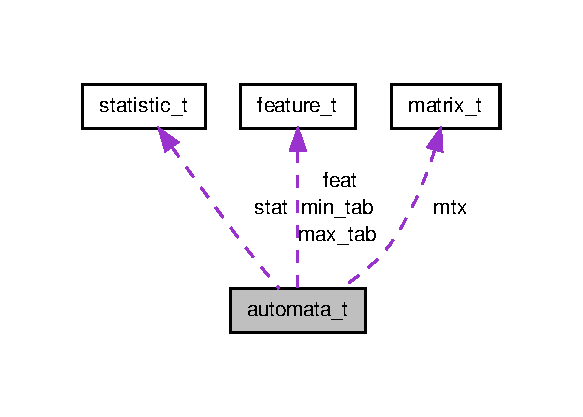
\includegraphics[width=280pt]{structautomata__t__coll__graph}
\end{center}
\end{figure}
\subsection*{Data Fields}
\begin{DoxyCompactItemize}
\item 
\hyperlink{structfeature__t}{feature\-\_\-t} \hyperlink{structautomata__t_aea937bcdfee70c1a1c33ebdd8abe22e4}{feat}
\item 
double \hyperlink{structautomata__t_ac1b32f1fedaa18ce4660e0c861d02499}{max\-\_\-los}
\item 
double \hyperlink{structautomata__t_a1c154215cdc0a2385e5ef4d638b90d7f}{min\-\_\-los}
\item 
\hyperlink{structfeature__t}{feature\-\_\-t} \hyperlink{structautomata__t_a42a70ea18f8540b5b62c425a51a716ca}{min\-\_\-tab}
\item 
\hyperlink{structfeature__t}{feature\-\_\-t} \hyperlink{structautomata__t_a6f76cc86cd6b6a69a21293f071391122}{max\-\_\-tab}
\item 
int \hyperlink{structautomata__t_a2d180cfe5698f6f9999b03cebaf83fcd}{is\-\_\-read}
\item 
\hyperlink{structmatrix__t}{matrix\-\_\-t} \hyperlink{structautomata__t_ad622b3580c94fcb06420e0d67dccfa3d}{mtx}
\item 
\hyperlink{structstatistic__t}{statistic\-\_\-t} \hyperlink{structautomata__t_ab202220b21f1095ec7837e4c14b0e9ed}{stat}
\item 
\hyperlink{types_8h_ac2a93159315d50befc9dd047d7de19a3}{symbol\-\_\-class} \hyperlink{structautomata__t_a967887d248745296590c426dd1046cea}{state}
\item 
\hyperlink{types_8h_a4717ab46b712567c1482ad0f5b910027}{msize\-\_\-t} \hyperlink{structautomata__t_a419b230963c5665dfe3b183ebf656708}{splits}
\item 
\hyperlink{types_8h_a4717ab46b712567c1482ad0f5b910027}{msize\-\_\-t} \hyperlink{structautomata__t_af7d9c374fd308653e15298ed62c36d59}{sym\-\_\-class\-\_\-num}
\item 
\hyperlink{types_8h_a9052d9742e283c5c2169b5b06f8245f0}{feat\-\_\-t} \hyperlink{structautomata__t_afcdd7f850b7d570e79cb82885fd973d1}{range}
\item 
\hyperlink{types_8h_a57c3b7201116536b822f0f8520aa99c7}{bool\-\_\-t} \hyperlink{structautomata__t_aeb015ceca00323d9a3ef30c7cb219246}{fuzzy}
\end{DoxyCompactItemize}


\subsection{Detailed Description}
structure that represents dynamically generated automata feat\-: Feature structure mtx\-: Matrix structure stat\-: Statistic structure range\-: Range structure state\-: Current state splits\-: Number of splits on \mbox{[}0, 1\mbox{]} sym\-\_\-class\-\_\-num\-: Number of symbol classes max\-\_\-los\-: Max feature value of generated data min\-\_\-los\-: Min feature value of generated data min\-\_\-tab\-: Min feature values of read data max\-\_\-tab\-: Max feature values of read data is\-\_\-read\-: Is data read from files? fuzzy\-: Is automata fuzzy? 

Definition at line 53 of file alr.\-h.



\subsection{Field Documentation}
\hypertarget{structautomata__t_aea937bcdfee70c1a1c33ebdd8abe22e4}{\index{automata\-\_\-t@{automata\-\_\-t}!feat@{feat}}
\index{feat@{feat}!automata_t@{automata\-\_\-t}}
\subsubsection[{feat}]{\setlength{\rightskip}{0pt plus 5cm}{\bf feature\-\_\-t} automata\-\_\-t\-::feat}}\label{structautomata__t_aea937bcdfee70c1a1c33ebdd8abe22e4}


Definition at line 54 of file alr.\-h.

\hypertarget{structautomata__t_aeb015ceca00323d9a3ef30c7cb219246}{\index{automata\-\_\-t@{automata\-\_\-t}!fuzzy@{fuzzy}}
\index{fuzzy@{fuzzy}!automata_t@{automata\-\_\-t}}
\subsubsection[{fuzzy}]{\setlength{\rightskip}{0pt plus 5cm}{\bf bool\-\_\-t} automata\-\_\-t\-::fuzzy}}\label{structautomata__t_aeb015ceca00323d9a3ef30c7cb219246}


Definition at line 66 of file alr.\-h.

\hypertarget{structautomata__t_a2d180cfe5698f6f9999b03cebaf83fcd}{\index{automata\-\_\-t@{automata\-\_\-t}!is\-\_\-read@{is\-\_\-read}}
\index{is\-\_\-read@{is\-\_\-read}!automata_t@{automata\-\_\-t}}
\subsubsection[{is\-\_\-read}]{\setlength{\rightskip}{0pt plus 5cm}int automata\-\_\-t\-::is\-\_\-read}}\label{structautomata__t_a2d180cfe5698f6f9999b03cebaf83fcd}


Definition at line 59 of file alr.\-h.

\hypertarget{structautomata__t_ac1b32f1fedaa18ce4660e0c861d02499}{\index{automata\-\_\-t@{automata\-\_\-t}!max\-\_\-los@{max\-\_\-los}}
\index{max\-\_\-los@{max\-\_\-los}!automata_t@{automata\-\_\-t}}
\subsubsection[{max\-\_\-los}]{\setlength{\rightskip}{0pt plus 5cm}double automata\-\_\-t\-::max\-\_\-los}}\label{structautomata__t_ac1b32f1fedaa18ce4660e0c861d02499}


Definition at line 55 of file alr.\-h.

\hypertarget{structautomata__t_a6f76cc86cd6b6a69a21293f071391122}{\index{automata\-\_\-t@{automata\-\_\-t}!max\-\_\-tab@{max\-\_\-tab}}
\index{max\-\_\-tab@{max\-\_\-tab}!automata_t@{automata\-\_\-t}}
\subsubsection[{max\-\_\-tab}]{\setlength{\rightskip}{0pt plus 5cm}{\bf feature\-\_\-t} automata\-\_\-t\-::max\-\_\-tab}}\label{structautomata__t_a6f76cc86cd6b6a69a21293f071391122}


Definition at line 58 of file alr.\-h.

\hypertarget{structautomata__t_a1c154215cdc0a2385e5ef4d638b90d7f}{\index{automata\-\_\-t@{automata\-\_\-t}!min\-\_\-los@{min\-\_\-los}}
\index{min\-\_\-los@{min\-\_\-los}!automata_t@{automata\-\_\-t}}
\subsubsection[{min\-\_\-los}]{\setlength{\rightskip}{0pt plus 5cm}double automata\-\_\-t\-::min\-\_\-los}}\label{structautomata__t_a1c154215cdc0a2385e5ef4d638b90d7f}


Definition at line 56 of file alr.\-h.

\hypertarget{structautomata__t_a42a70ea18f8540b5b62c425a51a716ca}{\index{automata\-\_\-t@{automata\-\_\-t}!min\-\_\-tab@{min\-\_\-tab}}
\index{min\-\_\-tab@{min\-\_\-tab}!automata_t@{automata\-\_\-t}}
\subsubsection[{min\-\_\-tab}]{\setlength{\rightskip}{0pt plus 5cm}{\bf feature\-\_\-t} automata\-\_\-t\-::min\-\_\-tab}}\label{structautomata__t_a42a70ea18f8540b5b62c425a51a716ca}


Definition at line 57 of file alr.\-h.

\hypertarget{structautomata__t_ad622b3580c94fcb06420e0d67dccfa3d}{\index{automata\-\_\-t@{automata\-\_\-t}!mtx@{mtx}}
\index{mtx@{mtx}!automata_t@{automata\-\_\-t}}
\subsubsection[{mtx}]{\setlength{\rightskip}{0pt plus 5cm}{\bf matrix\-\_\-t} automata\-\_\-t\-::mtx}}\label{structautomata__t_ad622b3580c94fcb06420e0d67dccfa3d}


Definition at line 60 of file alr.\-h.

\hypertarget{structautomata__t_afcdd7f850b7d570e79cb82885fd973d1}{\index{automata\-\_\-t@{automata\-\_\-t}!range@{range}}
\index{range@{range}!automata_t@{automata\-\_\-t}}
\subsubsection[{range}]{\setlength{\rightskip}{0pt plus 5cm}{\bf feat\-\_\-t} automata\-\_\-t\-::range}}\label{structautomata__t_afcdd7f850b7d570e79cb82885fd973d1}


Definition at line 65 of file alr.\-h.

\hypertarget{structautomata__t_a419b230963c5665dfe3b183ebf656708}{\index{automata\-\_\-t@{automata\-\_\-t}!splits@{splits}}
\index{splits@{splits}!automata_t@{automata\-\_\-t}}
\subsubsection[{splits}]{\setlength{\rightskip}{0pt plus 5cm}{\bf msize\-\_\-t} automata\-\_\-t\-::splits}}\label{structautomata__t_a419b230963c5665dfe3b183ebf656708}


Definition at line 63 of file alr.\-h.

\hypertarget{structautomata__t_ab202220b21f1095ec7837e4c14b0e9ed}{\index{automata\-\_\-t@{automata\-\_\-t}!stat@{stat}}
\index{stat@{stat}!automata_t@{automata\-\_\-t}}
\subsubsection[{stat}]{\setlength{\rightskip}{0pt plus 5cm}{\bf statistic\-\_\-t} automata\-\_\-t\-::stat}}\label{structautomata__t_ab202220b21f1095ec7837e4c14b0e9ed}


Definition at line 61 of file alr.\-h.

\hypertarget{structautomata__t_a967887d248745296590c426dd1046cea}{\index{automata\-\_\-t@{automata\-\_\-t}!state@{state}}
\index{state@{state}!automata_t@{automata\-\_\-t}}
\subsubsection[{state}]{\setlength{\rightskip}{0pt plus 5cm}{\bf symbol\-\_\-class} automata\-\_\-t\-::state}}\label{structautomata__t_a967887d248745296590c426dd1046cea}


Definition at line 62 of file alr.\-h.

\hypertarget{structautomata__t_af7d9c374fd308653e15298ed62c36d59}{\index{automata\-\_\-t@{automata\-\_\-t}!sym\-\_\-class\-\_\-num@{sym\-\_\-class\-\_\-num}}
\index{sym\-\_\-class\-\_\-num@{sym\-\_\-class\-\_\-num}!automata_t@{automata\-\_\-t}}
\subsubsection[{sym\-\_\-class\-\_\-num}]{\setlength{\rightskip}{0pt plus 5cm}{\bf msize\-\_\-t} automata\-\_\-t\-::sym\-\_\-class\-\_\-num}}\label{structautomata__t_af7d9c374fd308653e15298ed62c36d59}


Definition at line 63 of file alr.\-h.



The documentation for this struct was generated from the following file\-:\begin{DoxyCompactItemize}
\item 
\hyperlink{alr_8h}{alr.\-h}\end{DoxyCompactItemize}

\hypertarget{structfeature__t}{\section{feature\-\_\-t Struct Reference}
\label{structfeature__t}\index{feature\-\_\-t@{feature\-\_\-t}}
}


Structure that represents feature vector feat\-: Feature values vector size\-: Vector size correct\-: Correct state determin\-\_\-splits\-: Vector of deterministic splits A\-\_\-1, A\-\_\-3 .... A\-\_\-6, A\-\_\-2.  




{\ttfamily \#include $<$alr.\-h$>$}

\subsection*{Data Fields}
\begin{DoxyCompactItemize}
\item 
\hyperlink{types_8h_a9052d9742e283c5c2169b5b06f8245f0}{feat\-\_\-t} \hyperlink{structfeature__t_ad6b70165369321932d2ea796e196fee9}{feat}
\item 
\hyperlink{types_8h_a594c3568b9a4bfb59d5d849a52dd9fe0}{fsize\-\_\-t} \hyperlink{structfeature__t_a8bcf9f7c29278bfa6ffe132c07cbce18}{size}
\item 
\hyperlink{types_8h_ac2a93159315d50befc9dd047d7de19a3}{symbol\-\_\-class} \hyperlink{structfeature__t_ab9209fd7eec519e328b7016689eea85b}{correct}
\item 
\hyperlink{types_8h_a01fd33ed68eec284947315f5fc600a0a}{srdet\-\_\-t} \hyperlink{structfeature__t_aff04af2168f1be430f16d6af4ddfa63b}{determin\-\_\-splits}
\end{DoxyCompactItemize}


\subsection{Detailed Description}
Structure that represents feature vector feat\-: Feature values vector size\-: Vector size correct\-: Correct state determin\-\_\-splits\-: Vector of deterministic splits A\-\_\-1, A\-\_\-3 .... A\-\_\-6, A\-\_\-2. 

Definition at line 18 of file alr.\-h.



\subsection{Field Documentation}
\hypertarget{structfeature__t_ab9209fd7eec519e328b7016689eea85b}{\index{feature\-\_\-t@{feature\-\_\-t}!correct@{correct}}
\index{correct@{correct}!feature_t@{feature\-\_\-t}}
\subsubsection[{correct}]{\setlength{\rightskip}{0pt plus 5cm}{\bf symbol\-\_\-class} feature\-\_\-t\-::correct}}\label{structfeature__t_ab9209fd7eec519e328b7016689eea85b}


Definition at line 21 of file alr.\-h.

\hypertarget{structfeature__t_aff04af2168f1be430f16d6af4ddfa63b}{\index{feature\-\_\-t@{feature\-\_\-t}!determin\-\_\-splits@{determin\-\_\-splits}}
\index{determin\-\_\-splits@{determin\-\_\-splits}!feature_t@{feature\-\_\-t}}
\subsubsection[{determin\-\_\-splits}]{\setlength{\rightskip}{0pt plus 5cm}{\bf srdet\-\_\-t} feature\-\_\-t\-::determin\-\_\-splits}}\label{structfeature__t_aff04af2168f1be430f16d6af4ddfa63b}


Definition at line 22 of file alr.\-h.

\hypertarget{structfeature__t_ad6b70165369321932d2ea796e196fee9}{\index{feature\-\_\-t@{feature\-\_\-t}!feat@{feat}}
\index{feat@{feat}!feature_t@{feature\-\_\-t}}
\subsubsection[{feat}]{\setlength{\rightskip}{0pt plus 5cm}{\bf feat\-\_\-t} feature\-\_\-t\-::feat}}\label{structfeature__t_ad6b70165369321932d2ea796e196fee9}


Definition at line 19 of file alr.\-h.

\hypertarget{structfeature__t_a8bcf9f7c29278bfa6ffe132c07cbce18}{\index{feature\-\_\-t@{feature\-\_\-t}!size@{size}}
\index{size@{size}!feature_t@{feature\-\_\-t}}
\subsubsection[{size}]{\setlength{\rightskip}{0pt plus 5cm}{\bf fsize\-\_\-t} feature\-\_\-t\-::size}}\label{structfeature__t_a8bcf9f7c29278bfa6ffe132c07cbce18}


Definition at line 20 of file alr.\-h.



The documentation for this struct was generated from the following file\-:\begin{DoxyCompactItemize}
\item 
\hyperlink{alr_8h}{alr.\-h}\end{DoxyCompactItemize}

\hypertarget{structmatrix__t}{\section{matrix\-\_\-t Struct Reference}
\label{structmatrix__t}\index{matrix\-\_\-t@{matrix\-\_\-t}}
}


3d matrix structure m \-:= split n, k \-:= states add \-:= add operator handler mul \-:= mul operator handler  




{\ttfamily \#include $<$matrix.\-h$>$}

\subsection*{Data Fields}
\begin{DoxyCompactItemize}
\item 
\hyperlink{types_8h_a3472b426e98fe8245a0c3221c98d15a0}{mfunc\-\_\-add} \hyperlink{structmatrix__t_a9edaa57758ae90b18712bf19250e3b75}{add}
\item 
\hyperlink{types_8h_a8552194635c37d32de855f3b57657efa}{mfunc\-\_\-mul} \hyperlink{structmatrix__t_ab09e33ae0e047cb88a7e52120a4cf730}{mul}
\item 
\hyperlink{types_8h_a9979faa82cea27ed2d80c0e1fb916b35}{mvec3\-\_\-t} \hyperlink{structmatrix__t_ad4b17c5b56fb149bad1f3339468eb458}{mtx}
\item 
\hyperlink{types_8h_a4717ab46b712567c1482ad0f5b910027}{msize\-\_\-t} \hyperlink{structmatrix__t_a19674d4d094d4f933ac48186efb0090f}{m}
\item 
\hyperlink{types_8h_a4717ab46b712567c1482ad0f5b910027}{msize\-\_\-t} \hyperlink{structmatrix__t_a53ef69c811fd2c3065c1d4be804bceae}{n}
\item 
\hyperlink{types_8h_a4717ab46b712567c1482ad0f5b910027}{msize\-\_\-t} \hyperlink{structmatrix__t_a6e90ff9b85753d86727ee29c541d0ef2}{k}
\end{DoxyCompactItemize}


\subsection{Detailed Description}
3d matrix structure m \-:= split n, k \-:= states add \-:= add operator handler mul \-:= mul operator handler 

Definition at line 18 of file matrix.\-h.



\subsection{Field Documentation}
\hypertarget{structmatrix__t_a9edaa57758ae90b18712bf19250e3b75}{\index{matrix\-\_\-t@{matrix\-\_\-t}!add@{add}}
\index{add@{add}!matrix_t@{matrix\-\_\-t}}
\subsubsection[{add}]{\setlength{\rightskip}{0pt plus 5cm}{\bf mfunc\-\_\-add} matrix\-\_\-t\-::add}}\label{structmatrix__t_a9edaa57758ae90b18712bf19250e3b75}


Definition at line 19 of file matrix.\-h.

\hypertarget{structmatrix__t_a6e90ff9b85753d86727ee29c541d0ef2}{\index{matrix\-\_\-t@{matrix\-\_\-t}!k@{k}}
\index{k@{k}!matrix_t@{matrix\-\_\-t}}
\subsubsection[{k}]{\setlength{\rightskip}{0pt plus 5cm}{\bf msize\-\_\-t} matrix\-\_\-t\-::k}}\label{structmatrix__t_a6e90ff9b85753d86727ee29c541d0ef2}


Definition at line 23 of file matrix.\-h.

\hypertarget{structmatrix__t_a19674d4d094d4f933ac48186efb0090f}{\index{matrix\-\_\-t@{matrix\-\_\-t}!m@{m}}
\index{m@{m}!matrix_t@{matrix\-\_\-t}}
\subsubsection[{m}]{\setlength{\rightskip}{0pt plus 5cm}{\bf msize\-\_\-t} matrix\-\_\-t\-::m}}\label{structmatrix__t_a19674d4d094d4f933ac48186efb0090f}


Definition at line 23 of file matrix.\-h.

\hypertarget{structmatrix__t_ad4b17c5b56fb149bad1f3339468eb458}{\index{matrix\-\_\-t@{matrix\-\_\-t}!mtx@{mtx}}
\index{mtx@{mtx}!matrix_t@{matrix\-\_\-t}}
\subsubsection[{mtx}]{\setlength{\rightskip}{0pt plus 5cm}{\bf mvec3\-\_\-t} matrix\-\_\-t\-::mtx}}\label{structmatrix__t_ad4b17c5b56fb149bad1f3339468eb458}


Definition at line 22 of file matrix.\-h.

\hypertarget{structmatrix__t_ab09e33ae0e047cb88a7e52120a4cf730}{\index{matrix\-\_\-t@{matrix\-\_\-t}!mul@{mul}}
\index{mul@{mul}!matrix_t@{matrix\-\_\-t}}
\subsubsection[{mul}]{\setlength{\rightskip}{0pt plus 5cm}{\bf mfunc\-\_\-mul} matrix\-\_\-t\-::mul}}\label{structmatrix__t_ab09e33ae0e047cb88a7e52120a4cf730}


Definition at line 20 of file matrix.\-h.

\hypertarget{structmatrix__t_a53ef69c811fd2c3065c1d4be804bceae}{\index{matrix\-\_\-t@{matrix\-\_\-t}!n@{n}}
\index{n@{n}!matrix_t@{matrix\-\_\-t}}
\subsubsection[{n}]{\setlength{\rightskip}{0pt plus 5cm}{\bf msize\-\_\-t} matrix\-\_\-t\-::n}}\label{structmatrix__t_a53ef69c811fd2c3065c1d4be804bceae}


Definition at line 23 of file matrix.\-h.



The documentation for this struct was generated from the following file\-:\begin{DoxyCompactItemize}
\item 
\hyperlink{matrix_8h}{matrix.\-h}\end{DoxyCompactItemize}

\hypertarget{structParticle}{\section{Particle Struct Reference}
\label{structParticle}\index{Particle@{Particle}}
}


{\ttfamily \#include $<$swarm.\-h$>$}

\subsection*{Data Fields}
\begin{DoxyCompactItemize}
\item 
double $\ast$ \hyperlink{structParticle_ae3022a2f22a4b538d6637c54d5072cc6}{position}
\item 
double \hyperlink{structParticle_a0a7996980f49aae07b094f3ce0f35ef2}{error}
\item 
double $\ast$ \hyperlink{structParticle_a7d8ccf7f88745286635bfcd97bff393c}{velocity}
\item 
double $\ast$ \hyperlink{structParticle_a54e399e9a001c0a821862e44692ad338}{best\-Position}
\item 
double \hyperlink{structParticle_a87ddaaab3b2ffaf18d80cefebc4b4ceb}{best\-Error}
\end{DoxyCompactItemize}


\subsection{Detailed Description}


Definition at line 13 of file swarm.\-h.



\subsection{Field Documentation}
\hypertarget{structParticle_a87ddaaab3b2ffaf18d80cefebc4b4ceb}{\index{Particle@{Particle}!best\-Error@{best\-Error}}
\index{best\-Error@{best\-Error}!Particle@{Particle}}
\subsubsection[{best\-Error}]{\setlength{\rightskip}{0pt plus 5cm}double Particle\-::best\-Error}}\label{structParticle_a87ddaaab3b2ffaf18d80cefebc4b4ceb}


Definition at line 19 of file swarm.\-h.

\hypertarget{structParticle_a54e399e9a001c0a821862e44692ad338}{\index{Particle@{Particle}!best\-Position@{best\-Position}}
\index{best\-Position@{best\-Position}!Particle@{Particle}}
\subsubsection[{best\-Position}]{\setlength{\rightskip}{0pt plus 5cm}double$\ast$ Particle\-::best\-Position}}\label{structParticle_a54e399e9a001c0a821862e44692ad338}


Definition at line 18 of file swarm.\-h.

\hypertarget{structParticle_a0a7996980f49aae07b094f3ce0f35ef2}{\index{Particle@{Particle}!error@{error}}
\index{error@{error}!Particle@{Particle}}
\subsubsection[{error}]{\setlength{\rightskip}{0pt plus 5cm}double Particle\-::error}}\label{structParticle_a0a7996980f49aae07b094f3ce0f35ef2}


Definition at line 16 of file swarm.\-h.

\hypertarget{structParticle_ae3022a2f22a4b538d6637c54d5072cc6}{\index{Particle@{Particle}!position@{position}}
\index{position@{position}!Particle@{Particle}}
\subsubsection[{position}]{\setlength{\rightskip}{0pt plus 5cm}double$\ast$ Particle\-::position}}\label{structParticle_ae3022a2f22a4b538d6637c54d5072cc6}


Definition at line 15 of file swarm.\-h.

\hypertarget{structParticle_a7d8ccf7f88745286635bfcd97bff393c}{\index{Particle@{Particle}!velocity@{velocity}}
\index{velocity@{velocity}!Particle@{Particle}}
\subsubsection[{velocity}]{\setlength{\rightskip}{0pt plus 5cm}double$\ast$ Particle\-::velocity}}\label{structParticle_a7d8ccf7f88745286635bfcd97bff393c}


Definition at line 17 of file swarm.\-h.



The documentation for this struct was generated from the following file\-:\begin{DoxyCompactItemize}
\item 
\hyperlink{swarm_8h}{swarm.\-h}\end{DoxyCompactItemize}

\hypertarget{structpso__params__t}{\section{pso\-\_\-params\-\_\-t Struct Reference}
\label{structpso__params__t}\index{pso\-\_\-params\-\_\-t@{pso\-\_\-params\-\_\-t}}
}


P\-S\-O parameters iterations\-: Number of P\-S\-O iterations swarmsize\-: Swarm size trace\-: Print trace? fnscale\-: Error scale w\-: The exploitation constant cp\-: Local exploration constant cg\-: Global exploration constant.  




{\ttfamily \#include $<$types.\-h$>$}

\subsection*{Data Fields}
\begin{DoxyCompactItemize}
\item 
uint32\-\_\-t \hyperlink{structpso__params__t_a09d2f0309c3f2dc43846a0f8661bf670}{iterations}
\item 
uint32\-\_\-t \hyperlink{structpso__params__t_a40e05fe53561f5e710058dbd51788313}{swarmsize}
\item 
uint32\-\_\-t \hyperlink{structpso__params__t_a58ce20f72162622bead72d5f04a66766}{trace}
\item 
double \hyperlink{structpso__params__t_a05eeec103899c3c07ab909c95145c5b1}{fnscale}
\item 
double \hyperlink{structpso__params__t_aa2ba76335888b56c05aed664d67c370f}{w}
\item 
double \hyperlink{structpso__params__t_af061551bf622b55963c8dc0075342679}{cp}
\item 
double \hyperlink{structpso__params__t_a131eaad94b334972d795146b0005865a}{cg}
\end{DoxyCompactItemize}


\subsection{Detailed Description}
P\-S\-O parameters iterations\-: Number of P\-S\-O iterations swarmsize\-: Swarm size trace\-: Print trace? fnscale\-: Error scale w\-: The exploitation constant cp\-: Local exploration constant cg\-: Global exploration constant. 

Definition at line 124 of file types.\-h.



\subsection{Field Documentation}
\hypertarget{structpso__params__t_a131eaad94b334972d795146b0005865a}{\index{pso\-\_\-params\-\_\-t@{pso\-\_\-params\-\_\-t}!cg@{cg}}
\index{cg@{cg}!pso_params_t@{pso\-\_\-params\-\_\-t}}
\subsubsection[{cg}]{\setlength{\rightskip}{0pt plus 5cm}double pso\-\_\-params\-\_\-t\-::cg}}\label{structpso__params__t_a131eaad94b334972d795146b0005865a}


Definition at line 131 of file types.\-h.

\hypertarget{structpso__params__t_af061551bf622b55963c8dc0075342679}{\index{pso\-\_\-params\-\_\-t@{pso\-\_\-params\-\_\-t}!cp@{cp}}
\index{cp@{cp}!pso_params_t@{pso\-\_\-params\-\_\-t}}
\subsubsection[{cp}]{\setlength{\rightskip}{0pt plus 5cm}double pso\-\_\-params\-\_\-t\-::cp}}\label{structpso__params__t_af061551bf622b55963c8dc0075342679}


Definition at line 130 of file types.\-h.

\hypertarget{structpso__params__t_a05eeec103899c3c07ab909c95145c5b1}{\index{pso\-\_\-params\-\_\-t@{pso\-\_\-params\-\_\-t}!fnscale@{fnscale}}
\index{fnscale@{fnscale}!pso_params_t@{pso\-\_\-params\-\_\-t}}
\subsubsection[{fnscale}]{\setlength{\rightskip}{0pt plus 5cm}double pso\-\_\-params\-\_\-t\-::fnscale}}\label{structpso__params__t_a05eeec103899c3c07ab909c95145c5b1}


Definition at line 128 of file types.\-h.

\hypertarget{structpso__params__t_a09d2f0309c3f2dc43846a0f8661bf670}{\index{pso\-\_\-params\-\_\-t@{pso\-\_\-params\-\_\-t}!iterations@{iterations}}
\index{iterations@{iterations}!pso_params_t@{pso\-\_\-params\-\_\-t}}
\subsubsection[{iterations}]{\setlength{\rightskip}{0pt plus 5cm}uint32\-\_\-t pso\-\_\-params\-\_\-t\-::iterations}}\label{structpso__params__t_a09d2f0309c3f2dc43846a0f8661bf670}


Definition at line 125 of file types.\-h.

\hypertarget{structpso__params__t_a40e05fe53561f5e710058dbd51788313}{\index{pso\-\_\-params\-\_\-t@{pso\-\_\-params\-\_\-t}!swarmsize@{swarmsize}}
\index{swarmsize@{swarmsize}!pso_params_t@{pso\-\_\-params\-\_\-t}}
\subsubsection[{swarmsize}]{\setlength{\rightskip}{0pt plus 5cm}uint32\-\_\-t pso\-\_\-params\-\_\-t\-::swarmsize}}\label{structpso__params__t_a40e05fe53561f5e710058dbd51788313}


Definition at line 126 of file types.\-h.

\hypertarget{structpso__params__t_a58ce20f72162622bead72d5f04a66766}{\index{pso\-\_\-params\-\_\-t@{pso\-\_\-params\-\_\-t}!trace@{trace}}
\index{trace@{trace}!pso_params_t@{pso\-\_\-params\-\_\-t}}
\subsubsection[{trace}]{\setlength{\rightskip}{0pt plus 5cm}uint32\-\_\-t pso\-\_\-params\-\_\-t\-::trace}}\label{structpso__params__t_a58ce20f72162622bead72d5f04a66766}


Definition at line 127 of file types.\-h.

\hypertarget{structpso__params__t_aa2ba76335888b56c05aed664d67c370f}{\index{pso\-\_\-params\-\_\-t@{pso\-\_\-params\-\_\-t}!w@{w}}
\index{w@{w}!pso_params_t@{pso\-\_\-params\-\_\-t}}
\subsubsection[{w}]{\setlength{\rightskip}{0pt plus 5cm}double pso\-\_\-params\-\_\-t\-::w}}\label{structpso__params__t_aa2ba76335888b56c05aed664d67c370f}


Definition at line 129 of file types.\-h.



The documentation for this struct was generated from the following file\-:\begin{DoxyCompactItemize}
\item 
\hyperlink{types_8h}{types.\-h}\end{DoxyCompactItemize}

\hypertarget{structstatistic__t}{\section{statistic\-\_\-t Struct Reference}
\label{structstatistic__t}\index{statistic\-\_\-t@{statistic\-\_\-t}}
}


Structure that represents statistics of correctly distinguished symbols whole\-: Whole number of input features errors\-: Number of errors during the automata work fuzzy\-\_\-errors\-: Number of errors during the fuzzy automata work.  




{\ttfamily \#include $<$alr.\-h$>$}

\subsection*{Data Fields}
\begin{DoxyCompactItemize}
\item 
\hyperlink{types_8h_a7d26c4b79dd442ab669f42f4415ceea0}{lssize\-\_\-t} \hyperlink{structstatistic__t_adbfaa1250ca1aa99329370593f10d513}{whole}
\item 
\hyperlink{types_8h_a7d26c4b79dd442ab669f42f4415ceea0}{lssize\-\_\-t} \hyperlink{structstatistic__t_ac680f2518e77d0f715617b136c700cbe}{errors}
\item 
double \hyperlink{structstatistic__t_a725e02cd58507b86811bd8d43ae61085}{fuzzy\-\_\-errors}
\end{DoxyCompactItemize}


\subsection{Detailed Description}
Structure that represents statistics of correctly distinguished symbols whole\-: Whole number of input features errors\-: Number of errors during the automata work fuzzy\-\_\-errors\-: Number of errors during the fuzzy automata work. 

Definition at line 31 of file alr.\-h.



\subsection{Field Documentation}
\hypertarget{structstatistic__t_ac680f2518e77d0f715617b136c700cbe}{\index{statistic\-\_\-t@{statistic\-\_\-t}!errors@{errors}}
\index{errors@{errors}!statistic_t@{statistic\-\_\-t}}
\subsubsection[{errors}]{\setlength{\rightskip}{0pt plus 5cm}{\bf lssize\-\_\-t} statistic\-\_\-t\-::errors}}\label{structstatistic__t_ac680f2518e77d0f715617b136c700cbe}


Definition at line 32 of file alr.\-h.

\hypertarget{structstatistic__t_a725e02cd58507b86811bd8d43ae61085}{\index{statistic\-\_\-t@{statistic\-\_\-t}!fuzzy\-\_\-errors@{fuzzy\-\_\-errors}}
\index{fuzzy\-\_\-errors@{fuzzy\-\_\-errors}!statistic_t@{statistic\-\_\-t}}
\subsubsection[{fuzzy\-\_\-errors}]{\setlength{\rightskip}{0pt plus 5cm}double statistic\-\_\-t\-::fuzzy\-\_\-errors}}\label{structstatistic__t_a725e02cd58507b86811bd8d43ae61085}


Definition at line 34 of file alr.\-h.

\hypertarget{structstatistic__t_adbfaa1250ca1aa99329370593f10d513}{\index{statistic\-\_\-t@{statistic\-\_\-t}!whole@{whole}}
\index{whole@{whole}!statistic_t@{statistic\-\_\-t}}
\subsubsection[{whole}]{\setlength{\rightskip}{0pt plus 5cm}{\bf lssize\-\_\-t} statistic\-\_\-t\-::whole}}\label{structstatistic__t_adbfaa1250ca1aa99329370593f10d513}


Definition at line 32 of file alr.\-h.



The documentation for this struct was generated from the following file\-:\begin{DoxyCompactItemize}
\item 
\hyperlink{alr_8h}{alr.\-h}\end{DoxyCompactItemize}

\chapter{File Documentation}
\hypertarget{alr_8c}{\section{alr.\-c File Reference}
\label{alr_8c}\index{alr.\-c@{alr.\-c}}
}
{\ttfamily \#include \char`\"{}alr.\-h\char`\"{}}\\*
{\ttfamily \#include \char`\"{}swarm.\-h\char`\"{}}\\*
{\ttfamily \#include $<$float.\-h$>$}\\*
{\ttfamily \#include $<$math.\-h$>$}\\*
Include dependency graph for alr.\-c\-:\nopagebreak
\begin{figure}[H]
\begin{center}
\leavevmode
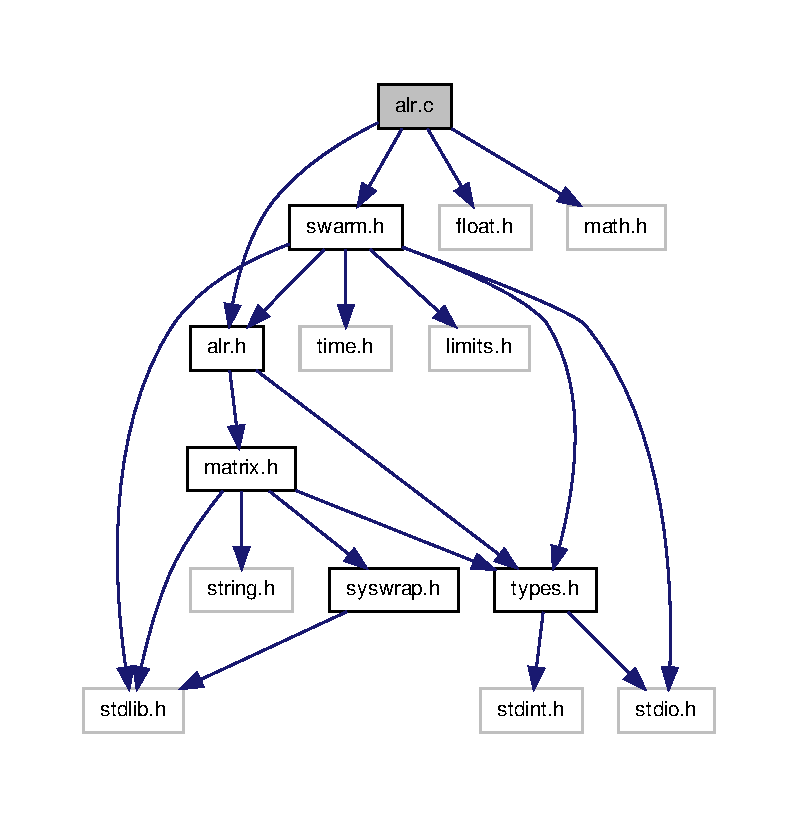
\includegraphics[width=350pt]{alr_8c__incl}
\end{center}
\end{figure}
\subsection*{Functions}
\begin{DoxyCompactItemize}
\item 
\hyperlink{types_8h_a7bc9d9790537ce02dc19f7fc4080b98b}{melem\-\_\-t} \hyperlink{alr_8c_a52e321cf23b59535e518c501e8b7be56}{min} (const \hyperlink{types_8h_a7bc9d9790537ce02dc19f7fc4080b98b}{melem\-\_\-t} v1, const \hyperlink{types_8h_a7bc9d9790537ce02dc19f7fc4080b98b}{melem\-\_\-t} v2)
\begin{DoxyCompactList}\small\item\em finds minimum from two specified values \end{DoxyCompactList}\item 
\hyperlink{types_8h_a7bc9d9790537ce02dc19f7fc4080b98b}{melem\-\_\-t} \hyperlink{alr_8c_acff303ddddc77a04eb6e8a0d48437cd0}{max} (const \hyperlink{types_8h_a170cb8b681dd48ced181eb10f1c5c7c8}{mvec1\-\_\-t} vec1, const \hyperlink{types_8h_a4717ab46b712567c1482ad0f5b910027}{msize\-\_\-t} size)
\begin{DoxyCompactList}\small\item\em finds maximum from the specified vector \end{DoxyCompactList}\item 
\hyperlink{types_8h_a7bc9d9790537ce02dc19f7fc4080b98b}{melem\-\_\-t} \hyperlink{alr_8c_af5df7647c80e69574495ad7833eb2795}{amin} (const \hyperlink{types_8h_a7bc9d9790537ce02dc19f7fc4080b98b}{melem\-\_\-t} v1, const \hyperlink{types_8h_a7bc9d9790537ce02dc19f7fc4080b98b}{melem\-\_\-t} v2)
\begin{DoxyCompactList}\small\item\em implementation of mul operator \end{DoxyCompactList}\item 
\hyperlink{types_8h_a7bc9d9790537ce02dc19f7fc4080b98b}{melem\-\_\-t} \hyperlink{alr_8c_ac811e294b5e0c0ba3db5eda36a24015e}{amax} (const \hyperlink{types_8h_a170cb8b681dd48ced181eb10f1c5c7c8}{mvec1\-\_\-t} vec1, const \hyperlink{types_8h_a4717ab46b712567c1482ad0f5b910027}{msize\-\_\-t} size)
\begin{DoxyCompactList}\small\item\em implementation of plus operator \end{DoxyCompactList}\item 
\hyperlink{types_8h_a9cf4b4aa35e29c0b7ac453f592d9bf84}{atm\-\_\-err\-\_\-code} \hyperlink{alr_8c_ada70870c4160d409463434090c089f03}{automata\-\_\-init} (\hyperlink{structautomata__t}{automata\-\_\-t} $\ast$atm, int is\-\_\-read, double max\-\_\-los, double min\-\_\-los, \hyperlink{types_8h_a9052d9742e283c5c2169b5b06f8245f0}{feat\-\_\-t} $\ast$min\-\_\-tab, \hyperlink{types_8h_a9052d9742e283c5c2169b5b06f8245f0}{feat\-\_\-t} $\ast$max\-\_\-tab, const \hyperlink{types_8h_a594c3568b9a4bfb59d5d849a52dd9fe0}{fsize\-\_\-t} feature\-\_\-num, const \hyperlink{types_8h_a4717ab46b712567c1482ad0f5b910027}{msize\-\_\-t} splits, const \hyperlink{types_8h_a4717ab46b712567c1482ad0f5b910027}{msize\-\_\-t} sym\-\_\-class\-\_\-num)
\begin{DoxyCompactList}\small\item\em Initializes automata instance. \end{DoxyCompactList}\item 
void \hyperlink{alr_8c_a6cf5da7c9a1427caebc7d9f01823a03a}{init\-\_\-from\-\_\-vec} (double $\ast$vec, \hyperlink{structautomata__t}{automata\-\_\-t} $\ast$atm, double nondet\-\_\-prop)
\begin{DoxyCompactList}\small\item\em Initializes the automata matrix (integers) from pso optimized data. \end{DoxyCompactList}\item 
void \hyperlink{alr_8c_a9d4a407471cd04d276f161516201c865}{init\-\_\-from\-\_\-dvec} (double $\ast$vec, \hyperlink{structautomata__t}{automata\-\_\-t} $\ast$atm)
\begin{DoxyCompactList}\small\item\em Initializes the automata matrix (doubles) from pso optimized data. \end{DoxyCompactList}\item 
void \hyperlink{alr_8c_a026778d0bf7e1d9ca1756d4ce5720960}{init\-\_\-from\-\_\-vec\-\_\-old} (double $\ast$vec, \hyperlink{structautomata__t}{automata\-\_\-t} $\ast$atm)
\item 
void \hyperlink{alr_8c_a28ad4c77e48247a022126cce1b61e78c}{automata\-\_\-free} (\hyperlink{structautomata__t}{automata\-\_\-t} $\ast$atm)
\begin{DoxyCompactList}\small\item\em Frees the memory. \end{DoxyCompactList}\item 
void \hyperlink{alr_8c_a11948aac5ae0674311c17f266183658f}{automata\-\_\-build} (double $\ast$vec, \hyperlink{structautomata__t}{automata\-\_\-t} $\ast$atm, \hyperlink{types_8h_a4717ab46b712567c1482ad0f5b910027}{msize\-\_\-t} input\-\_\-size, \hyperlink{structfeature__t}{feature\-\_\-t} $\ast$features, double $\ast$err\-\_\-num, double nondet\-\_\-prop)
\begin{DoxyCompactList}\small\item\em Starts building of the automata. \end{DoxyCompactList}\item 
\hyperlink{types_8h_a9cf4b4aa35e29c0b7ac453f592d9bf84}{atm\-\_\-err\-\_\-code} \hyperlink{alr_8c_a95c961e4fa720db406b761233fe7180d}{automata\-\_\-build\-\_\-start} (\hyperlink{structautomata__t}{automata\-\_\-t} $\ast$atm, \hyperlink{types_8h_a4717ab46b712567c1482ad0f5b910027}{msize\-\_\-t} input\-\_\-size, \hyperlink{structfeature__t}{feature\-\_\-t} $\ast$features, \hyperlink{types_8h_a4717ab46b712567c1482ad0f5b910027}{msize\-\_\-t} repeat)
\item 
\hyperlink{types_8h_a9cf4b4aa35e29c0b7ac453f592d9bf84}{atm\-\_\-err\-\_\-code} \hyperlink{alr_8c_acccf23fb33ef2ca8bd9afd1c743fadf5}{automata\-\_\-split\-\_\-range} (\hyperlink{structautomata__t}{automata\-\_\-t} $\ast$atm)
\begin{DoxyCompactList}\small\item\em Maps real values -\/$>$ \mbox{[}0..1\mbox{]}. \end{DoxyCompactList}\item 
\hyperlink{types_8h_a9cf4b4aa35e29c0b7ac453f592d9bf84}{atm\-\_\-err\-\_\-code} \hyperlink{alr_8c_a4337f015fab6adb23d38faae40cc378d}{automata\-\_\-init\-\_\-matrix} (\hyperlink{structautomata__t}{automata\-\_\-t} $\ast$atm)
\begin{DoxyCompactList}\small\item\em Initializes a matrix related with specified automata. \end{DoxyCompactList}\item 
\hyperlink{types_8h_af7ba14dcfbe385d9b130ff508c4e89b8}{ftr\-\_\-err\-\_\-code} \hyperlink{alr_8c_af56f4c4068fc82770bca730d045d5727}{automata\-\_\-feature\-\_\-normalize} (\hyperlink{structautomata__t}{automata\-\_\-t} $\ast$atm, \hyperlink{structfeature__t}{feature\-\_\-t} $\ast$feat)
\begin{DoxyCompactList}\small\item\em Responsible for normalizing specified feature vector. \end{DoxyCompactList}\item 
void \hyperlink{alr_8c_a41b4a4554ba45c4eddf5c20f8f48f2b9}{print\-\_\-atm} (\hyperlink{structautomata__t}{automata\-\_\-t} $\ast$atm)
\begin{DoxyCompactList}\small\item\em Printing the automata matrix. \end{DoxyCompactList}\end{DoxyCompactItemize}


\subsection{Function Documentation}
\hypertarget{alr_8c_ac811e294b5e0c0ba3db5eda36a24015e}{\index{alr.\-c@{alr.\-c}!amax@{amax}}
\index{amax@{amax}!alr.c@{alr.\-c}}
\subsubsection[{amax}]{\setlength{\rightskip}{0pt plus 5cm}{\bf melem\-\_\-t} amax (
\begin{DoxyParamCaption}
\item[{const {\bf mvec1\-\_\-t}}]{vec1, }
\item[{const {\bf msize\-\_\-t}}]{size}
\end{DoxyParamCaption}
)}}\label{alr_8c_ac811e294b5e0c0ba3db5eda36a24015e}


implementation of plus operator 


\begin{DoxyParams}{Parameters}
{\em vec1} & vector of elements \\
\hline
{\em size} & size of vector\\
\hline
\end{DoxyParams}
\begin{DoxyReturn}{Returns}
composition function result 
\end{DoxyReturn}


Definition at line 37 of file alr.\-c.



Here is the caller graph for this function\-:\nopagebreak
\begin{figure}[H]
\begin{center}
\leavevmode
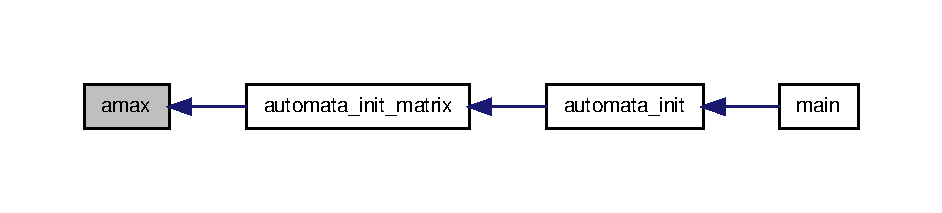
\includegraphics[width=350pt]{alr_8c_ac811e294b5e0c0ba3db5eda36a24015e_icgraph}
\end{center}
\end{figure}


\hypertarget{alr_8c_af5df7647c80e69574495ad7833eb2795}{\index{alr.\-c@{alr.\-c}!amin@{amin}}
\index{amin@{amin}!alr.c@{alr.\-c}}
\subsubsection[{amin}]{\setlength{\rightskip}{0pt plus 5cm}{\bf melem\-\_\-t} amin (
\begin{DoxyParamCaption}
\item[{const {\bf melem\-\_\-t}}]{v1, }
\item[{const {\bf melem\-\_\-t}}]{v2}
\end{DoxyParamCaption}
)}}\label{alr_8c_af5df7647c80e69574495ad7833eb2795}


implementation of mul operator 


\begin{DoxyParams}{Parameters}
{\em v1} & first value \\
\hline
{\em v2} & second value\\
\hline
\end{DoxyParams}
\begin{DoxyReturn}{Returns}
composition function result 
\end{DoxyReturn}


Definition at line 32 of file alr.\-c.



Here is the caller graph for this function\-:\nopagebreak
\begin{figure}[H]
\begin{center}
\leavevmode
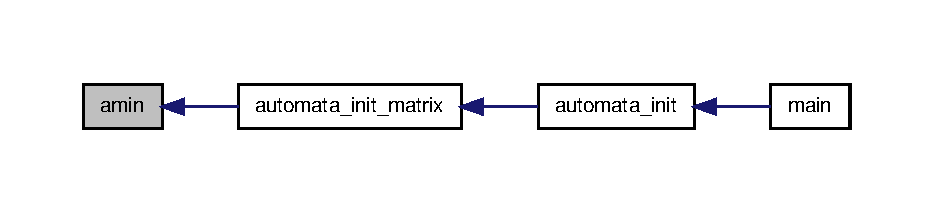
\includegraphics[width=350pt]{alr_8c_af5df7647c80e69574495ad7833eb2795_icgraph}
\end{center}
\end{figure}


\hypertarget{alr_8c_a11948aac5ae0674311c17f266183658f}{\index{alr.\-c@{alr.\-c}!automata\-\_\-build@{automata\-\_\-build}}
\index{automata\-\_\-build@{automata\-\_\-build}!alr.c@{alr.\-c}}
\subsubsection[{automata\-\_\-build}]{\setlength{\rightskip}{0pt plus 5cm}void automata\-\_\-build (
\begin{DoxyParamCaption}
\item[{double $\ast$}]{vec, }
\item[{{\bf automata\-\_\-t} $\ast$}]{atm, }
\item[{{\bf msize\-\_\-t}}]{input\-\_\-size, }
\item[{{\bf feature\-\_\-t} $\ast$}]{features, }
\item[{double $\ast$}]{err\-\_\-num, }
\item[{double}]{nondet\-\_\-prop}
\end{DoxyParamCaption}
)}}\label{alr_8c_a11948aac5ae0674311c17f266183658f}


Starts building of the automata. 


\begin{DoxyParams}{Parameters}
{\em vec,\-:} & Vector with data to initialize the automata matrix \\
\hline
{\em atm,\-:} & Automata \\
\hline
{\em input\-\_\-size,\-:} & Number of symbols to test \\
\hline
{\em features,\-:} & Vector of features \\
\hline
{\em err\-\_\-num,\-:} & Number of wrong recognized symbols \\
\hline
{\em nondet\-\_\-prop,\-:} & Nondeterministic automata percentage limit \\
\hline
\end{DoxyParams}


Definition at line 239 of file alr.\-c.



Here is the call graph for this function\-:\nopagebreak
\begin{figure}[H]
\begin{center}
\leavevmode
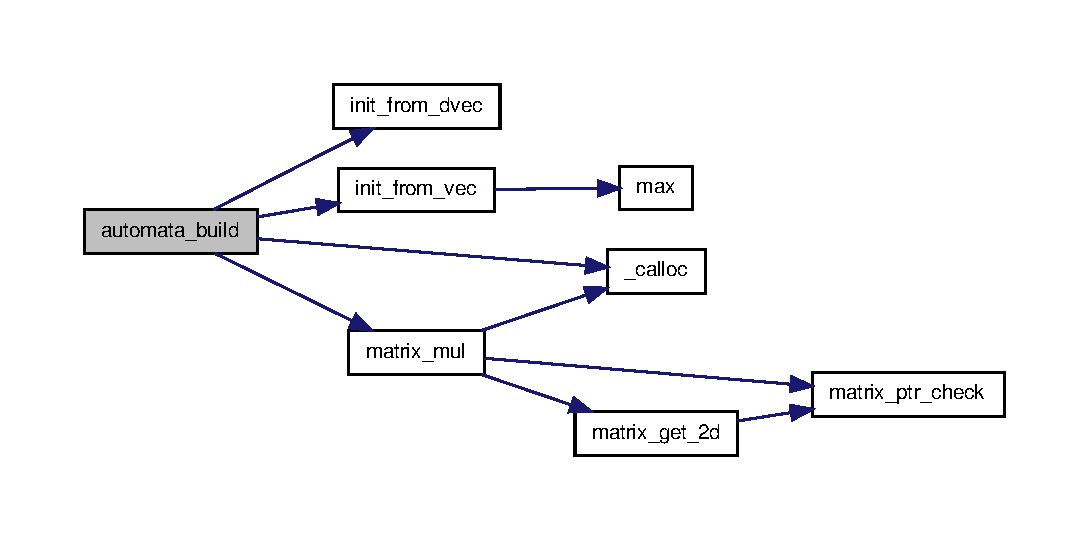
\includegraphics[width=350pt]{alr_8c_a11948aac5ae0674311c17f266183658f_cgraph}
\end{center}
\end{figure}




Here is the caller graph for this function\-:\nopagebreak
\begin{figure}[H]
\begin{center}
\leavevmode
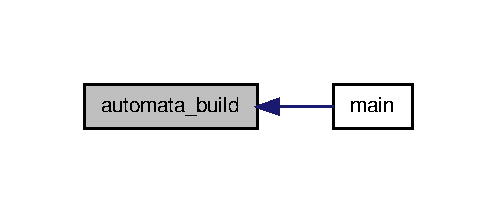
\includegraphics[width=238pt]{alr_8c_a11948aac5ae0674311c17f266183658f_icgraph}
\end{center}
\end{figure}


\hypertarget{alr_8c_a95c961e4fa720db406b761233fe7180d}{\index{alr.\-c@{alr.\-c}!automata\-\_\-build\-\_\-start@{automata\-\_\-build\-\_\-start}}
\index{automata\-\_\-build\-\_\-start@{automata\-\_\-build\-\_\-start}!alr.c@{alr.\-c}}
\subsubsection[{automata\-\_\-build\-\_\-start}]{\setlength{\rightskip}{0pt plus 5cm}{\bf atm\-\_\-err\-\_\-code} automata\-\_\-build\-\_\-start (
\begin{DoxyParamCaption}
\item[{{\bf automata\-\_\-t} $\ast$}]{atm, }
\item[{{\bf msize\-\_\-t}}]{input\-\_\-size, }
\item[{{\bf feature\-\_\-t} $\ast$}]{features, }
\item[{{\bf msize\-\_\-t}}]{repeat}
\end{DoxyParamCaption}
)}}\label{alr_8c_a95c961e4fa720db406b761233fe7180d}


Definition at line 385 of file alr.\-c.



Here is the call graph for this function\-:\nopagebreak
\begin{figure}[H]
\begin{center}
\leavevmode
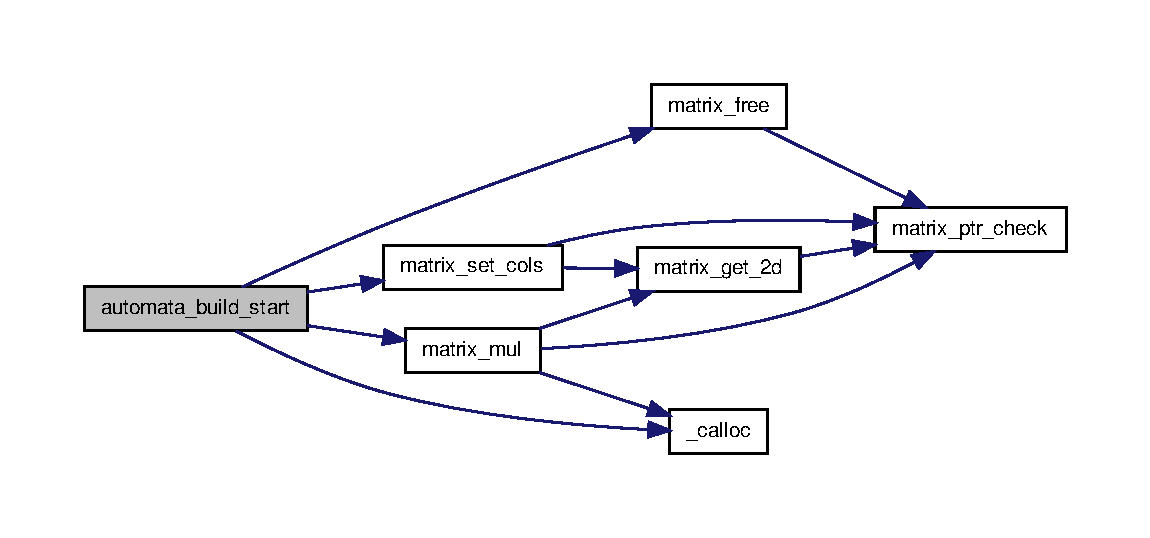
\includegraphics[width=350pt]{alr_8c_a95c961e4fa720db406b761233fe7180d_cgraph}
\end{center}
\end{figure}


\hypertarget{alr_8c_af56f4c4068fc82770bca730d045d5727}{\index{alr.\-c@{alr.\-c}!automata\-\_\-feature\-\_\-normalize@{automata\-\_\-feature\-\_\-normalize}}
\index{automata\-\_\-feature\-\_\-normalize@{automata\-\_\-feature\-\_\-normalize}!alr.c@{alr.\-c}}
\subsubsection[{automata\-\_\-feature\-\_\-normalize}]{\setlength{\rightskip}{0pt plus 5cm}{\bf ftr\-\_\-err\-\_\-code} automata\-\_\-feature\-\_\-normalize (
\begin{DoxyParamCaption}
\item[{{\bf automata\-\_\-t} $\ast$}]{atm, }
\item[{{\bf feature\-\_\-t} $\ast$}]{feat}
\end{DoxyParamCaption}
)}}\label{alr_8c_af56f4c4068fc82770bca730d045d5727}


Responsible for normalizing specified feature vector. 

F\-E\-A\-T\-U\-R\-E 
\begin{DoxyParams}{Parameters}
{\em atm,\-:} & Pointer to \hyperlink{structautomata__t}{automata\-\_\-t}\\
\hline
\end{DoxyParams}
\begin{DoxyReturn}{Returns}
A\-T\-M\-\_\-\-O\-K if function succeed, error code in other cases 
\end{DoxyReturn}


Definition at line 514 of file alr.\-c.



Here is the call graph for this function\-:\nopagebreak
\begin{figure}[H]
\begin{center}
\leavevmode
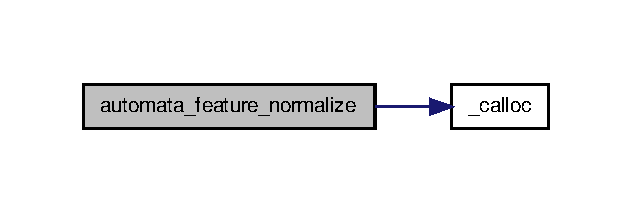
\includegraphics[width=304pt]{alr_8c_af56f4c4068fc82770bca730d045d5727_cgraph}
\end{center}
\end{figure}




Here is the caller graph for this function\-:\nopagebreak
\begin{figure}[H]
\begin{center}
\leavevmode
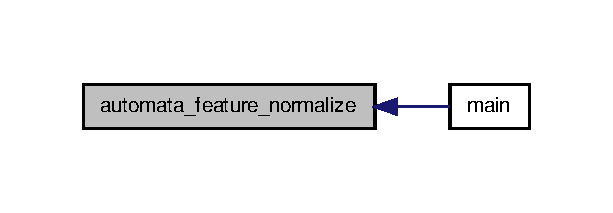
\includegraphics[width=294pt]{alr_8c_af56f4c4068fc82770bca730d045d5727_icgraph}
\end{center}
\end{figure}


\hypertarget{alr_8c_a28ad4c77e48247a022126cce1b61e78c}{\index{alr.\-c@{alr.\-c}!automata\-\_\-free@{automata\-\_\-free}}
\index{automata\-\_\-free@{automata\-\_\-free}!alr.c@{alr.\-c}}
\subsubsection[{automata\-\_\-free}]{\setlength{\rightskip}{0pt plus 5cm}void automata\-\_\-free (
\begin{DoxyParamCaption}
\item[{{\bf automata\-\_\-t} $\ast$}]{atm}
\end{DoxyParamCaption}
)}}\label{alr_8c_a28ad4c77e48247a022126cce1b61e78c}


Frees the memory. 


\begin{DoxyParams}{Parameters}
{\em atm,\-:} & Automata \\
\hline
\end{DoxyParams}


Definition at line 228 of file alr.\-c.



Here is the caller graph for this function\-:\nopagebreak
\begin{figure}[H]
\begin{center}
\leavevmode
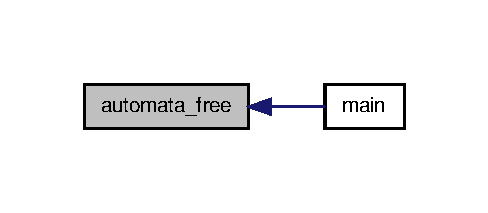
\includegraphics[width=234pt]{alr_8c_a28ad4c77e48247a022126cce1b61e78c_icgraph}
\end{center}
\end{figure}


\hypertarget{alr_8c_ada70870c4160d409463434090c089f03}{\index{alr.\-c@{alr.\-c}!automata\-\_\-init@{automata\-\_\-init}}
\index{automata\-\_\-init@{automata\-\_\-init}!alr.c@{alr.\-c}}
\subsubsection[{automata\-\_\-init}]{\setlength{\rightskip}{0pt plus 5cm}{\bf atm\-\_\-err\-\_\-code} automata\-\_\-init (
\begin{DoxyParamCaption}
\item[{{\bf automata\-\_\-t} $\ast$}]{atm, }
\item[{int}]{is\-\_\-read, }
\item[{double}]{max\-\_\-los, }
\item[{double}]{min\-\_\-los, }
\item[{{\bf feat\-\_\-t} $\ast$}]{min\-\_\-tab, }
\item[{{\bf feat\-\_\-t} $\ast$}]{max\-\_\-tab, }
\item[{const {\bf fsize\-\_\-t}}]{feature\-\_\-num, }
\item[{const {\bf msize\-\_\-t}}]{splits, }
\item[{const {\bf msize\-\_\-t}}]{sym\-\_\-class\-\_\-num}
\end{DoxyParamCaption}
)}}\label{alr_8c_ada70870c4160d409463434090c089f03}


Initializes automata instance. 

A\-U\-T\-O\-M\-A\-T\-A 
\begin{DoxyParams}{Parameters}
{\em atm,\-:} & Automata \\
\hline
{\em is\-\_\-read,\-:} & Is data read from file? \\
\hline
{\em max\-\_\-los,\-:} & Max value of generated feature \\
\hline
{\em min\-\_\-los,\-:} & Min value of generated feature \\
\hline
{\em min\-\_\-tab,\-:} & Min values of read features \\
\hline
{\em max\-\_\-tab,\-:} & Max values of read features \\
\hline
{\em feature\-\_\-num,\-:} & Number of features \\
\hline
{\em splits,\-:} & Number of \mbox{[}0..1\mbox{]} vector splits \\
\hline
{\em sym\-\_\-class\-\_\-num,\-:} & Number of symbols \\
\hline
\end{DoxyParams}
\begin{DoxyReturn}{Returns}

\end{DoxyReturn}


Definition at line 47 of file alr.\-c.



Here is the call graph for this function\-:\nopagebreak
\begin{figure}[H]
\begin{center}
\leavevmode
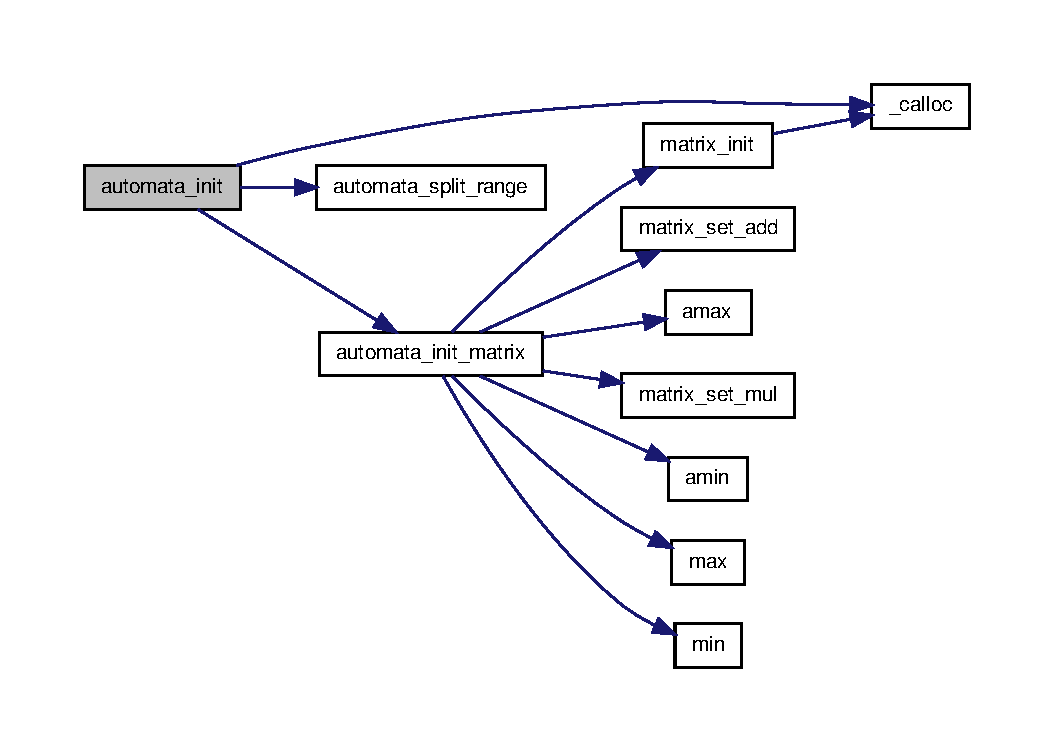
\includegraphics[width=350pt]{alr_8c_ada70870c4160d409463434090c089f03_cgraph}
\end{center}
\end{figure}




Here is the caller graph for this function\-:\nopagebreak
\begin{figure}[H]
\begin{center}
\leavevmode
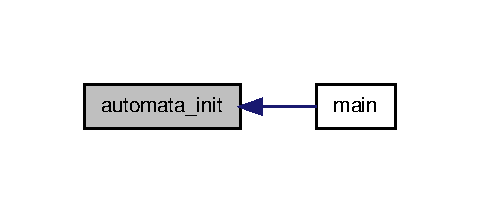
\includegraphics[width=230pt]{alr_8c_ada70870c4160d409463434090c089f03_icgraph}
\end{center}
\end{figure}


\hypertarget{alr_8c_a4337f015fab6adb23d38faae40cc378d}{\index{alr.\-c@{alr.\-c}!automata\-\_\-init\-\_\-matrix@{automata\-\_\-init\-\_\-matrix}}
\index{automata\-\_\-init\-\_\-matrix@{automata\-\_\-init\-\_\-matrix}!alr.c@{alr.\-c}}
\subsubsection[{automata\-\_\-init\-\_\-matrix}]{\setlength{\rightskip}{0pt plus 5cm}{\bf atm\-\_\-err\-\_\-code} automata\-\_\-init\-\_\-matrix (
\begin{DoxyParamCaption}
\item[{{\bf automata\-\_\-t} $\ast$}]{atm}
\end{DoxyParamCaption}
)}}\label{alr_8c_a4337f015fab6adb23d38faae40cc378d}


Initializes a matrix related with specified automata. 


\begin{DoxyParams}{Parameters}
{\em atm,\-:} & Pointer to \hyperlink{structautomata__t}{automata\-\_\-t}\\
\hline
\end{DoxyParams}
\begin{DoxyReturn}{Returns}
A\-T\-M\-\_\-\-O\-K if function succeed, error code in other cases 
\end{DoxyReturn}


Definition at line 457 of file alr.\-c.



Here is the call graph for this function\-:\nopagebreak
\begin{figure}[H]
\begin{center}
\leavevmode
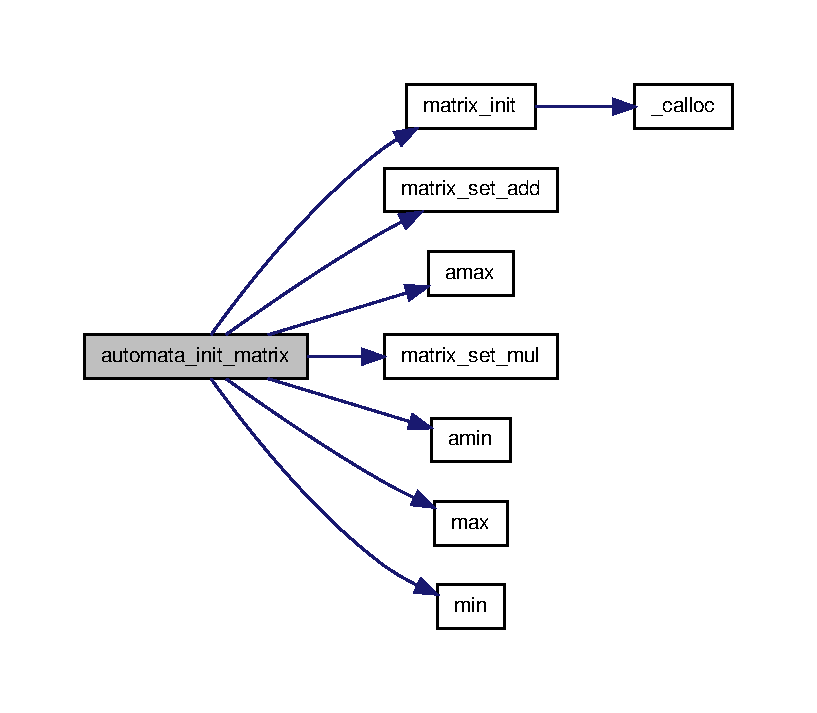
\includegraphics[width=350pt]{alr_8c_a4337f015fab6adb23d38faae40cc378d_cgraph}
\end{center}
\end{figure}




Here is the caller graph for this function\-:\nopagebreak
\begin{figure}[H]
\begin{center}
\leavevmode
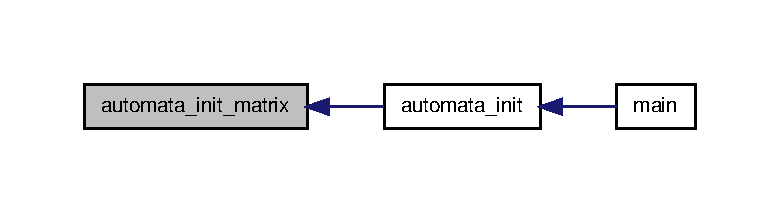
\includegraphics[width=350pt]{alr_8c_a4337f015fab6adb23d38faae40cc378d_icgraph}
\end{center}
\end{figure}


\hypertarget{alr_8c_acccf23fb33ef2ca8bd9afd1c743fadf5}{\index{alr.\-c@{alr.\-c}!automata\-\_\-split\-\_\-range@{automata\-\_\-split\-\_\-range}}
\index{automata\-\_\-split\-\_\-range@{automata\-\_\-split\-\_\-range}!alr.c@{alr.\-c}}
\subsubsection[{automata\-\_\-split\-\_\-range}]{\setlength{\rightskip}{0pt plus 5cm}{\bf atm\-\_\-err\-\_\-code} automata\-\_\-split\-\_\-range (
\begin{DoxyParamCaption}
\item[{{\bf automata\-\_\-t} $\ast$}]{atm}
\end{DoxyParamCaption}
)}}\label{alr_8c_acccf23fb33ef2ca8bd9afd1c743fadf5}


Maps real values -\/$>$ \mbox{[}0..1\mbox{]}. 


\begin{DoxyParams}{Parameters}
{\em atm,\-:} & Pointer to \hyperlink{structautomata__t}{automata\-\_\-t}\\
\hline
\end{DoxyParams}
\begin{DoxyReturn}{Returns}
A\-T\-M\-\_\-\-O\-K if function succeed, error code in other cases 
\end{DoxyReturn}


Definition at line 442 of file alr.\-c.



Here is the caller graph for this function\-:\nopagebreak
\begin{figure}[H]
\begin{center}
\leavevmode
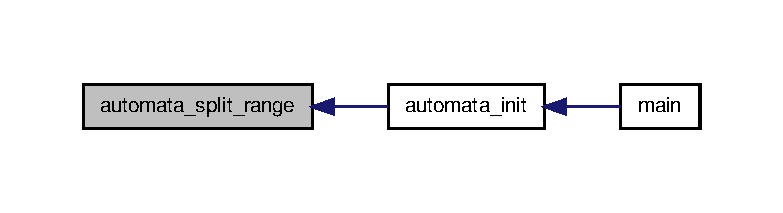
\includegraphics[width=350pt]{alr_8c_acccf23fb33ef2ca8bd9afd1c743fadf5_icgraph}
\end{center}
\end{figure}


\hypertarget{alr_8c_a9d4a407471cd04d276f161516201c865}{\index{alr.\-c@{alr.\-c}!init\-\_\-from\-\_\-dvec@{init\-\_\-from\-\_\-dvec}}
\index{init\-\_\-from\-\_\-dvec@{init\-\_\-from\-\_\-dvec}!alr.c@{alr.\-c}}
\subsubsection[{init\-\_\-from\-\_\-dvec}]{\setlength{\rightskip}{0pt plus 5cm}void init\-\_\-from\-\_\-dvec (
\begin{DoxyParamCaption}
\item[{double $\ast$}]{vec, }
\item[{{\bf automata\-\_\-t} $\ast$}]{atm}
\end{DoxyParamCaption}
)}}\label{alr_8c_a9d4a407471cd04d276f161516201c865}


Initializes the automata matrix (doubles) from pso optimized data. 


\begin{DoxyParams}{Parameters}
{\em vec,\-:} & P\-S\-O vector \\
\hline
{\em atm,\-:} & Automata \\
\hline
\end{DoxyParams}


Definition at line 177 of file alr.\-c.



Here is the caller graph for this function\-:\nopagebreak
\begin{figure}[H]
\begin{center}
\leavevmode
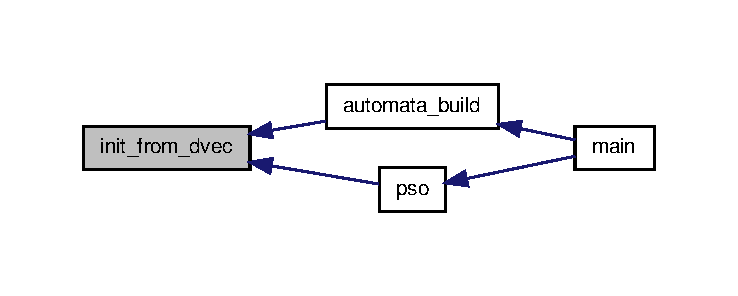
\includegraphics[width=350pt]{alr_8c_a9d4a407471cd04d276f161516201c865_icgraph}
\end{center}
\end{figure}


\hypertarget{alr_8c_a6cf5da7c9a1427caebc7d9f01823a03a}{\index{alr.\-c@{alr.\-c}!init\-\_\-from\-\_\-vec@{init\-\_\-from\-\_\-vec}}
\index{init\-\_\-from\-\_\-vec@{init\-\_\-from\-\_\-vec}!alr.c@{alr.\-c}}
\subsubsection[{init\-\_\-from\-\_\-vec}]{\setlength{\rightskip}{0pt plus 5cm}void init\-\_\-from\-\_\-vec (
\begin{DoxyParamCaption}
\item[{double $\ast$}]{vec, }
\item[{{\bf automata\-\_\-t} $\ast$}]{atm, }
\item[{double}]{nondet\-\_\-prop}
\end{DoxyParamCaption}
)}}\label{alr_8c_a6cf5da7c9a1427caebc7d9f01823a03a}


Initializes the automata matrix (integers) from pso optimized data. 


\begin{DoxyParams}{Parameters}
{\em vec,\-:} & P\-S\-O vector \\
\hline
{\em atm,\-:} & Automata \\
\hline
{\em nondet\-\_\-prop,\-:} & Nondeterministic automata percentage limit \\
\hline
\end{DoxyParams}


Definition at line 97 of file alr.\-c.



Here is the call graph for this function\-:\nopagebreak
\begin{figure}[H]
\begin{center}
\leavevmode
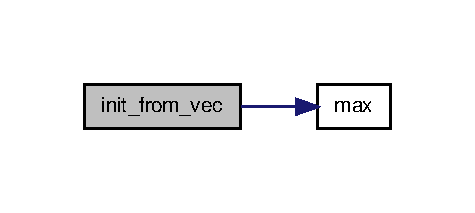
\includegraphics[width=228pt]{alr_8c_a6cf5da7c9a1427caebc7d9f01823a03a_cgraph}
\end{center}
\end{figure}




Here is the caller graph for this function\-:\nopagebreak
\begin{figure}[H]
\begin{center}
\leavevmode
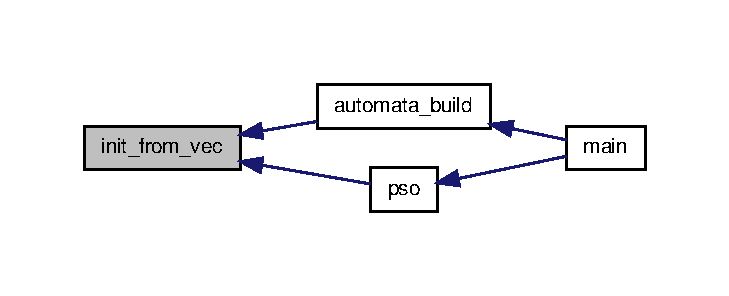
\includegraphics[width=350pt]{alr_8c_a6cf5da7c9a1427caebc7d9f01823a03a_icgraph}
\end{center}
\end{figure}


\hypertarget{alr_8c_a026778d0bf7e1d9ca1756d4ce5720960}{\index{alr.\-c@{alr.\-c}!init\-\_\-from\-\_\-vec\-\_\-old@{init\-\_\-from\-\_\-vec\-\_\-old}}
\index{init\-\_\-from\-\_\-vec\-\_\-old@{init\-\_\-from\-\_\-vec\-\_\-old}!alr.c@{alr.\-c}}
\subsubsection[{init\-\_\-from\-\_\-vec\-\_\-old}]{\setlength{\rightskip}{0pt plus 5cm}void init\-\_\-from\-\_\-vec\-\_\-old (
\begin{DoxyParamCaption}
\item[{double $\ast$}]{vec, }
\item[{{\bf automata\-\_\-t} $\ast$}]{atm}
\end{DoxyParamCaption}
)}}\label{alr_8c_a026778d0bf7e1d9ca1756d4ce5720960}


Definition at line 193 of file alr.\-c.



Here is the call graph for this function\-:\nopagebreak
\begin{figure}[H]
\begin{center}
\leavevmode
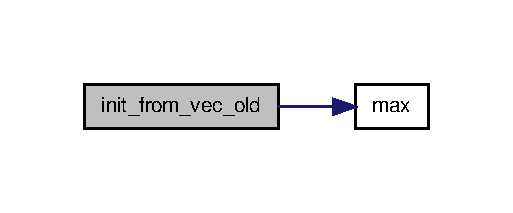
\includegraphics[width=246pt]{alr_8c_a026778d0bf7e1d9ca1756d4ce5720960_cgraph}
\end{center}
\end{figure}


\hypertarget{alr_8c_acff303ddddc77a04eb6e8a0d48437cd0}{\index{alr.\-c@{alr.\-c}!max@{max}}
\index{max@{max}!alr.c@{alr.\-c}}
\subsubsection[{max}]{\setlength{\rightskip}{0pt plus 5cm}{\bf melem\-\_\-t} max (
\begin{DoxyParamCaption}
\item[{const {\bf mvec1\-\_\-t}}]{vec1, }
\item[{const {\bf msize\-\_\-t}}]{size}
\end{DoxyParamCaption}
)}}\label{alr_8c_acff303ddddc77a04eb6e8a0d48437cd0}


finds maximum from the specified vector 


\begin{DoxyParams}{Parameters}
{\em vec1} & vector of elements \\
\hline
{\em size} & size of vector\\
\hline
\end{DoxyParams}
\begin{DoxyReturn}{Returns}
maximum value from vector 
\end{DoxyReturn}


Definition at line 13 of file alr.\-c.



Here is the caller graph for this function\-:\nopagebreak
\begin{figure}[H]
\begin{center}
\leavevmode
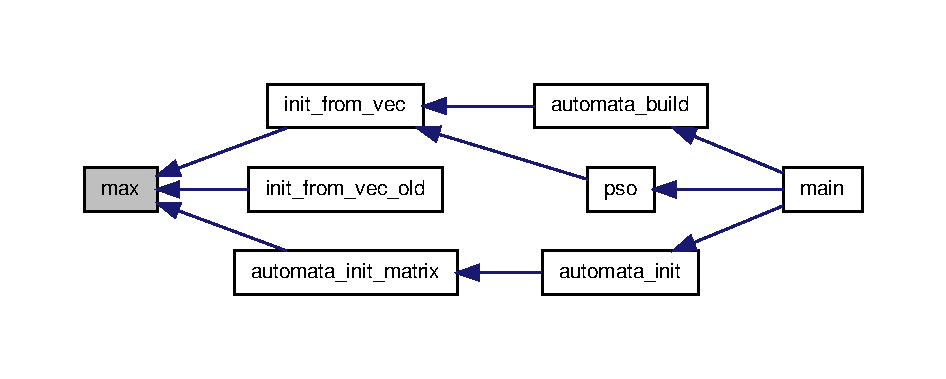
\includegraphics[width=350pt]{alr_8c_acff303ddddc77a04eb6e8a0d48437cd0_icgraph}
\end{center}
\end{figure}


\hypertarget{alr_8c_a52e321cf23b59535e518c501e8b7be56}{\index{alr.\-c@{alr.\-c}!min@{min}}
\index{min@{min}!alr.c@{alr.\-c}}
\subsubsection[{min}]{\setlength{\rightskip}{0pt plus 5cm}{\bf melem\-\_\-t} min (
\begin{DoxyParamCaption}
\item[{const {\bf melem\-\_\-t}}]{v1, }
\item[{const {\bf melem\-\_\-t}}]{v2}
\end{DoxyParamCaption}
)}}\label{alr_8c_a52e321cf23b59535e518c501e8b7be56}


finds minimum from two specified values 

M\-A\-T\-R\-I\-X A\-D\-D \& M\-U\-L F\-U\-N\-C 
\begin{DoxyParams}{Parameters}
{\em v1} & first value \\
\hline
{\em v2} & second value\\
\hline
\end{DoxyParams}
\begin{DoxyReturn}{Returns}
minimum from two values 
\end{DoxyReturn}


Definition at line 8 of file alr.\-c.



Here is the caller graph for this function\-:\nopagebreak
\begin{figure}[H]
\begin{center}
\leavevmode
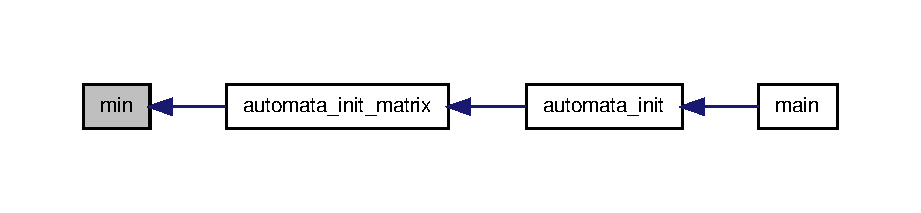
\includegraphics[width=350pt]{alr_8c_a52e321cf23b59535e518c501e8b7be56_icgraph}
\end{center}
\end{figure}


\hypertarget{alr_8c_a41b4a4554ba45c4eddf5c20f8f48f2b9}{\index{alr.\-c@{alr.\-c}!print\-\_\-atm@{print\-\_\-atm}}
\index{print\-\_\-atm@{print\-\_\-atm}!alr.c@{alr.\-c}}
\subsubsection[{print\-\_\-atm}]{\setlength{\rightskip}{0pt plus 5cm}void print\-\_\-atm (
\begin{DoxyParamCaption}
\item[{{\bf automata\-\_\-t} $\ast$}]{atm}
\end{DoxyParamCaption}
)}}\label{alr_8c_a41b4a4554ba45c4eddf5c20f8f48f2b9}


Printing the automata matrix. 


\begin{DoxyParams}{Parameters}
{\em atm,\-:} & Automata \\
\hline
\end{DoxyParams}


Definition at line 563 of file alr.\-c.


\hypertarget{alr_8h}{\section{alr.\-h File Reference}
\label{alr_8h}\index{alr.\-h@{alr.\-h}}
}
{\ttfamily \#include \char`\"{}types.\-h\char`\"{}}\\*
{\ttfamily \#include \char`\"{}matrix.\-h\char`\"{}}\\*
Include dependency graph for alr.\-h\-:\nopagebreak
\begin{figure}[H]
\begin{center}
\leavevmode
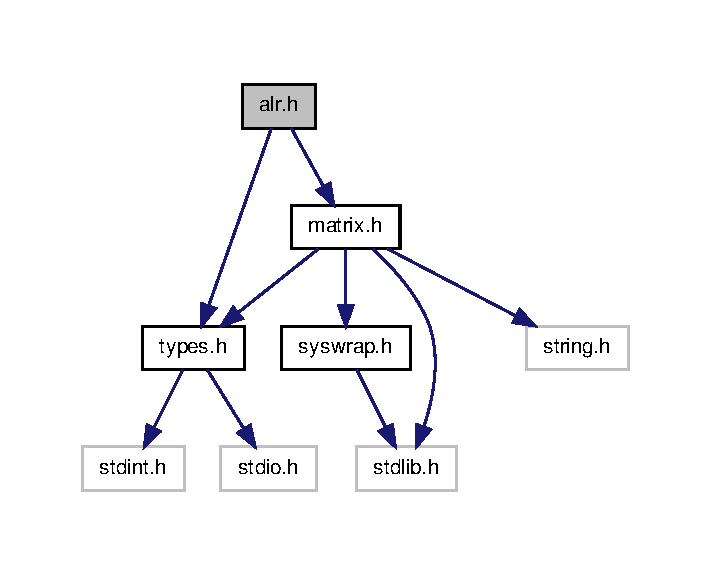
\includegraphics[width=341pt]{alr_8h__incl}
\end{center}
\end{figure}
This graph shows which files directly or indirectly include this file\-:\nopagebreak
\begin{figure}[H]
\begin{center}
\leavevmode
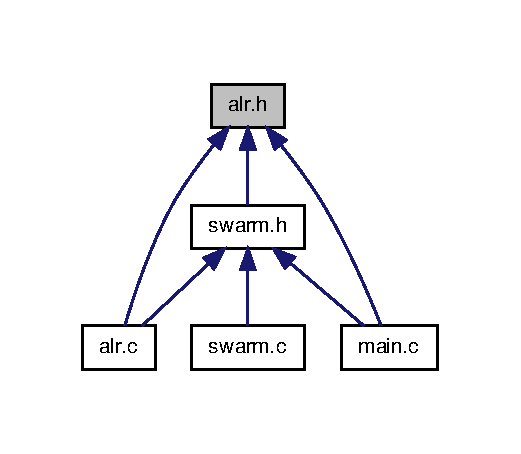
\includegraphics[width=250pt]{alr_8h__dep__incl}
\end{center}
\end{figure}
\subsection*{Data Structures}
\begin{DoxyCompactItemize}
\item 
struct \hyperlink{structfeature__t}{feature\-\_\-t}
\begin{DoxyCompactList}\small\item\em Structure that represents feature vector feat\-: Feature values vector size\-: Vector size correct\-: Correct state determin\-\_\-splits\-: Vector of deterministic splits A\-\_\-1, A\-\_\-3 .... A\-\_\-6, A\-\_\-2. \end{DoxyCompactList}\item 
struct \hyperlink{structstatistic__t}{statistic\-\_\-t}
\begin{DoxyCompactList}\small\item\em Structure that represents statistics of correctly distinguished symbols whole\-: Whole number of input features errors\-: Number of errors during the automata work fuzzy\-\_\-errors\-: Number of errors during the fuzzy automata work. \end{DoxyCompactList}\item 
struct \hyperlink{structautomata__t}{automata\-\_\-t}
\begin{DoxyCompactList}\small\item\em structure that represents dynamically generated automata feat\-: Feature structure mtx\-: Matrix structure stat\-: Statistic structure range\-: Range structure state\-: Current state splits\-: Number of splits on \mbox{[}0, 1\mbox{]} sym\-\_\-class\-\_\-num\-: Number of symbol classes max\-\_\-los\-: Max feature value of generated data min\-\_\-los\-: Min feature value of generated data min\-\_\-tab\-: Min feature values of read data max\-\_\-tab\-: Max feature values of read data is\-\_\-read\-: Is data read from files? fuzzy\-: Is automata fuzzy? \end{DoxyCompactList}\end{DoxyCompactItemize}
\subsection*{Functions}
\begin{DoxyCompactItemize}
\item 
\hyperlink{types_8h_a7bc9d9790537ce02dc19f7fc4080b98b}{melem\-\_\-t} \hyperlink{alr_8h_a52e321cf23b59535e518c501e8b7be56}{min} (const \hyperlink{types_8h_a7bc9d9790537ce02dc19f7fc4080b98b}{melem\-\_\-t} v1, const \hyperlink{types_8h_a7bc9d9790537ce02dc19f7fc4080b98b}{melem\-\_\-t} v2)
\begin{DoxyCompactList}\small\item\em finds minimum from two specified values \end{DoxyCompactList}\item 
\hyperlink{types_8h_a7bc9d9790537ce02dc19f7fc4080b98b}{melem\-\_\-t} \hyperlink{alr_8h_acff303ddddc77a04eb6e8a0d48437cd0}{max} (const \hyperlink{types_8h_a170cb8b681dd48ced181eb10f1c5c7c8}{mvec1\-\_\-t} vec1, const \hyperlink{types_8h_a4717ab46b712567c1482ad0f5b910027}{msize\-\_\-t} size)
\begin{DoxyCompactList}\small\item\em finds maximum from the specified vector \end{DoxyCompactList}\item 
\hyperlink{types_8h_a7bc9d9790537ce02dc19f7fc4080b98b}{melem\-\_\-t} \hyperlink{alr_8h_af5df7647c80e69574495ad7833eb2795}{amin} (const \hyperlink{types_8h_a7bc9d9790537ce02dc19f7fc4080b98b}{melem\-\_\-t} v1, const \hyperlink{types_8h_a7bc9d9790537ce02dc19f7fc4080b98b}{melem\-\_\-t} v2)
\begin{DoxyCompactList}\small\item\em implementation of mul operator \end{DoxyCompactList}\item 
\hyperlink{types_8h_a7bc9d9790537ce02dc19f7fc4080b98b}{melem\-\_\-t} \hyperlink{alr_8h_ac811e294b5e0c0ba3db5eda36a24015e}{amax} (const \hyperlink{types_8h_a170cb8b681dd48ced181eb10f1c5c7c8}{mvec1\-\_\-t} vec1, const \hyperlink{types_8h_a4717ab46b712567c1482ad0f5b910027}{msize\-\_\-t} size)
\begin{DoxyCompactList}\small\item\em implementation of plus operator \end{DoxyCompactList}\item 
\hyperlink{types_8h_a9cf4b4aa35e29c0b7ac453f592d9bf84}{atm\-\_\-err\-\_\-code} \hyperlink{alr_8h_ada70870c4160d409463434090c089f03}{automata\-\_\-init} (\hyperlink{structautomata__t}{automata\-\_\-t} $\ast$atm, int is\-\_\-read, double max\-\_\-los, double min\-\_\-los, \hyperlink{types_8h_a9052d9742e283c5c2169b5b06f8245f0}{feat\-\_\-t} $\ast$min\-\_\-tab, \hyperlink{types_8h_a9052d9742e283c5c2169b5b06f8245f0}{feat\-\_\-t} $\ast$max\-\_\-tab, const \hyperlink{types_8h_a594c3568b9a4bfb59d5d849a52dd9fe0}{fsize\-\_\-t} feature\-\_\-num, const \hyperlink{types_8h_a4717ab46b712567c1482ad0f5b910027}{msize\-\_\-t} splits, const \hyperlink{types_8h_a4717ab46b712567c1482ad0f5b910027}{msize\-\_\-t} sym\-\_\-class\-\_\-num)
\begin{DoxyCompactList}\small\item\em Initializes automata instance. \end{DoxyCompactList}\item 
void \hyperlink{alr_8h_a6cf5da7c9a1427caebc7d9f01823a03a}{init\-\_\-from\-\_\-vec} (double $\ast$vec, \hyperlink{structautomata__t}{automata\-\_\-t} $\ast$atm, double nondet\-\_\-prop)
\begin{DoxyCompactList}\small\item\em Initializes the automata matrix (integers) from pso optimized data. \end{DoxyCompactList}\item 
void \hyperlink{alr_8h_a9d4a407471cd04d276f161516201c865}{init\-\_\-from\-\_\-dvec} (double $\ast$vec, \hyperlink{structautomata__t}{automata\-\_\-t} $\ast$atm)
\begin{DoxyCompactList}\small\item\em Initializes the automata matrix (doubles) from pso optimized data. \end{DoxyCompactList}\item 
void \hyperlink{alr_8h_a28ad4c77e48247a022126cce1b61e78c}{automata\-\_\-free} (\hyperlink{structautomata__t}{automata\-\_\-t} $\ast$atm)
\begin{DoxyCompactList}\small\item\em Frees the memory. \end{DoxyCompactList}\item 
\hyperlink{types_8h_a9cf4b4aa35e29c0b7ac453f592d9bf84}{atm\-\_\-err\-\_\-code} \hyperlink{alr_8h_a4337f015fab6adb23d38faae40cc378d}{automata\-\_\-init\-\_\-matrix} (\hyperlink{structautomata__t}{automata\-\_\-t} $\ast$atm)
\begin{DoxyCompactList}\small\item\em Initializes a matrix related with specified automata. \end{DoxyCompactList}\item 
void \hyperlink{alr_8h_a11948aac5ae0674311c17f266183658f}{automata\-\_\-build} (double $\ast$vec, \hyperlink{structautomata__t}{automata\-\_\-t} $\ast$atm, \hyperlink{types_8h_a4717ab46b712567c1482ad0f5b910027}{msize\-\_\-t} input\-\_\-size, \hyperlink{structfeature__t}{feature\-\_\-t} $\ast$features, double $\ast$err\-\_\-num, double nondet\-\_\-prop)
\begin{DoxyCompactList}\small\item\em Starts building of the automata. \end{DoxyCompactList}\item 
\hyperlink{types_8h_a9cf4b4aa35e29c0b7ac453f592d9bf84}{atm\-\_\-err\-\_\-code} \hyperlink{alr_8h_acccf23fb33ef2ca8bd9afd1c743fadf5}{automata\-\_\-split\-\_\-range} (\hyperlink{structautomata__t}{automata\-\_\-t} $\ast$atm)
\begin{DoxyCompactList}\small\item\em Maps real values -\/$>$ \mbox{[}0..1\mbox{]}. \end{DoxyCompactList}\item 
\hyperlink{types_8h_af7ba14dcfbe385d9b130ff508c4e89b8}{ftr\-\_\-err\-\_\-code} \hyperlink{alr_8h_af56f4c4068fc82770bca730d045d5727}{automata\-\_\-feature\-\_\-normalize} (\hyperlink{structautomata__t}{automata\-\_\-t} $\ast$atm, \hyperlink{structfeature__t}{feature\-\_\-t} $\ast$feat)
\begin{DoxyCompactList}\small\item\em Responsible for normalizing specified feature vector. \end{DoxyCompactList}\item 
void \hyperlink{alr_8h_a41b4a4554ba45c4eddf5c20f8f48f2b9}{print\-\_\-atm} (\hyperlink{structautomata__t}{automata\-\_\-t} $\ast$atm)
\begin{DoxyCompactList}\small\item\em Printing the automata matrix. \end{DoxyCompactList}\end{DoxyCompactItemize}
\subsection*{Variables}
\begin{DoxyCompactItemize}
\item 
int \hyperlink{alr_8h_a52eec20db404060f6d759e455219ac67}{test\-\_\-run}
\end{DoxyCompactItemize}


\subsection{Function Documentation}
\hypertarget{alr_8h_ac811e294b5e0c0ba3db5eda36a24015e}{\index{alr.\-h@{alr.\-h}!amax@{amax}}
\index{amax@{amax}!alr.h@{alr.\-h}}
\subsubsection[{amax}]{\setlength{\rightskip}{0pt plus 5cm}{\bf melem\-\_\-t} amax (
\begin{DoxyParamCaption}
\item[{const {\bf mvec1\-\_\-t}}]{vec1, }
\item[{const {\bf msize\-\_\-t}}]{size}
\end{DoxyParamCaption}
)}}\label{alr_8h_ac811e294b5e0c0ba3db5eda36a24015e}


implementation of plus operator 


\begin{DoxyParams}{Parameters}
{\em vec1} & vector of elements \\
\hline
{\em size} & size of vector\\
\hline
\end{DoxyParams}
\begin{DoxyReturn}{Returns}
composition function result 
\end{DoxyReturn}


Definition at line 37 of file alr.\-c.



Here is the caller graph for this function\-:\nopagebreak
\begin{figure}[H]
\begin{center}
\leavevmode
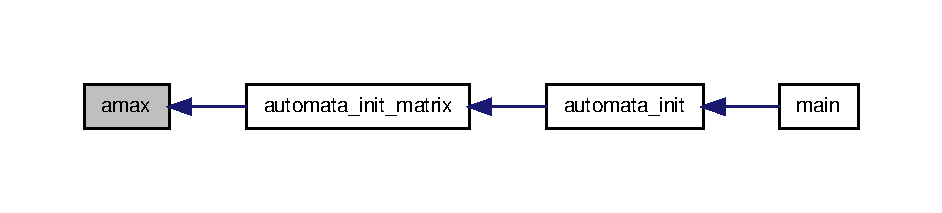
\includegraphics[width=350pt]{alr_8h_ac811e294b5e0c0ba3db5eda36a24015e_icgraph}
\end{center}
\end{figure}


\hypertarget{alr_8h_af5df7647c80e69574495ad7833eb2795}{\index{alr.\-h@{alr.\-h}!amin@{amin}}
\index{amin@{amin}!alr.h@{alr.\-h}}
\subsubsection[{amin}]{\setlength{\rightskip}{0pt plus 5cm}{\bf melem\-\_\-t} amin (
\begin{DoxyParamCaption}
\item[{const {\bf melem\-\_\-t}}]{v1, }
\item[{const {\bf melem\-\_\-t}}]{v2}
\end{DoxyParamCaption}
)}}\label{alr_8h_af5df7647c80e69574495ad7833eb2795}


implementation of mul operator 


\begin{DoxyParams}{Parameters}
{\em v1} & first value \\
\hline
{\em v2} & second value\\
\hline
\end{DoxyParams}
\begin{DoxyReturn}{Returns}
composition function result 
\end{DoxyReturn}


Definition at line 32 of file alr.\-c.



Here is the caller graph for this function\-:\nopagebreak
\begin{figure}[H]
\begin{center}
\leavevmode
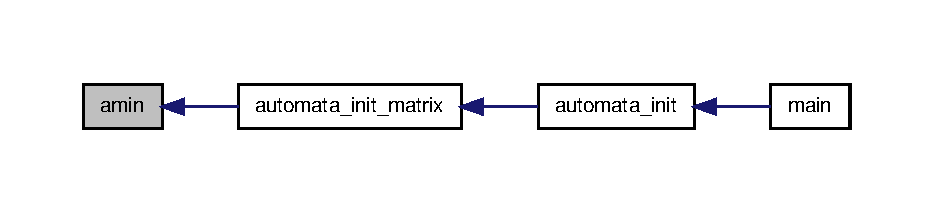
\includegraphics[width=350pt]{alr_8h_af5df7647c80e69574495ad7833eb2795_icgraph}
\end{center}
\end{figure}


\hypertarget{alr_8h_a11948aac5ae0674311c17f266183658f}{\index{alr.\-h@{alr.\-h}!automata\-\_\-build@{automata\-\_\-build}}
\index{automata\-\_\-build@{automata\-\_\-build}!alr.h@{alr.\-h}}
\subsubsection[{automata\-\_\-build}]{\setlength{\rightskip}{0pt plus 5cm}void automata\-\_\-build (
\begin{DoxyParamCaption}
\item[{double $\ast$}]{vec, }
\item[{{\bf automata\-\_\-t} $\ast$}]{atm, }
\item[{{\bf msize\-\_\-t}}]{input\-\_\-size, }
\item[{{\bf feature\-\_\-t} $\ast$}]{features, }
\item[{double $\ast$}]{err\-\_\-num, }
\item[{double}]{nondet\-\_\-prop}
\end{DoxyParamCaption}
)}}\label{alr_8h_a11948aac5ae0674311c17f266183658f}


Starts building of the automata. 


\begin{DoxyParams}{Parameters}
{\em vec,\-:} & Vector with data to initialize the automata matrix \\
\hline
{\em atm,\-:} & Automata \\
\hline
{\em input\-\_\-size,\-:} & Number of symbols to test \\
\hline
{\em features,\-:} & Vector of features \\
\hline
{\em err\-\_\-num,\-:} & Number of wrong recognized symbols \\
\hline
{\em nondet\-\_\-prop,\-:} & Nondeterministic automata percentage limit \\
\hline
\end{DoxyParams}


Definition at line 239 of file alr.\-c.



Here is the call graph for this function\-:\nopagebreak
\begin{figure}[H]
\begin{center}
\leavevmode
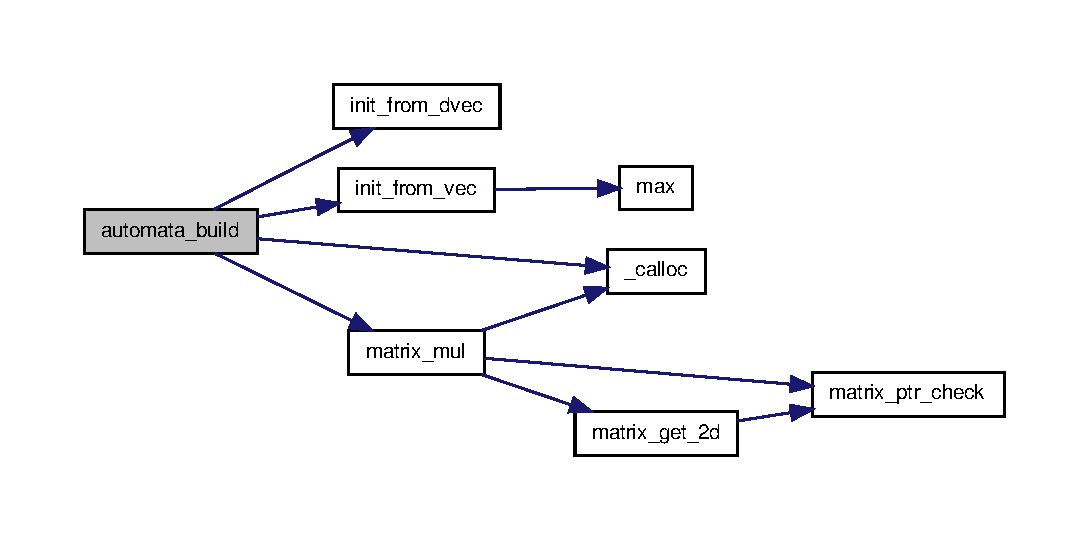
\includegraphics[width=350pt]{alr_8h_a11948aac5ae0674311c17f266183658f_cgraph}
\end{center}
\end{figure}




Here is the caller graph for this function\-:\nopagebreak
\begin{figure}[H]
\begin{center}
\leavevmode
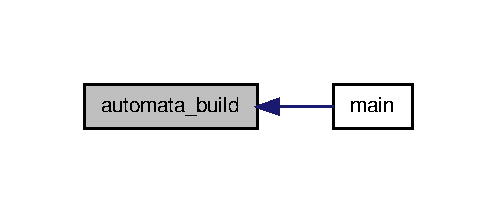
\includegraphics[width=238pt]{alr_8h_a11948aac5ae0674311c17f266183658f_icgraph}
\end{center}
\end{figure}


\hypertarget{alr_8h_af56f4c4068fc82770bca730d045d5727}{\index{alr.\-h@{alr.\-h}!automata\-\_\-feature\-\_\-normalize@{automata\-\_\-feature\-\_\-normalize}}
\index{automata\-\_\-feature\-\_\-normalize@{automata\-\_\-feature\-\_\-normalize}!alr.h@{alr.\-h}}
\subsubsection[{automata\-\_\-feature\-\_\-normalize}]{\setlength{\rightskip}{0pt plus 5cm}{\bf ftr\-\_\-err\-\_\-code} automata\-\_\-feature\-\_\-normalize (
\begin{DoxyParamCaption}
\item[{{\bf automata\-\_\-t} $\ast$}]{atm, }
\item[{{\bf feature\-\_\-t} $\ast$}]{feat}
\end{DoxyParamCaption}
)}}\label{alr_8h_af56f4c4068fc82770bca730d045d5727}


Responsible for normalizing specified feature vector. 

F\-E\-A\-T\-U\-R\-E 
\begin{DoxyParams}{Parameters}
{\em atm,\-:} & Pointer to \hyperlink{structautomata__t}{automata\-\_\-t}\\
\hline
\end{DoxyParams}
\begin{DoxyReturn}{Returns}
A\-T\-M\-\_\-\-O\-K if function succeed, error code in other cases 
\end{DoxyReturn}


Definition at line 514 of file alr.\-c.



Here is the call graph for this function\-:\nopagebreak
\begin{figure}[H]
\begin{center}
\leavevmode
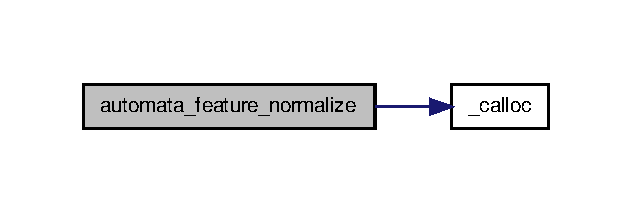
\includegraphics[width=304pt]{alr_8h_af56f4c4068fc82770bca730d045d5727_cgraph}
\end{center}
\end{figure}




Here is the caller graph for this function\-:\nopagebreak
\begin{figure}[H]
\begin{center}
\leavevmode
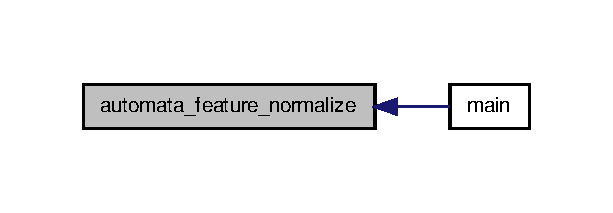
\includegraphics[width=294pt]{alr_8h_af56f4c4068fc82770bca730d045d5727_icgraph}
\end{center}
\end{figure}


\hypertarget{alr_8h_a28ad4c77e48247a022126cce1b61e78c}{\index{alr.\-h@{alr.\-h}!automata\-\_\-free@{automata\-\_\-free}}
\index{automata\-\_\-free@{automata\-\_\-free}!alr.h@{alr.\-h}}
\subsubsection[{automata\-\_\-free}]{\setlength{\rightskip}{0pt plus 5cm}void automata\-\_\-free (
\begin{DoxyParamCaption}
\item[{{\bf automata\-\_\-t} $\ast$}]{atm}
\end{DoxyParamCaption}
)}}\label{alr_8h_a28ad4c77e48247a022126cce1b61e78c}


Frees the memory. 


\begin{DoxyParams}{Parameters}
{\em atm,\-:} & Automata \\
\hline
\end{DoxyParams}


Definition at line 228 of file alr.\-c.



Here is the caller graph for this function\-:\nopagebreak
\begin{figure}[H]
\begin{center}
\leavevmode
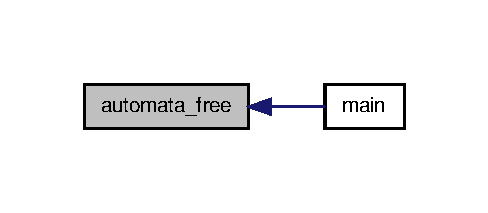
\includegraphics[width=234pt]{alr_8h_a28ad4c77e48247a022126cce1b61e78c_icgraph}
\end{center}
\end{figure}


\hypertarget{alr_8h_ada70870c4160d409463434090c089f03}{\index{alr.\-h@{alr.\-h}!automata\-\_\-init@{automata\-\_\-init}}
\index{automata\-\_\-init@{automata\-\_\-init}!alr.h@{alr.\-h}}
\subsubsection[{automata\-\_\-init}]{\setlength{\rightskip}{0pt plus 5cm}{\bf atm\-\_\-err\-\_\-code} automata\-\_\-init (
\begin{DoxyParamCaption}
\item[{{\bf automata\-\_\-t} $\ast$}]{atm, }
\item[{int}]{is\-\_\-read, }
\item[{double}]{max\-\_\-los, }
\item[{double}]{min\-\_\-los, }
\item[{{\bf feat\-\_\-t} $\ast$}]{min\-\_\-tab, }
\item[{{\bf feat\-\_\-t} $\ast$}]{max\-\_\-tab, }
\item[{const {\bf fsize\-\_\-t}}]{feature\-\_\-num, }
\item[{const {\bf msize\-\_\-t}}]{splits, }
\item[{const {\bf msize\-\_\-t}}]{sym\-\_\-class\-\_\-num}
\end{DoxyParamCaption}
)}}\label{alr_8h_ada70870c4160d409463434090c089f03}


Initializes automata instance. 

A\-U\-T\-O\-M\-A\-T\-A 
\begin{DoxyParams}{Parameters}
{\em atm,\-:} & Automata \\
\hline
{\em is\-\_\-read,\-:} & Is data read from file? \\
\hline
{\em max\-\_\-los,\-:} & Max value of generated feature \\
\hline
{\em min\-\_\-los,\-:} & Min value of generated feature \\
\hline
{\em min\-\_\-tab,\-:} & Min values of read features \\
\hline
{\em max\-\_\-tab,\-:} & Max values of read features \\
\hline
{\em feature\-\_\-num,\-:} & Number of features \\
\hline
{\em splits,\-:} & Number of \mbox{[}0..1\mbox{]} vector splits \\
\hline
{\em sym\-\_\-class\-\_\-num,\-:} & Number of symbols \\
\hline
\end{DoxyParams}
\begin{DoxyReturn}{Returns}

\end{DoxyReturn}


Definition at line 47 of file alr.\-c.



Here is the call graph for this function\-:\nopagebreak
\begin{figure}[H]
\begin{center}
\leavevmode
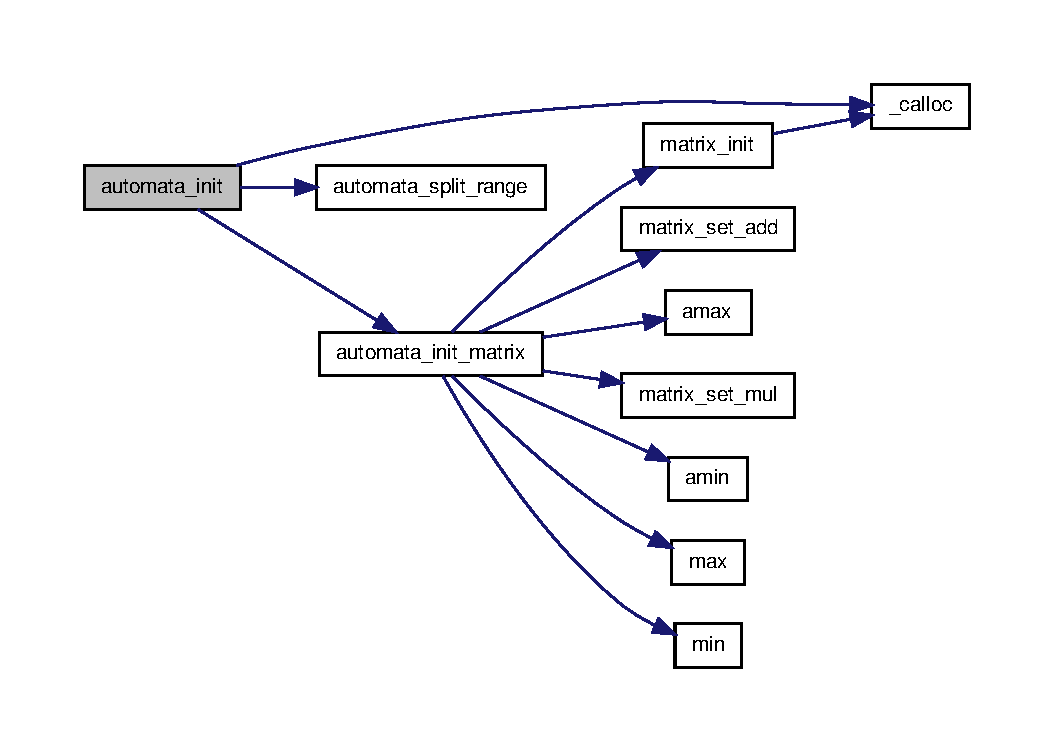
\includegraphics[width=350pt]{alr_8h_ada70870c4160d409463434090c089f03_cgraph}
\end{center}
\end{figure}




Here is the caller graph for this function\-:\nopagebreak
\begin{figure}[H]
\begin{center}
\leavevmode
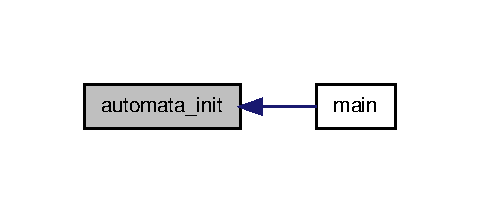
\includegraphics[width=230pt]{alr_8h_ada70870c4160d409463434090c089f03_icgraph}
\end{center}
\end{figure}


\hypertarget{alr_8h_a4337f015fab6adb23d38faae40cc378d}{\index{alr.\-h@{alr.\-h}!automata\-\_\-init\-\_\-matrix@{automata\-\_\-init\-\_\-matrix}}
\index{automata\-\_\-init\-\_\-matrix@{automata\-\_\-init\-\_\-matrix}!alr.h@{alr.\-h}}
\subsubsection[{automata\-\_\-init\-\_\-matrix}]{\setlength{\rightskip}{0pt plus 5cm}{\bf atm\-\_\-err\-\_\-code} automata\-\_\-init\-\_\-matrix (
\begin{DoxyParamCaption}
\item[{{\bf automata\-\_\-t} $\ast$}]{atm}
\end{DoxyParamCaption}
)}}\label{alr_8h_a4337f015fab6adb23d38faae40cc378d}


Initializes a matrix related with specified automata. 


\begin{DoxyParams}{Parameters}
{\em atm,\-:} & Pointer to \hyperlink{structautomata__t}{automata\-\_\-t}\\
\hline
\end{DoxyParams}
\begin{DoxyReturn}{Returns}
A\-T\-M\-\_\-\-O\-K if function succeed, error code in other cases 
\end{DoxyReturn}


Definition at line 457 of file alr.\-c.



Here is the call graph for this function\-:\nopagebreak
\begin{figure}[H]
\begin{center}
\leavevmode
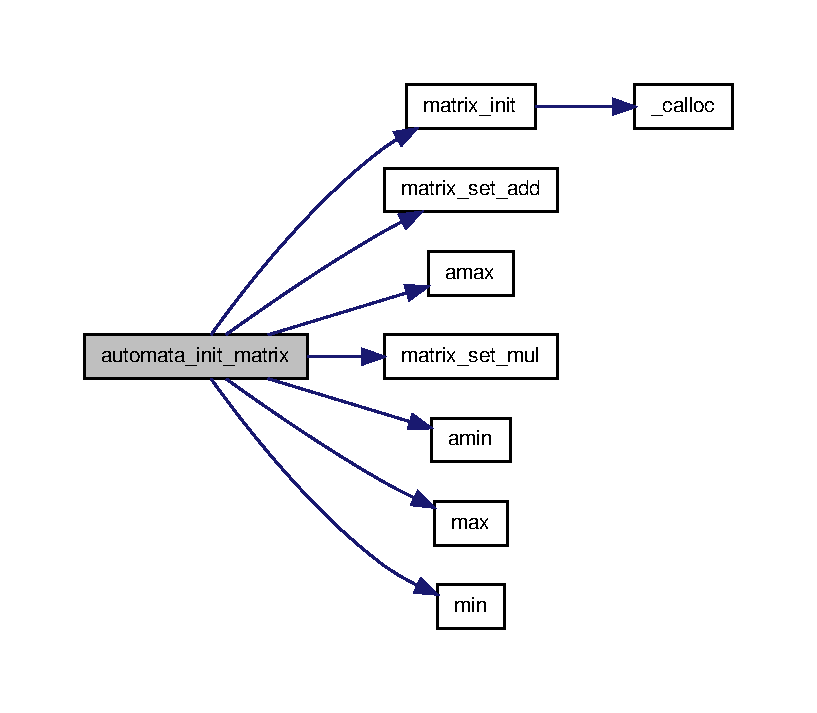
\includegraphics[width=350pt]{alr_8h_a4337f015fab6adb23d38faae40cc378d_cgraph}
\end{center}
\end{figure}




Here is the caller graph for this function\-:\nopagebreak
\begin{figure}[H]
\begin{center}
\leavevmode
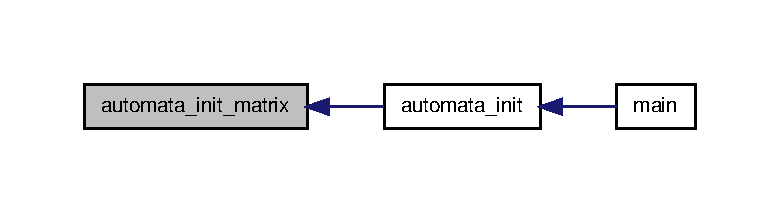
\includegraphics[width=350pt]{alr_8h_a4337f015fab6adb23d38faae40cc378d_icgraph}
\end{center}
\end{figure}


\hypertarget{alr_8h_acccf23fb33ef2ca8bd9afd1c743fadf5}{\index{alr.\-h@{alr.\-h}!automata\-\_\-split\-\_\-range@{automata\-\_\-split\-\_\-range}}
\index{automata\-\_\-split\-\_\-range@{automata\-\_\-split\-\_\-range}!alr.h@{alr.\-h}}
\subsubsection[{automata\-\_\-split\-\_\-range}]{\setlength{\rightskip}{0pt plus 5cm}{\bf atm\-\_\-err\-\_\-code} automata\-\_\-split\-\_\-range (
\begin{DoxyParamCaption}
\item[{{\bf automata\-\_\-t} $\ast$}]{atm}
\end{DoxyParamCaption}
)}}\label{alr_8h_acccf23fb33ef2ca8bd9afd1c743fadf5}


Maps real values -\/$>$ \mbox{[}0..1\mbox{]}. 


\begin{DoxyParams}{Parameters}
{\em atm,\-:} & Pointer to \hyperlink{structautomata__t}{automata\-\_\-t}\\
\hline
\end{DoxyParams}
\begin{DoxyReturn}{Returns}
A\-T\-M\-\_\-\-O\-K if function succeed, error code in other cases 
\end{DoxyReturn}


Definition at line 442 of file alr.\-c.



Here is the caller graph for this function\-:\nopagebreak
\begin{figure}[H]
\begin{center}
\leavevmode
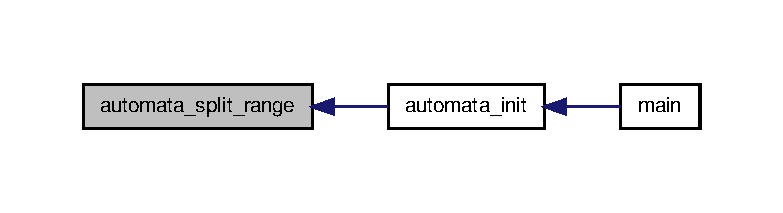
\includegraphics[width=350pt]{alr_8h_acccf23fb33ef2ca8bd9afd1c743fadf5_icgraph}
\end{center}
\end{figure}


\hypertarget{alr_8h_a9d4a407471cd04d276f161516201c865}{\index{alr.\-h@{alr.\-h}!init\-\_\-from\-\_\-dvec@{init\-\_\-from\-\_\-dvec}}
\index{init\-\_\-from\-\_\-dvec@{init\-\_\-from\-\_\-dvec}!alr.h@{alr.\-h}}
\subsubsection[{init\-\_\-from\-\_\-dvec}]{\setlength{\rightskip}{0pt plus 5cm}void init\-\_\-from\-\_\-dvec (
\begin{DoxyParamCaption}
\item[{double $\ast$}]{vec, }
\item[{{\bf automata\-\_\-t} $\ast$}]{atm}
\end{DoxyParamCaption}
)}}\label{alr_8h_a9d4a407471cd04d276f161516201c865}


Initializes the automata matrix (doubles) from pso optimized data. 


\begin{DoxyParams}{Parameters}
{\em vec,\-:} & P\-S\-O vector \\
\hline
{\em atm,\-:} & Automata \\
\hline
\end{DoxyParams}


Definition at line 177 of file alr.\-c.



Here is the caller graph for this function\-:\nopagebreak
\begin{figure}[H]
\begin{center}
\leavevmode
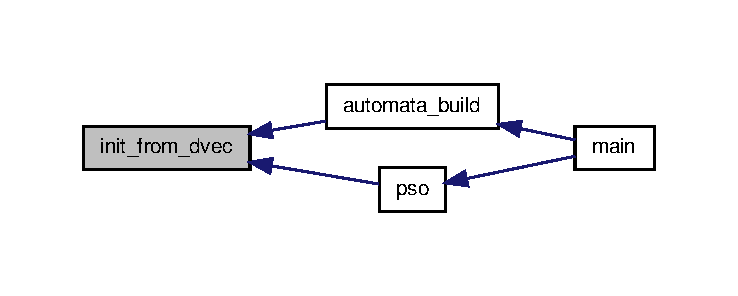
\includegraphics[width=350pt]{alr_8h_a9d4a407471cd04d276f161516201c865_icgraph}
\end{center}
\end{figure}


\hypertarget{alr_8h_a6cf5da7c9a1427caebc7d9f01823a03a}{\index{alr.\-h@{alr.\-h}!init\-\_\-from\-\_\-vec@{init\-\_\-from\-\_\-vec}}
\index{init\-\_\-from\-\_\-vec@{init\-\_\-from\-\_\-vec}!alr.h@{alr.\-h}}
\subsubsection[{init\-\_\-from\-\_\-vec}]{\setlength{\rightskip}{0pt plus 5cm}void init\-\_\-from\-\_\-vec (
\begin{DoxyParamCaption}
\item[{double $\ast$}]{vec, }
\item[{{\bf automata\-\_\-t} $\ast$}]{atm, }
\item[{double}]{nondet\-\_\-prop}
\end{DoxyParamCaption}
)}}\label{alr_8h_a6cf5da7c9a1427caebc7d9f01823a03a}


Initializes the automata matrix (integers) from pso optimized data. 


\begin{DoxyParams}{Parameters}
{\em vec,\-:} & P\-S\-O vector \\
\hline
{\em atm,\-:} & Automata \\
\hline
{\em nondet\-\_\-prop,\-:} & Nondeterministic automata percentage limit \\
\hline
\end{DoxyParams}


Definition at line 97 of file alr.\-c.



Here is the call graph for this function\-:\nopagebreak
\begin{figure}[H]
\begin{center}
\leavevmode
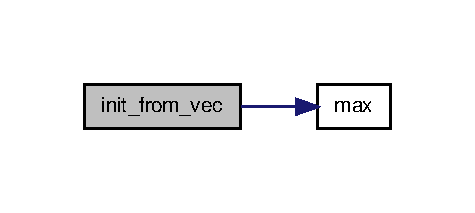
\includegraphics[width=228pt]{alr_8h_a6cf5da7c9a1427caebc7d9f01823a03a_cgraph}
\end{center}
\end{figure}




Here is the caller graph for this function\-:\nopagebreak
\begin{figure}[H]
\begin{center}
\leavevmode
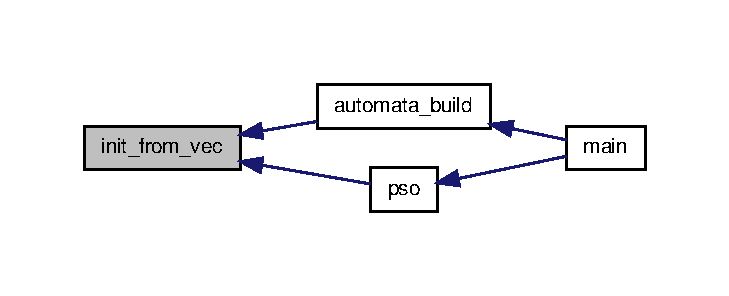
\includegraphics[width=350pt]{alr_8h_a6cf5da7c9a1427caebc7d9f01823a03a_icgraph}
\end{center}
\end{figure}


\hypertarget{alr_8h_acff303ddddc77a04eb6e8a0d48437cd0}{\index{alr.\-h@{alr.\-h}!max@{max}}
\index{max@{max}!alr.h@{alr.\-h}}
\subsubsection[{max}]{\setlength{\rightskip}{0pt plus 5cm}{\bf melem\-\_\-t} max (
\begin{DoxyParamCaption}
\item[{const {\bf mvec1\-\_\-t}}]{vec1, }
\item[{const {\bf msize\-\_\-t}}]{size}
\end{DoxyParamCaption}
)}}\label{alr_8h_acff303ddddc77a04eb6e8a0d48437cd0}


finds maximum from the specified vector 


\begin{DoxyParams}{Parameters}
{\em vec1} & vector of elements \\
\hline
{\em size} & size of vector\\
\hline
\end{DoxyParams}
\begin{DoxyReturn}{Returns}
maximum value from vector 
\end{DoxyReturn}


Definition at line 13 of file alr.\-c.



Here is the caller graph for this function\-:\nopagebreak
\begin{figure}[H]
\begin{center}
\leavevmode
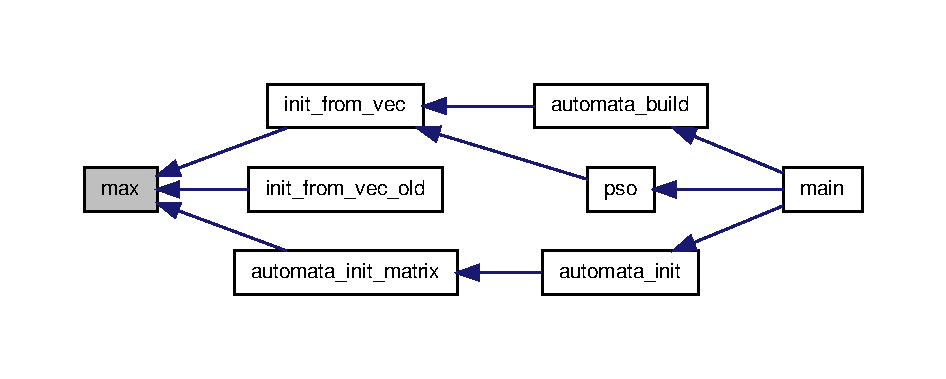
\includegraphics[width=350pt]{alr_8h_acff303ddddc77a04eb6e8a0d48437cd0_icgraph}
\end{center}
\end{figure}


\hypertarget{alr_8h_a52e321cf23b59535e518c501e8b7be56}{\index{alr.\-h@{alr.\-h}!min@{min}}
\index{min@{min}!alr.h@{alr.\-h}}
\subsubsection[{min}]{\setlength{\rightskip}{0pt plus 5cm}{\bf melem\-\_\-t} min (
\begin{DoxyParamCaption}
\item[{const {\bf melem\-\_\-t}}]{v1, }
\item[{const {\bf melem\-\_\-t}}]{v2}
\end{DoxyParamCaption}
)}}\label{alr_8h_a52e321cf23b59535e518c501e8b7be56}


finds minimum from two specified values 

M\-A\-T\-R\-I\-X A\-D\-D \& M\-U\-L F\-U\-N\-C 
\begin{DoxyParams}{Parameters}
{\em v1} & first value \\
\hline
{\em v2} & second value\\
\hline
\end{DoxyParams}
\begin{DoxyReturn}{Returns}
minimum from two values 
\end{DoxyReturn}


Definition at line 8 of file alr.\-c.



Here is the caller graph for this function\-:\nopagebreak
\begin{figure}[H]
\begin{center}
\leavevmode
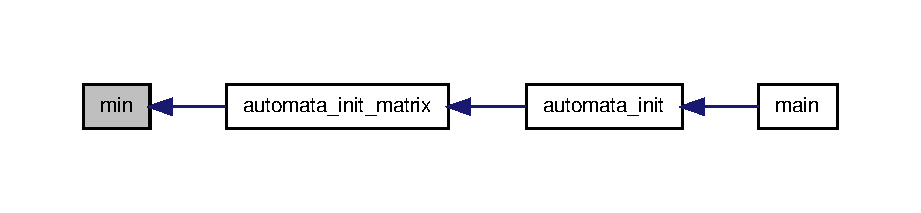
\includegraphics[width=350pt]{alr_8h_a52e321cf23b59535e518c501e8b7be56_icgraph}
\end{center}
\end{figure}


\hypertarget{alr_8h_a41b4a4554ba45c4eddf5c20f8f48f2b9}{\index{alr.\-h@{alr.\-h}!print\-\_\-atm@{print\-\_\-atm}}
\index{print\-\_\-atm@{print\-\_\-atm}!alr.h@{alr.\-h}}
\subsubsection[{print\-\_\-atm}]{\setlength{\rightskip}{0pt plus 5cm}void print\-\_\-atm (
\begin{DoxyParamCaption}
\item[{{\bf automata\-\_\-t} $\ast$}]{atm}
\end{DoxyParamCaption}
)}}\label{alr_8h_a41b4a4554ba45c4eddf5c20f8f48f2b9}


Printing the automata matrix. 


\begin{DoxyParams}{Parameters}
{\em atm,\-:} & Automata \\
\hline
\end{DoxyParams}


Definition at line 563 of file alr.\-c.



\subsection{Variable Documentation}
\hypertarget{alr_8h_a52eec20db404060f6d759e455219ac67}{\index{alr.\-h@{alr.\-h}!test\-\_\-run@{test\-\_\-run}}
\index{test\-\_\-run@{test\-\_\-run}!alr.h@{alr.\-h}}
\subsubsection[{test\-\_\-run}]{\setlength{\rightskip}{0pt plus 5cm}int test\-\_\-run}}\label{alr_8h_a52eec20db404060f6d759e455219ac67}


Definition at line 9 of file alr.\-h.


\hypertarget{main_8c}{\section{main.\-c File Reference}
\label{main_8c}\index{main.\-c@{main.\-c}}
}
{\ttfamily \#include $<$stdio.\-h$>$}\\*
{\ttfamily \#include $<$stdlib.\-h$>$}\\*
{\ttfamily \#include $<$time.\-h$>$}\\*
{\ttfamily \#include \char`\"{}types.\-h\char`\"{}}\\*
{\ttfamily \#include \char`\"{}matrix.\-h\char`\"{}}\\*
{\ttfamily \#include \char`\"{}alr.\-h\char`\"{}}\\*
{\ttfamily \#include \char`\"{}swarm.\-h\char`\"{}}\\*
Include dependency graph for main.\-c\-:\nopagebreak
\begin{figure}[H]
\begin{center}
\leavevmode
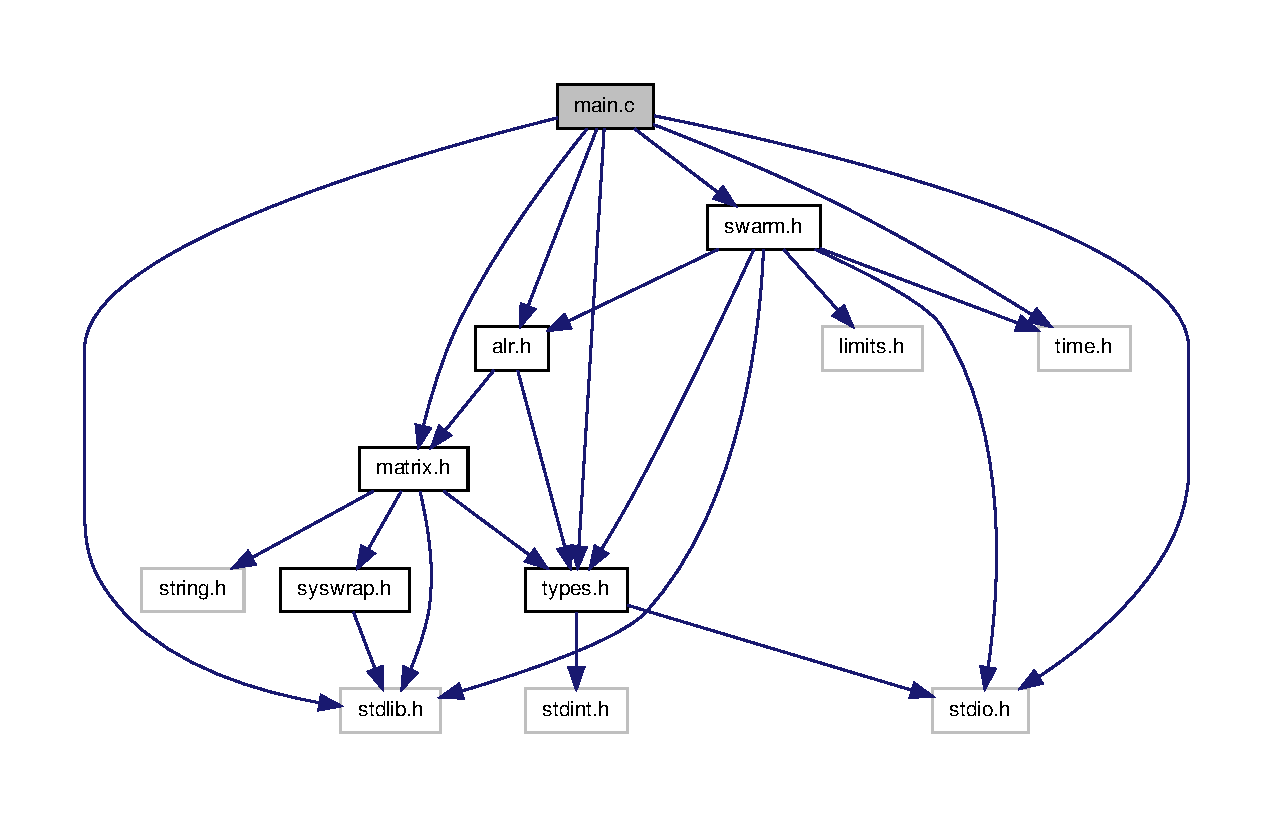
\includegraphics[width=350pt]{main_8c__incl}
\end{center}
\end{figure}
\subsection*{Functions}
\begin{DoxyCompactItemize}
\item 
int \hyperlink{main_8c_ac55bb64dc156887fc077ea35d9a4e483}{read\-\_\-data} (const char $\ast$filename, int $\ast$is\-\_\-rej, \hyperlink{types_8h_a4717ab46b712567c1482ad0f5b910027}{msize\-\_\-t} $\ast$splits\-\_\-num, \hyperlink{types_8h_a4717ab46b712567c1482ad0f5b910027}{msize\-\_\-t} $\ast$symbol\-\_\-class\-\_\-num, \hyperlink{types_8h_a594c3568b9a4bfb59d5d849a52dd9fe0}{fsize\-\_\-t} $\ast$feature\-\_\-num, \hyperlink{types_8h_a4717ab46b712567c1482ad0f5b910027}{msize\-\_\-t} $\ast$train\-\_\-size, \hyperlink{types_8h_a4717ab46b712567c1482ad0f5b910027}{msize\-\_\-t} $\ast$test\-\_\-size, double $\ast$max\-\_\-los, double $\ast$min\-\_\-los, double $\ast$nondet\-\_\-prop, \hyperlink{structfeature__t}{feature\-\_\-t} $\ast$$\ast$features, \hyperlink{structfeature__t}{feature\-\_\-t} $\ast$$\ast$test\-\_\-features, \hyperlink{structpso__params__t}{pso\-\_\-params\-\_\-t} $\ast$psopar, int $\ast$is\-\_\-read, \hyperlink{types_8h_a9052d9742e283c5c2169b5b06f8245f0}{feat\-\_\-t} $\ast$min\-\_\-tab, \hyperlink{types_8h_a9052d9742e283c5c2169b5b06f8245f0}{feat\-\_\-t} $\ast$max\-\_\-tab)
\begin{DoxyCompactList}\small\item\em Reads the data from input file (internal usage) \end{DoxyCompactList}\item 
int \hyperlink{main_8c_a3c04138a5bfe5d72780bb7e82a18e627}{main} (int argc, char $\ast$$\ast$argv)
\begin{DoxyCompactList}\small\item\em Entry point. \end{DoxyCompactList}\end{DoxyCompactItemize}


\subsection{Function Documentation}
\hypertarget{main_8c_a3c04138a5bfe5d72780bb7e82a18e627}{\index{main.\-c@{main.\-c}!main@{main}}
\index{main@{main}!main.c@{main.\-c}}
\subsubsection[{main}]{\setlength{\rightskip}{0pt plus 5cm}int main (
\begin{DoxyParamCaption}
\item[{int}]{argc, }
\item[{char $\ast$$\ast$}]{argv}
\end{DoxyParamCaption}
)}}\label{main_8c_a3c04138a5bfe5d72780bb7e82a18e627}


Entry point. 


\begin{DoxyParams}{Parameters}
{\em argc,\-:} & Number of arguments \\
\hline
{\em argv,\-:} & Argument list \\
\hline
\end{DoxyParams}
\begin{DoxyReturn}{Returns}

\end{DoxyReturn}


Definition at line 116 of file main.\-c.



Here is the call graph for this function\-:\nopagebreak
\begin{figure}[H]
\begin{center}
\leavevmode
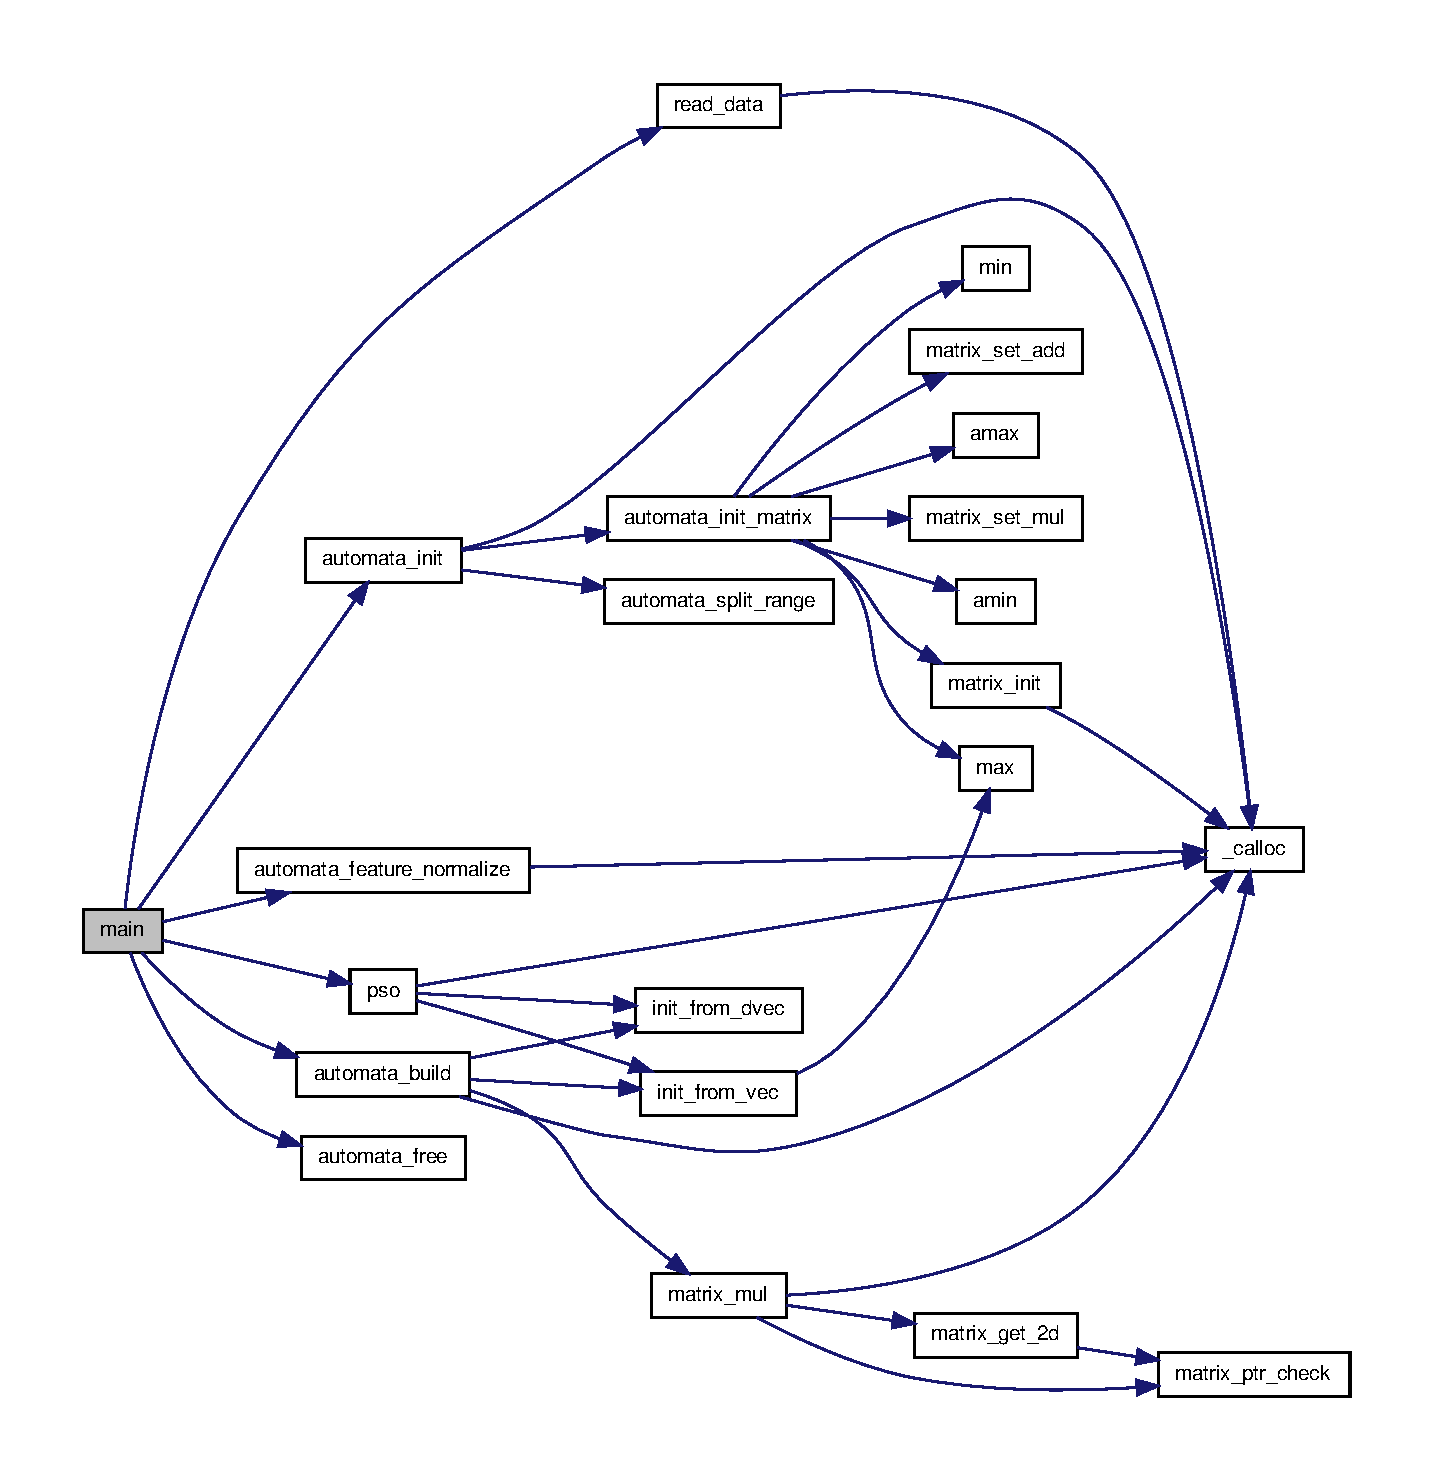
\includegraphics[width=350pt]{main_8c_a3c04138a5bfe5d72780bb7e82a18e627_cgraph}
\end{center}
\end{figure}


\hypertarget{main_8c_ac55bb64dc156887fc077ea35d9a4e483}{\index{main.\-c@{main.\-c}!read\-\_\-data@{read\-\_\-data}}
\index{read\-\_\-data@{read\-\_\-data}!main.c@{main.\-c}}
\subsubsection[{read\-\_\-data}]{\setlength{\rightskip}{0pt plus 5cm}int read\-\_\-data (
\begin{DoxyParamCaption}
\item[{const char $\ast$}]{filename, }
\item[{int $\ast$}]{is\-\_\-rej, }
\item[{{\bf msize\-\_\-t} $\ast$}]{splits\-\_\-num, }
\item[{{\bf msize\-\_\-t} $\ast$}]{symbol\-\_\-class\-\_\-num, }
\item[{{\bf fsize\-\_\-t} $\ast$}]{feature\-\_\-num, }
\item[{{\bf msize\-\_\-t} $\ast$}]{train\-\_\-size, }
\item[{{\bf msize\-\_\-t} $\ast$}]{test\-\_\-size, }
\item[{double $\ast$}]{max\-\_\-los, }
\item[{double $\ast$}]{min\-\_\-los, }
\item[{double $\ast$}]{nondet\-\_\-prop, }
\item[{{\bf feature\-\_\-t} $\ast$$\ast$}]{features, }
\item[{{\bf feature\-\_\-t} $\ast$$\ast$}]{test\-\_\-features, }
\item[{{\bf pso\-\_\-params\-\_\-t} $\ast$}]{psopar, }
\item[{int $\ast$}]{is\-\_\-read, }
\item[{{\bf feat\-\_\-t} $\ast$}]{min\-\_\-tab, }
\item[{{\bf feat\-\_\-t} $\ast$}]{max\-\_\-tab}
\end{DoxyParamCaption}
)}}\label{main_8c_ac55bb64dc156887fc077ea35d9a4e483}


Reads the data from input file (internal usage) 


\begin{DoxyParams}{Parameters}
{\em filename,\-:} & File name \\
\hline
{\em is\-\_\-rej,\-:} & Foreign symbols to recognize? \\
\hline
{\em splits\-\_\-num,\-:} & Number of splits of the \mbox{[}0..1\mbox{]} vector \\
\hline
{\em symbol\-\_\-class\-\_\-num,\-:} & Number of unique symbols \\
\hline
{\em feature\-\_\-num,\-:} & Number of features \\
\hline
{\em train\-\_\-size,\-:} & Number of symbols in training set \\
\hline
{\em test\-\_\-size,\-:} & Number of symbols in test set \\
\hline
{\em max\-\_\-los,\-:} & Max value of features (generated) \\
\hline
{\em min\-\_\-los,\-:} & Min value of features (generated) \\
\hline
{\em nondet\-\_\-prop,\-:} & Nondeterministic automata limit \\
\hline
{\em features,\-:} & Array of features of all symbols in training set \\
\hline
{\em test\-\_\-features,\-:} & Array of features ao all symbols in test set \\
\hline
{\em psopar,\-:} & P\-S\-O parameters \\
\hline
{\em is\-\_\-read,\-:} & Is data read from files? \\
\hline
{\em min\-\_\-tab,\-:} & Min values of features (read) \\
\hline
{\em max\-\_\-tab,\-:} & Max values of features (read) \\
\hline
\end{DoxyParams}
\begin{DoxyReturn}{Returns}

\end{DoxyReturn}


Definition at line 32 of file main.\-c.



Here is the call graph for this function\-:\nopagebreak
\begin{figure}[H]
\begin{center}
\leavevmode
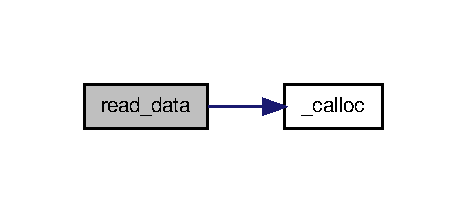
\includegraphics[width=224pt]{main_8c_ac55bb64dc156887fc077ea35d9a4e483_cgraph}
\end{center}
\end{figure}




Here is the caller graph for this function\-:\nopagebreak
\begin{figure}[H]
\begin{center}
\leavevmode
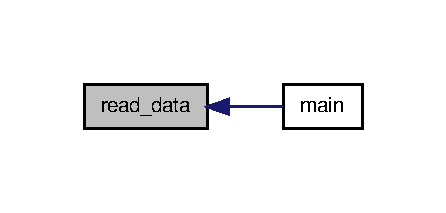
\includegraphics[width=214pt]{main_8c_ac55bb64dc156887fc077ea35d9a4e483_icgraph}
\end{center}
\end{figure}



\hypertarget{matrix_8c}{\section{matrix.\-c File Reference}
\label{matrix_8c}\index{matrix.\-c@{matrix.\-c}}
}
{\ttfamily \#include \char`\"{}matrix.\-h\char`\"{}}\\*
{\ttfamily \#include $<$assert.\-h$>$}\\*
Include dependency graph for matrix.\-c\-:\nopagebreak
\begin{figure}[H]
\begin{center}
\leavevmode
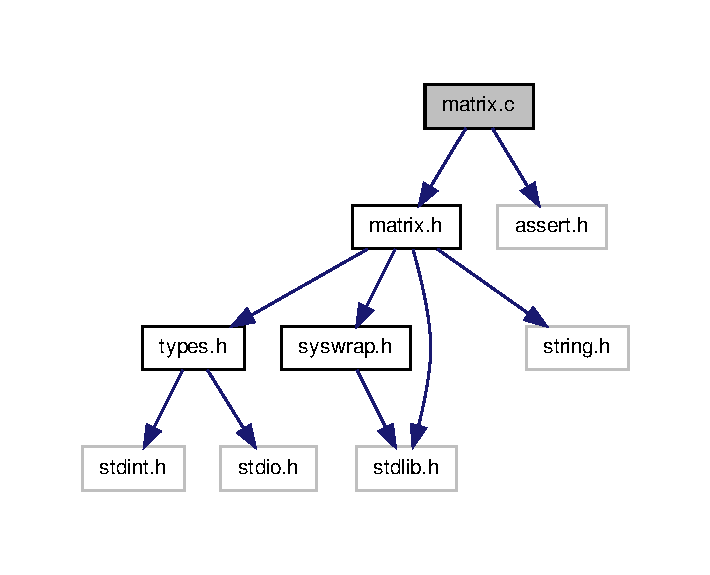
\includegraphics[width=341pt]{matrix_8c__incl}
\end{center}
\end{figure}
\subsection*{Functions}
\begin{DoxyCompactItemize}
\item 
\hyperlink{types_8h_a48f551883200abf3c18683f9a83a61a7}{mtx\-\_\-err\-\_\-code} \hyperlink{matrix_8c_aee9b7305c3eebba5ffa85cda39cd5de8}{matrix\-\_\-ptr\-\_\-check} (const \hyperlink{structmatrix__t}{matrix\-\_\-t} $\ast$mtx)
\begin{DoxyCompactList}\small\item\em initializes matrix with specified args \end{DoxyCompactList}\item 
\hyperlink{types_8h_a48f551883200abf3c18683f9a83a61a7}{mtx\-\_\-err\-\_\-code} \hyperlink{matrix_8c_a95d291945358f6ac92c9c98d69be87ff}{matrix\-\_\-init} (\hyperlink{structmatrix__t}{matrix\-\_\-t} $\ast$mtx, const \hyperlink{types_8h_a4717ab46b712567c1482ad0f5b910027}{msize\-\_\-t} m, const \hyperlink{types_8h_a4717ab46b712567c1482ad0f5b910027}{msize\-\_\-t} n, const \hyperlink{types_8h_a4717ab46b712567c1482ad0f5b910027}{msize\-\_\-t} k)
\begin{DoxyCompactList}\small\item\em initializes matrix with specified args \end{DoxyCompactList}\item 
\hyperlink{types_8h_a48f551883200abf3c18683f9a83a61a7}{mtx\-\_\-err\-\_\-code} \hyperlink{matrix_8c_a68ceaf153044028e938b7919cff70ebc}{matrix\-\_\-set\-\_\-cols} (\hyperlink{structmatrix__t}{matrix\-\_\-t} $\ast$mtx)
\begin{DoxyCompactList}\small\item\em randomly sets value one in every column of 2d array (get from split m) \end{DoxyCompactList}\item 
\hyperlink{types_8h_a48f551883200abf3c18683f9a83a61a7}{mtx\-\_\-err\-\_\-code} \hyperlink{matrix_8c_ae7c26cdd84bd1e5836eed766dc38a874}{matrix\-\_\-free} (\hyperlink{structmatrix__t}{matrix\-\_\-t} $\ast$mtx)
\begin{DoxyCompactList}\small\item\em frees and cleans memory in specified matrix \end{DoxyCompactList}\item 
\hyperlink{types_8h_a48f551883200abf3c18683f9a83a61a7}{mtx\-\_\-err\-\_\-code} \hyperlink{matrix_8c_a830977cb0de90bb59580e32cb18811a5}{matrix\-\_\-set\-\_\-add} (\hyperlink{structmatrix__t}{matrix\-\_\-t} $\ast$mtx, const \hyperlink{types_8h_a3472b426e98fe8245a0c3221c98d15a0}{mfunc\-\_\-add} add)
\begin{DoxyCompactList}\small\item\em sets a function responsible for add operation in matrix multiplication \end{DoxyCompactList}\item 
\hyperlink{types_8h_a48f551883200abf3c18683f9a83a61a7}{mtx\-\_\-err\-\_\-code} \hyperlink{matrix_8c_acfbad898e332491b196de01a9ee4fa66}{matrix\-\_\-set\-\_\-mul} (\hyperlink{structmatrix__t}{matrix\-\_\-t} $\ast$mtx, const \hyperlink{types_8h_a8552194635c37d32de855f3b57657efa}{mfunc\-\_\-mul} mul)
\begin{DoxyCompactList}\small\item\em sets a function responsible for mul operation in matrix multiplication \end{DoxyCompactList}\item 
\hyperlink{types_8h_a48f551883200abf3c18683f9a83a61a7}{mtx\-\_\-err\-\_\-code} \hyperlink{matrix_8c_afa9f2f9d937965ae876c3a641a2f0b86}{matrix\-\_\-mul} (const \hyperlink{structmatrix__t}{matrix\-\_\-t} $\ast$mtx, const \hyperlink{types_8h_a4717ab46b712567c1482ad0f5b910027}{msize\-\_\-t} m, const \hyperlink{types_8h_a170cb8b681dd48ced181eb10f1c5c7c8}{mvec1\-\_\-t} vec1, const \hyperlink{types_8h_a4717ab46b712567c1482ad0f5b910027}{msize\-\_\-t} vec\-\_\-size, \hyperlink{types_8h_a18fafbc4cdb252f40f312814635aa706}{mvec2\-\_\-t} $\ast$vec2)
\begin{DoxyCompactList}\small\item\em matrix x vector multiplication function \end{DoxyCompactList}\item 
\hyperlink{types_8h_a48f551883200abf3c18683f9a83a61a7}{mtx\-\_\-err\-\_\-code} \hyperlink{matrix_8c_aef4c14420a092739627e2468af43e1d1}{matrix\-\_\-get\-\_\-2d} (const \hyperlink{structmatrix__t}{matrix\-\_\-t} $\ast$mtx, const \hyperlink{types_8h_a4717ab46b712567c1482ad0f5b910027}{msize\-\_\-t} m, \hyperlink{types_8h_a18fafbc4cdb252f40f312814635aa706}{mvec2\-\_\-t} $\ast$vec2)
\begin{DoxyCompactList}\small\item\em gets a 2d matrix from 3d matrix using specified split value \end{DoxyCompactList}\item 
\hyperlink{types_8h_a48f551883200abf3c18683f9a83a61a7}{mtx\-\_\-err\-\_\-code} \hyperlink{matrix_8c_a82363b691c68807628aa231b1a90308c}{matrix\-\_\-set\-\_\-val} (\hyperlink{structmatrix__t}{matrix\-\_\-t} $\ast$mtx, const \hyperlink{types_8h_a4717ab46b712567c1482ad0f5b910027}{msize\-\_\-t} m, const \hyperlink{types_8h_a4717ab46b712567c1482ad0f5b910027}{msize\-\_\-t} n, const \hyperlink{types_8h_a4717ab46b712567c1482ad0f5b910027}{msize\-\_\-t} k, const \hyperlink{types_8h_a7bc9d9790537ce02dc19f7fc4080b98b}{melem\-\_\-t} val)
\begin{DoxyCompactList}\small\item\em sets a value on specified position \end{DoxyCompactList}\item 
\hyperlink{types_8h_a48f551883200abf3c18683f9a83a61a7}{mtx\-\_\-err\-\_\-code} \hyperlink{matrix_8c_a6118c1cdc8b1b3c4abd5f6bd83fc5a8e}{matrix\-\_\-show} (const \hyperlink{structmatrix__t}{matrix\-\_\-t} $\ast$mtx, const \hyperlink{types_8h_a4717ab46b712567c1482ad0f5b910027}{msize\-\_\-t} m)
\begin{DoxyCompactList}\small\item\em shows matrix in human readable format \end{DoxyCompactList}\end{DoxyCompactItemize}


\subsection{Function Documentation}
\hypertarget{matrix_8c_ae7c26cdd84bd1e5836eed766dc38a874}{\index{matrix.\-c@{matrix.\-c}!matrix\-\_\-free@{matrix\-\_\-free}}
\index{matrix\-\_\-free@{matrix\-\_\-free}!matrix.c@{matrix.\-c}}
\subsubsection[{matrix\-\_\-free}]{\setlength{\rightskip}{0pt plus 5cm}{\bf mtx\-\_\-err\-\_\-code} matrix\-\_\-free (
\begin{DoxyParamCaption}
\item[{{\bf matrix\-\_\-t} $\ast$}]{mtx}
\end{DoxyParamCaption}
)}}\label{matrix_8c_ae7c26cdd84bd1e5836eed766dc38a874}


frees and cleans memory in specified matrix 


\begin{DoxyParams}{Parameters}
{\em mtx} & pointer to \hyperlink{structmatrix__t}{matrix\-\_\-t} structure\\
\hline
\end{DoxyParams}
\begin{DoxyReturn}{Returns}
M\-T\-X\-\_\-\-O\-K if function succeed, error code in other cases 
\end{DoxyReturn}


Definition at line 68 of file matrix.\-c.



Here is the call graph for this function\-:\nopagebreak
\begin{figure}[H]
\begin{center}
\leavevmode
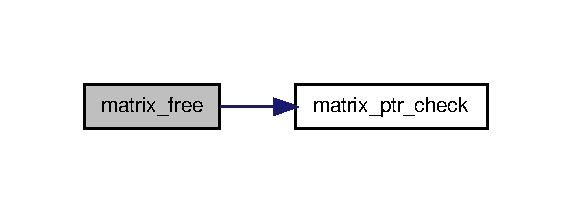
\includegraphics[width=274pt]{matrix_8c_ae7c26cdd84bd1e5836eed766dc38a874_cgraph}
\end{center}
\end{figure}




Here is the caller graph for this function\-:\nopagebreak
\begin{figure}[H]
\begin{center}
\leavevmode
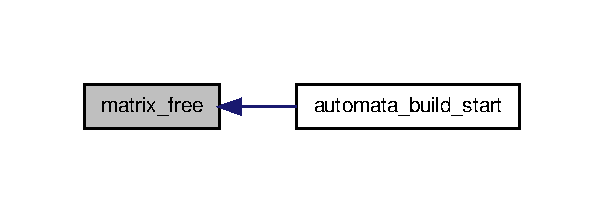
\includegraphics[width=290pt]{matrix_8c_ae7c26cdd84bd1e5836eed766dc38a874_icgraph}
\end{center}
\end{figure}


\hypertarget{matrix_8c_aef4c14420a092739627e2468af43e1d1}{\index{matrix.\-c@{matrix.\-c}!matrix\-\_\-get\-\_\-2d@{matrix\-\_\-get\-\_\-2d}}
\index{matrix\-\_\-get\-\_\-2d@{matrix\-\_\-get\-\_\-2d}!matrix.c@{matrix.\-c}}
\subsubsection[{matrix\-\_\-get\-\_\-2d}]{\setlength{\rightskip}{0pt plus 5cm}{\bf mtx\-\_\-err\-\_\-code} matrix\-\_\-get\-\_\-2d (
\begin{DoxyParamCaption}
\item[{const {\bf matrix\-\_\-t} $\ast$}]{mtx, }
\item[{const {\bf msize\-\_\-t}}]{m, }
\item[{{\bf mvec2\-\_\-t} $\ast$}]{vec2}
\end{DoxyParamCaption}
)}}\label{matrix_8c_aef4c14420a092739627e2468af43e1d1}


gets a 2d matrix from 3d matrix using specified split value 


\begin{DoxyParams}{Parameters}
{\em mtx} & pointer to \hyperlink{structmatrix__t}{matrix\-\_\-t} structure \\
\hline
{\em m} & split value \\
\hline
{\em vec2(out)} & pointer to mvec2\-\_\-t, that will point to 2d matrix\\
\hline
\end{DoxyParams}
\begin{DoxyReturn}{Returns}
M\-T\-X\-\_\-\-O\-K if function succeed, error code in other cases 
\end{DoxyReturn}


Definition at line 155 of file matrix.\-c.



Here is the call graph for this function\-:\nopagebreak
\begin{figure}[H]
\begin{center}
\leavevmode
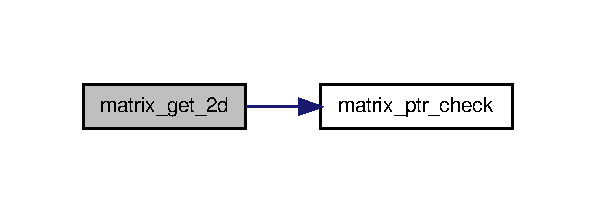
\includegraphics[width=286pt]{matrix_8c_aef4c14420a092739627e2468af43e1d1_cgraph}
\end{center}
\end{figure}




Here is the caller graph for this function\-:\nopagebreak
\begin{figure}[H]
\begin{center}
\leavevmode
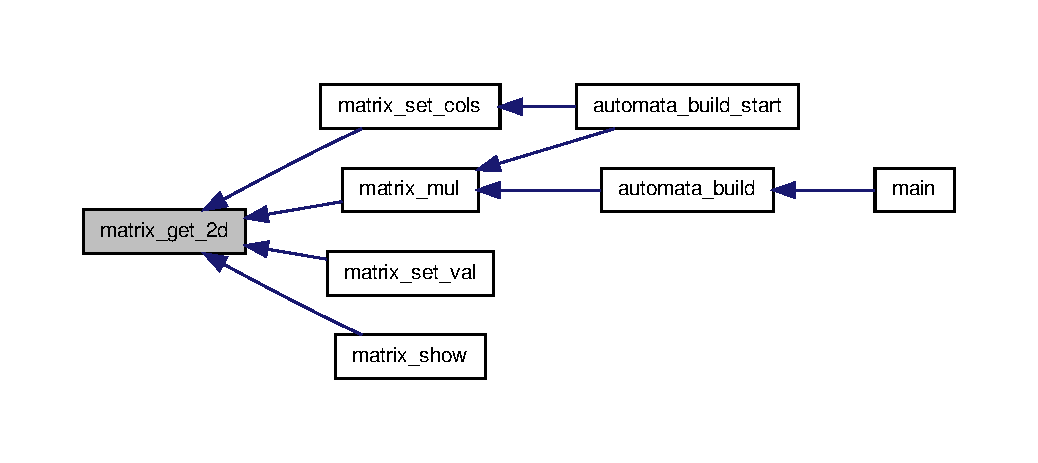
\includegraphics[width=350pt]{matrix_8c_aef4c14420a092739627e2468af43e1d1_icgraph}
\end{center}
\end{figure}


\hypertarget{matrix_8c_a95d291945358f6ac92c9c98d69be87ff}{\index{matrix.\-c@{matrix.\-c}!matrix\-\_\-init@{matrix\-\_\-init}}
\index{matrix\-\_\-init@{matrix\-\_\-init}!matrix.c@{matrix.\-c}}
\subsubsection[{matrix\-\_\-init}]{\setlength{\rightskip}{0pt plus 5cm}{\bf mtx\-\_\-err\-\_\-code} matrix\-\_\-init (
\begin{DoxyParamCaption}
\item[{{\bf matrix\-\_\-t} $\ast$}]{mtx, }
\item[{const {\bf msize\-\_\-t}}]{m, }
\item[{const {\bf msize\-\_\-t}}]{n, }
\item[{const {\bf msize\-\_\-t}}]{k}
\end{DoxyParamCaption}
)}}\label{matrix_8c_a95d291945358f6ac92c9c98d69be87ff}


initializes matrix with specified args 


\begin{DoxyParams}{Parameters}
{\em mtx} & pointer to \hyperlink{structmatrix__t}{matrix\-\_\-t} structure \\
\hline
{\em m} & third dimension \\
\hline
{\em n} & second dimension \\
\hline
{\em k} & first dimension\\
\hline
\end{DoxyParams}
\begin{DoxyReturn}{Returns}
M\-T\-X\-\_\-\-O\-K if function succeed, error code in other cases 
\end{DoxyReturn}


Definition at line 15 of file matrix.\-c.



Here is the call graph for this function\-:\nopagebreak
\begin{figure}[H]
\begin{center}
\leavevmode
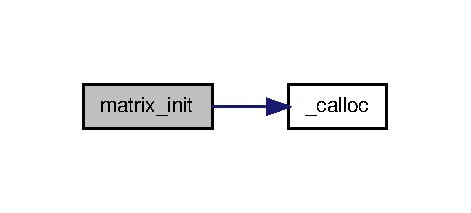
\includegraphics[width=226pt]{matrix_8c_a95d291945358f6ac92c9c98d69be87ff_cgraph}
\end{center}
\end{figure}




Here is the caller graph for this function\-:\nopagebreak
\begin{figure}[H]
\begin{center}
\leavevmode
\includegraphics[width=350pt]{matrix_8c_a95d291945358f6ac92c9c98d69be87ff_icgraph}
\end{center}
\end{figure}


\hypertarget{matrix_8c_afa9f2f9d937965ae876c3a641a2f0b86}{\index{matrix.\-c@{matrix.\-c}!matrix\-\_\-mul@{matrix\-\_\-mul}}
\index{matrix\-\_\-mul@{matrix\-\_\-mul}!matrix.c@{matrix.\-c}}
\subsubsection[{matrix\-\_\-mul}]{\setlength{\rightskip}{0pt plus 5cm}{\bf mtx\-\_\-err\-\_\-code} matrix\-\_\-mul (
\begin{DoxyParamCaption}
\item[{const {\bf matrix\-\_\-t} $\ast$}]{mtx, }
\item[{const {\bf msize\-\_\-t}}]{m, }
\item[{const {\bf mvec1\-\_\-t}}]{vec1, }
\item[{const {\bf msize\-\_\-t}}]{vec\-\_\-size, }
\item[{{\bf mvec2\-\_\-t} $\ast$}]{vec2}
\end{DoxyParamCaption}
)}}\label{matrix_8c_afa9f2f9d937965ae876c3a641a2f0b86}


matrix x vector multiplication function 


\begin{DoxyParams}{Parameters}
{\em mtx} & pointer to \hyperlink{structmatrix__t}{matrix\-\_\-t} structure \\
\hline
{\em m} & split value \\
\hline
{\em vec1} & vector \\
\hline
{\em vec\-\_\-size} & lenght of vector \\
\hline
{\em vec2(out)} & pointer to mvec2\-\_\-t filled with output multiplication vector values (!!!\-S\-H\-O\-U\-L\-D B\-E F\-R\-E\-E\-D!!!)\\
\hline
\end{DoxyParams}
\begin{DoxyReturn}{Returns}
M\-T\-X\-\_\-\-O\-K if function succeed, error code in other cases 
\end{DoxyReturn}


Definition at line 118 of file matrix.\-c.



Here is the call graph for this function\-:\nopagebreak
\begin{figure}[H]
\begin{center}
\leavevmode
\includegraphics[width=350pt]{matrix_8c_afa9f2f9d937965ae876c3a641a2f0b86_cgraph}
\end{center}
\end{figure}




Here is the caller graph for this function\-:\nopagebreak
\begin{figure}[H]
\begin{center}
\leavevmode
\includegraphics[width=350pt]{matrix_8c_afa9f2f9d937965ae876c3a641a2f0b86_icgraph}
\end{center}
\end{figure}


\hypertarget{matrix_8c_aee9b7305c3eebba5ffa85cda39cd5de8}{\index{matrix.\-c@{matrix.\-c}!matrix\-\_\-ptr\-\_\-check@{matrix\-\_\-ptr\-\_\-check}}
\index{matrix\-\_\-ptr\-\_\-check@{matrix\-\_\-ptr\-\_\-check}!matrix.c@{matrix.\-c}}
\subsubsection[{matrix\-\_\-ptr\-\_\-check}]{\setlength{\rightskip}{0pt plus 5cm}{\bf mtx\-\_\-err\-\_\-code} matrix\-\_\-ptr\-\_\-check (
\begin{DoxyParamCaption}
\item[{const {\bf matrix\-\_\-t} $\ast$}]{mtx}
\end{DoxyParamCaption}
)}}\label{matrix_8c_aee9b7305c3eebba5ffa85cda39cd5de8}


initializes matrix with specified args 

2d/3d matrix functions 
\begin{DoxyParams}{Parameters}
{\em mtx} & pointer to \hyperlink{structmatrix__t}{matrix\-\_\-t} structure \\
\hline
{\em m} & third dimension \\
\hline
{\em n} & second dimension \\
\hline
{\em k} & first dimension\\
\hline
\end{DoxyParams}
\begin{DoxyReturn}{Returns}
M\-T\-X\-\_\-\-O\-K if function succeed, error code in other cases 
\end{DoxyReturn}


Definition at line 5 of file matrix.\-c.



Here is the caller graph for this function\-:\nopagebreak
\begin{figure}[H]
\begin{center}
\leavevmode
\includegraphics[width=350pt]{matrix_8c_aee9b7305c3eebba5ffa85cda39cd5de8_icgraph}
\end{center}
\end{figure}


\hypertarget{matrix_8c_a830977cb0de90bb59580e32cb18811a5}{\index{matrix.\-c@{matrix.\-c}!matrix\-\_\-set\-\_\-add@{matrix\-\_\-set\-\_\-add}}
\index{matrix\-\_\-set\-\_\-add@{matrix\-\_\-set\-\_\-add}!matrix.c@{matrix.\-c}}
\subsubsection[{matrix\-\_\-set\-\_\-add}]{\setlength{\rightskip}{0pt plus 5cm}{\bf mtx\-\_\-err\-\_\-code} matrix\-\_\-set\-\_\-add (
\begin{DoxyParamCaption}
\item[{{\bf matrix\-\_\-t} $\ast$}]{mtx, }
\item[{const {\bf mfunc\-\_\-add}}]{add}
\end{DoxyParamCaption}
)}}\label{matrix_8c_a830977cb0de90bb59580e32cb18811a5}


sets a function responsible for add operation in matrix multiplication 


\begin{DoxyParams}{Parameters}
{\em mtx} & pointer to \hyperlink{structmatrix__t}{matrix\-\_\-t} structure \\
\hline
{\em add} & pointer to add operation function\\
\hline
\end{DoxyParams}
\begin{DoxyReturn}{Returns}
M\-T\-X\-\_\-\-O\-K if function succeed, error code in other cases 
\end{DoxyReturn}


Definition at line 98 of file matrix.\-c.



Here is the caller graph for this function\-:\nopagebreak
\begin{figure}[H]
\begin{center}
\leavevmode
\includegraphics[width=350pt]{matrix_8c_a830977cb0de90bb59580e32cb18811a5_icgraph}
\end{center}
\end{figure}


\hypertarget{matrix_8c_a68ceaf153044028e938b7919cff70ebc}{\index{matrix.\-c@{matrix.\-c}!matrix\-\_\-set\-\_\-cols@{matrix\-\_\-set\-\_\-cols}}
\index{matrix\-\_\-set\-\_\-cols@{matrix\-\_\-set\-\_\-cols}!matrix.c@{matrix.\-c}}
\subsubsection[{matrix\-\_\-set\-\_\-cols}]{\setlength{\rightskip}{0pt plus 5cm}{\bf mtx\-\_\-err\-\_\-code} matrix\-\_\-set\-\_\-cols (
\begin{DoxyParamCaption}
\item[{{\bf matrix\-\_\-t} $\ast$}]{mtx}
\end{DoxyParamCaption}
)}}\label{matrix_8c_a68ceaf153044028e938b7919cff70ebc}


randomly sets value one in every column of 2d array (get from split m) 


\begin{DoxyParams}{Parameters}
{\em mtx} & pointer to \hyperlink{structmatrix__t}{matrix\-\_\-t} structure\\
\hline
\end{DoxyParams}
\begin{DoxyReturn}{Returns}
M\-T\-X\-\_\-\-O\-K if function succeed, error code in other cases 
\end{DoxyReturn}


Definition at line 49 of file matrix.\-c.



Here is the call graph for this function\-:\nopagebreak
\begin{figure}[H]
\begin{center}
\leavevmode
\includegraphics[width=350pt]{matrix_8c_a68ceaf153044028e938b7919cff70ebc_cgraph}
\end{center}
\end{figure}




Here is the caller graph for this function\-:\nopagebreak
\begin{figure}[H]
\begin{center}
\leavevmode
\includegraphics[width=310pt]{matrix_8c_a68ceaf153044028e938b7919cff70ebc_icgraph}
\end{center}
\end{figure}


\hypertarget{matrix_8c_acfbad898e332491b196de01a9ee4fa66}{\index{matrix.\-c@{matrix.\-c}!matrix\-\_\-set\-\_\-mul@{matrix\-\_\-set\-\_\-mul}}
\index{matrix\-\_\-set\-\_\-mul@{matrix\-\_\-set\-\_\-mul}!matrix.c@{matrix.\-c}}
\subsubsection[{matrix\-\_\-set\-\_\-mul}]{\setlength{\rightskip}{0pt plus 5cm}{\bf mtx\-\_\-err\-\_\-code} matrix\-\_\-set\-\_\-mul (
\begin{DoxyParamCaption}
\item[{{\bf matrix\-\_\-t} $\ast$}]{mtx, }
\item[{const {\bf mfunc\-\_\-mul}}]{mul}
\end{DoxyParamCaption}
)}}\label{matrix_8c_acfbad898e332491b196de01a9ee4fa66}


sets a function responsible for mul operation in matrix multiplication 


\begin{DoxyParams}{Parameters}
{\em mtx} & pointer to \hyperlink{structmatrix__t}{matrix\-\_\-t} structure \\
\hline
{\em mul} & pointer to mul operation function\\
\hline
\end{DoxyParams}
\begin{DoxyReturn}{Returns}
M\-T\-X\-\_\-\-O\-K if function succeed, error code in other cases 
\end{DoxyReturn}


Definition at line 108 of file matrix.\-c.



Here is the caller graph for this function\-:\nopagebreak
\begin{figure}[H]
\begin{center}
\leavevmode
\includegraphics[width=350pt]{matrix_8c_acfbad898e332491b196de01a9ee4fa66_icgraph}
\end{center}
\end{figure}


\hypertarget{matrix_8c_a82363b691c68807628aa231b1a90308c}{\index{matrix.\-c@{matrix.\-c}!matrix\-\_\-set\-\_\-val@{matrix\-\_\-set\-\_\-val}}
\index{matrix\-\_\-set\-\_\-val@{matrix\-\_\-set\-\_\-val}!matrix.c@{matrix.\-c}}
\subsubsection[{matrix\-\_\-set\-\_\-val}]{\setlength{\rightskip}{0pt plus 5cm}{\bf mtx\-\_\-err\-\_\-code} matrix\-\_\-set\-\_\-val (
\begin{DoxyParamCaption}
\item[{{\bf matrix\-\_\-t} $\ast$}]{mtx, }
\item[{const {\bf msize\-\_\-t}}]{m, }
\item[{const {\bf msize\-\_\-t}}]{n, }
\item[{const {\bf msize\-\_\-t}}]{k, }
\item[{const {\bf melem\-\_\-t}}]{val}
\end{DoxyParamCaption}
)}}\label{matrix_8c_a82363b691c68807628aa231b1a90308c}


sets a value on specified position 


\begin{DoxyParams}{Parameters}
{\em mtx} & pointer to \hyperlink{structmatrix__t}{matrix\-\_\-t} structure \\
\hline
{\em m} & split value \\
\hline
{\em n} & second dimension \\
\hline
{\em k} & first dimension \\
\hline
{\em val} & value to set\\
\hline
\end{DoxyParams}
\begin{DoxyReturn}{Returns}
M\-T\-X\-\_\-\-O\-K if function succeed, error code in other cases 
\end{DoxyReturn}


Definition at line 173 of file matrix.\-c.



Here is the call graph for this function\-:\nopagebreak
\begin{figure}[H]
\begin{center}
\leavevmode
\includegraphics[width=350pt]{matrix_8c_a82363b691c68807628aa231b1a90308c_cgraph}
\end{center}
\end{figure}


\hypertarget{matrix_8c_a6118c1cdc8b1b3c4abd5f6bd83fc5a8e}{\index{matrix.\-c@{matrix.\-c}!matrix\-\_\-show@{matrix\-\_\-show}}
\index{matrix\-\_\-show@{matrix\-\_\-show}!matrix.c@{matrix.\-c}}
\subsubsection[{matrix\-\_\-show}]{\setlength{\rightskip}{0pt plus 5cm}{\bf mtx\-\_\-err\-\_\-code} matrix\-\_\-show (
\begin{DoxyParamCaption}
\item[{const {\bf matrix\-\_\-t} $\ast$}]{mtx, }
\item[{const {\bf msize\-\_\-t}}]{m}
\end{DoxyParamCaption}
)}}\label{matrix_8c_a6118c1cdc8b1b3c4abd5f6bd83fc5a8e}


shows matrix in human readable format 


\begin{DoxyParams}{Parameters}
{\em mtx} & pointer to \hyperlink{structmatrix__t}{matrix\-\_\-t} structure \\
\hline
{\em m} & split value\\
\hline
\end{DoxyParams}
\begin{DoxyReturn}{Returns}
M\-T\-X\-\_\-\-O\-K if function succeed, error code in other cases 
\end{DoxyReturn}


Definition at line 189 of file matrix.\-c.



Here is the call graph for this function\-:\nopagebreak
\begin{figure}[H]
\begin{center}
\leavevmode
\includegraphics[width=350pt]{matrix_8c_a6118c1cdc8b1b3c4abd5f6bd83fc5a8e_cgraph}
\end{center}
\end{figure}



\hypertarget{matrix_8h}{\section{matrix.\-h File Reference}
\label{matrix_8h}\index{matrix.\-h@{matrix.\-h}}
}
{\ttfamily \#include \char`\"{}types.\-h\char`\"{}}\\*
{\ttfamily \#include \char`\"{}syswrap.\-h\char`\"{}}\\*
{\ttfamily \#include $<$stdlib.\-h$>$}\\*
{\ttfamily \#include $<$string.\-h$>$}\\*
Include dependency graph for matrix.\-h\-:\nopagebreak
\begin{figure}[H]
\begin{center}
\leavevmode
\includegraphics[width=341pt]{matrix_8h__incl}
\end{center}
\end{figure}
This graph shows which files directly or indirectly include this file\-:\nopagebreak
\begin{figure}[H]
\begin{center}
\leavevmode
\includegraphics[width=330pt]{matrix_8h__dep__incl}
\end{center}
\end{figure}
\subsection*{Data Structures}
\begin{DoxyCompactItemize}
\item 
struct \hyperlink{structmatrix__t}{matrix\-\_\-t}
\begin{DoxyCompactList}\small\item\em 3d matrix structure m \-:= split n, k \-:= states add \-:= add operator handler mul \-:= mul operator handler \end{DoxyCompactList}\end{DoxyCompactItemize}
\subsection*{Functions}
\begin{DoxyCompactItemize}
\item 
\hyperlink{types_8h_a48f551883200abf3c18683f9a83a61a7}{mtx\-\_\-err\-\_\-code} \hyperlink{matrix_8h_aee9b7305c3eebba5ffa85cda39cd5de8}{matrix\-\_\-ptr\-\_\-check} (const \hyperlink{structmatrix__t}{matrix\-\_\-t} $\ast$mtx)
\begin{DoxyCompactList}\small\item\em initializes matrix with specified args \end{DoxyCompactList}\item 
\hyperlink{types_8h_a48f551883200abf3c18683f9a83a61a7}{mtx\-\_\-err\-\_\-code} \hyperlink{matrix_8h_a95d291945358f6ac92c9c98d69be87ff}{matrix\-\_\-init} (\hyperlink{structmatrix__t}{matrix\-\_\-t} $\ast$mtx, const \hyperlink{types_8h_a4717ab46b712567c1482ad0f5b910027}{msize\-\_\-t} m, const \hyperlink{types_8h_a4717ab46b712567c1482ad0f5b910027}{msize\-\_\-t} n, const \hyperlink{types_8h_a4717ab46b712567c1482ad0f5b910027}{msize\-\_\-t} k)
\begin{DoxyCompactList}\small\item\em initializes matrix with specified args \end{DoxyCompactList}\item 
\hyperlink{types_8h_a48f551883200abf3c18683f9a83a61a7}{mtx\-\_\-err\-\_\-code} \hyperlink{matrix_8h_a68ceaf153044028e938b7919cff70ebc}{matrix\-\_\-set\-\_\-cols} (\hyperlink{structmatrix__t}{matrix\-\_\-t} $\ast$mtx)
\begin{DoxyCompactList}\small\item\em randomly sets value one in every column of 2d array (get from split m) \end{DoxyCompactList}\item 
\hyperlink{types_8h_a48f551883200abf3c18683f9a83a61a7}{mtx\-\_\-err\-\_\-code} \hyperlink{matrix_8h_ae7c26cdd84bd1e5836eed766dc38a874}{matrix\-\_\-free} (\hyperlink{structmatrix__t}{matrix\-\_\-t} $\ast$mtx)
\begin{DoxyCompactList}\small\item\em frees and cleans memory in specified matrix \end{DoxyCompactList}\item 
\hyperlink{types_8h_a48f551883200abf3c18683f9a83a61a7}{mtx\-\_\-err\-\_\-code} \hyperlink{matrix_8h_a830977cb0de90bb59580e32cb18811a5}{matrix\-\_\-set\-\_\-add} (\hyperlink{structmatrix__t}{matrix\-\_\-t} $\ast$mtx, const \hyperlink{types_8h_a3472b426e98fe8245a0c3221c98d15a0}{mfunc\-\_\-add} add)
\begin{DoxyCompactList}\small\item\em sets a function responsible for add operation in matrix multiplication \end{DoxyCompactList}\item 
\hyperlink{types_8h_a48f551883200abf3c18683f9a83a61a7}{mtx\-\_\-err\-\_\-code} \hyperlink{matrix_8h_acfbad898e332491b196de01a9ee4fa66}{matrix\-\_\-set\-\_\-mul} (\hyperlink{structmatrix__t}{matrix\-\_\-t} $\ast$mtx, const \hyperlink{types_8h_a8552194635c37d32de855f3b57657efa}{mfunc\-\_\-mul} mul)
\begin{DoxyCompactList}\small\item\em sets a function responsible for mul operation in matrix multiplication \end{DoxyCompactList}\item 
\hyperlink{types_8h_a48f551883200abf3c18683f9a83a61a7}{mtx\-\_\-err\-\_\-code} \hyperlink{matrix_8h_afa9f2f9d937965ae876c3a641a2f0b86}{matrix\-\_\-mul} (const \hyperlink{structmatrix__t}{matrix\-\_\-t} $\ast$mtx, const \hyperlink{types_8h_a4717ab46b712567c1482ad0f5b910027}{msize\-\_\-t} m, const \hyperlink{types_8h_a170cb8b681dd48ced181eb10f1c5c7c8}{mvec1\-\_\-t} vec1, const \hyperlink{types_8h_a4717ab46b712567c1482ad0f5b910027}{msize\-\_\-t} vec\-\_\-size, \hyperlink{types_8h_a18fafbc4cdb252f40f312814635aa706}{mvec2\-\_\-t} $\ast$vec2)
\begin{DoxyCompactList}\small\item\em matrix x vector multiplication function \end{DoxyCompactList}\item 
\hyperlink{types_8h_a48f551883200abf3c18683f9a83a61a7}{mtx\-\_\-err\-\_\-code} \hyperlink{matrix_8h_aef4c14420a092739627e2468af43e1d1}{matrix\-\_\-get\-\_\-2d} (const \hyperlink{structmatrix__t}{matrix\-\_\-t} $\ast$mtx, const \hyperlink{types_8h_a4717ab46b712567c1482ad0f5b910027}{msize\-\_\-t} m, \hyperlink{types_8h_a18fafbc4cdb252f40f312814635aa706}{mvec2\-\_\-t} $\ast$vec2)
\begin{DoxyCompactList}\small\item\em gets a 2d matrix from 3d matrix using specified split value \end{DoxyCompactList}\item 
\hyperlink{types_8h_a48f551883200abf3c18683f9a83a61a7}{mtx\-\_\-err\-\_\-code} \hyperlink{matrix_8h_a82363b691c68807628aa231b1a90308c}{matrix\-\_\-set\-\_\-val} (\hyperlink{structmatrix__t}{matrix\-\_\-t} $\ast$mtx, const \hyperlink{types_8h_a4717ab46b712567c1482ad0f5b910027}{msize\-\_\-t} m, const \hyperlink{types_8h_a4717ab46b712567c1482ad0f5b910027}{msize\-\_\-t} n, const \hyperlink{types_8h_a4717ab46b712567c1482ad0f5b910027}{msize\-\_\-t} k, const \hyperlink{types_8h_a7bc9d9790537ce02dc19f7fc4080b98b}{melem\-\_\-t} val)
\begin{DoxyCompactList}\small\item\em sets a value on specified position \end{DoxyCompactList}\item 
\hyperlink{types_8h_a48f551883200abf3c18683f9a83a61a7}{mtx\-\_\-err\-\_\-code} \hyperlink{matrix_8h_a6118c1cdc8b1b3c4abd5f6bd83fc5a8e}{matrix\-\_\-show} (const \hyperlink{structmatrix__t}{matrix\-\_\-t} $\ast$mtx, const \hyperlink{types_8h_a4717ab46b712567c1482ad0f5b910027}{msize\-\_\-t} m)
\begin{DoxyCompactList}\small\item\em shows matrix in human readable format \end{DoxyCompactList}\end{DoxyCompactItemize}


\subsection{Function Documentation}
\hypertarget{matrix_8h_ae7c26cdd84bd1e5836eed766dc38a874}{\index{matrix.\-h@{matrix.\-h}!matrix\-\_\-free@{matrix\-\_\-free}}
\index{matrix\-\_\-free@{matrix\-\_\-free}!matrix.h@{matrix.\-h}}
\subsubsection[{matrix\-\_\-free}]{\setlength{\rightskip}{0pt plus 5cm}{\bf mtx\-\_\-err\-\_\-code} matrix\-\_\-free (
\begin{DoxyParamCaption}
\item[{{\bf matrix\-\_\-t} $\ast$}]{mtx}
\end{DoxyParamCaption}
)}}\label{matrix_8h_ae7c26cdd84bd1e5836eed766dc38a874}


frees and cleans memory in specified matrix 


\begin{DoxyParams}{Parameters}
{\em mtx} & pointer to \hyperlink{structmatrix__t}{matrix\-\_\-t} structure\\
\hline
\end{DoxyParams}
\begin{DoxyReturn}{Returns}
M\-T\-X\-\_\-\-O\-K if function succeed, error code in other cases 
\end{DoxyReturn}


Definition at line 68 of file matrix.\-c.



Here is the call graph for this function\-:\nopagebreak
\begin{figure}[H]
\begin{center}
\leavevmode
\includegraphics[width=274pt]{matrix_8h_ae7c26cdd84bd1e5836eed766dc38a874_cgraph}
\end{center}
\end{figure}




Here is the caller graph for this function\-:\nopagebreak
\begin{figure}[H]
\begin{center}
\leavevmode
\includegraphics[width=290pt]{matrix_8h_ae7c26cdd84bd1e5836eed766dc38a874_icgraph}
\end{center}
\end{figure}


\hypertarget{matrix_8h_aef4c14420a092739627e2468af43e1d1}{\index{matrix.\-h@{matrix.\-h}!matrix\-\_\-get\-\_\-2d@{matrix\-\_\-get\-\_\-2d}}
\index{matrix\-\_\-get\-\_\-2d@{matrix\-\_\-get\-\_\-2d}!matrix.h@{matrix.\-h}}
\subsubsection[{matrix\-\_\-get\-\_\-2d}]{\setlength{\rightskip}{0pt plus 5cm}{\bf mtx\-\_\-err\-\_\-code} matrix\-\_\-get\-\_\-2d (
\begin{DoxyParamCaption}
\item[{const {\bf matrix\-\_\-t} $\ast$}]{mtx, }
\item[{const {\bf msize\-\_\-t}}]{m, }
\item[{{\bf mvec2\-\_\-t} $\ast$}]{vec2}
\end{DoxyParamCaption}
)}}\label{matrix_8h_aef4c14420a092739627e2468af43e1d1}


gets a 2d matrix from 3d matrix using specified split value 


\begin{DoxyParams}{Parameters}
{\em mtx} & pointer to \hyperlink{structmatrix__t}{matrix\-\_\-t} structure \\
\hline
{\em m} & split value \\
\hline
{\em vec2(out)} & pointer to mvec2\-\_\-t, that will point to 2d matrix\\
\hline
\end{DoxyParams}
\begin{DoxyReturn}{Returns}
M\-T\-X\-\_\-\-O\-K if function succeed, error code in other cases 
\end{DoxyReturn}


Definition at line 155 of file matrix.\-c.



Here is the call graph for this function\-:\nopagebreak
\begin{figure}[H]
\begin{center}
\leavevmode
\includegraphics[width=286pt]{matrix_8h_aef4c14420a092739627e2468af43e1d1_cgraph}
\end{center}
\end{figure}




Here is the caller graph for this function\-:\nopagebreak
\begin{figure}[H]
\begin{center}
\leavevmode
\includegraphics[width=350pt]{matrix_8h_aef4c14420a092739627e2468af43e1d1_icgraph}
\end{center}
\end{figure}


\hypertarget{matrix_8h_a95d291945358f6ac92c9c98d69be87ff}{\index{matrix.\-h@{matrix.\-h}!matrix\-\_\-init@{matrix\-\_\-init}}
\index{matrix\-\_\-init@{matrix\-\_\-init}!matrix.h@{matrix.\-h}}
\subsubsection[{matrix\-\_\-init}]{\setlength{\rightskip}{0pt plus 5cm}{\bf mtx\-\_\-err\-\_\-code} matrix\-\_\-init (
\begin{DoxyParamCaption}
\item[{{\bf matrix\-\_\-t} $\ast$}]{mtx, }
\item[{const {\bf msize\-\_\-t}}]{m, }
\item[{const {\bf msize\-\_\-t}}]{n, }
\item[{const {\bf msize\-\_\-t}}]{k}
\end{DoxyParamCaption}
)}}\label{matrix_8h_a95d291945358f6ac92c9c98d69be87ff}


initializes matrix with specified args 


\begin{DoxyParams}{Parameters}
{\em mtx} & pointer to \hyperlink{structmatrix__t}{matrix\-\_\-t} structure \\
\hline
{\em m} & third dimension \\
\hline
{\em n} & second dimension \\
\hline
{\em k} & first dimension\\
\hline
\end{DoxyParams}
\begin{DoxyReturn}{Returns}
M\-T\-X\-\_\-\-O\-K if function succeed, error code in other cases 
\end{DoxyReturn}


Definition at line 15 of file matrix.\-c.



Here is the call graph for this function\-:\nopagebreak
\begin{figure}[H]
\begin{center}
\leavevmode
\includegraphics[width=226pt]{matrix_8h_a95d291945358f6ac92c9c98d69be87ff_cgraph}
\end{center}
\end{figure}




Here is the caller graph for this function\-:\nopagebreak
\begin{figure}[H]
\begin{center}
\leavevmode
\includegraphics[width=350pt]{matrix_8h_a95d291945358f6ac92c9c98d69be87ff_icgraph}
\end{center}
\end{figure}


\hypertarget{matrix_8h_afa9f2f9d937965ae876c3a641a2f0b86}{\index{matrix.\-h@{matrix.\-h}!matrix\-\_\-mul@{matrix\-\_\-mul}}
\index{matrix\-\_\-mul@{matrix\-\_\-mul}!matrix.h@{matrix.\-h}}
\subsubsection[{matrix\-\_\-mul}]{\setlength{\rightskip}{0pt plus 5cm}{\bf mtx\-\_\-err\-\_\-code} matrix\-\_\-mul (
\begin{DoxyParamCaption}
\item[{const {\bf matrix\-\_\-t} $\ast$}]{mtx, }
\item[{const {\bf msize\-\_\-t}}]{m, }
\item[{const {\bf mvec1\-\_\-t}}]{vec1, }
\item[{const {\bf msize\-\_\-t}}]{vec\-\_\-size, }
\item[{{\bf mvec2\-\_\-t} $\ast$}]{vec2}
\end{DoxyParamCaption}
)}}\label{matrix_8h_afa9f2f9d937965ae876c3a641a2f0b86}


matrix x vector multiplication function 


\begin{DoxyParams}{Parameters}
{\em mtx} & pointer to \hyperlink{structmatrix__t}{matrix\-\_\-t} structure \\
\hline
{\em m} & split value \\
\hline
{\em vec1} & vector \\
\hline
{\em vec\-\_\-size} & lenght of vector \\
\hline
{\em vec2(out)} & pointer to mvec2\-\_\-t filled with output multiplication vector values (!!!\-S\-H\-O\-U\-L\-D B\-E F\-R\-E\-E\-D!!!)\\
\hline
\end{DoxyParams}
\begin{DoxyReturn}{Returns}
M\-T\-X\-\_\-\-O\-K if function succeed, error code in other cases 
\end{DoxyReturn}


Definition at line 118 of file matrix.\-c.



Here is the call graph for this function\-:\nopagebreak
\begin{figure}[H]
\begin{center}
\leavevmode
\includegraphics[width=350pt]{matrix_8h_afa9f2f9d937965ae876c3a641a2f0b86_cgraph}
\end{center}
\end{figure}




Here is the caller graph for this function\-:\nopagebreak
\begin{figure}[H]
\begin{center}
\leavevmode
\includegraphics[width=350pt]{matrix_8h_afa9f2f9d937965ae876c3a641a2f0b86_icgraph}
\end{center}
\end{figure}


\hypertarget{matrix_8h_aee9b7305c3eebba5ffa85cda39cd5de8}{\index{matrix.\-h@{matrix.\-h}!matrix\-\_\-ptr\-\_\-check@{matrix\-\_\-ptr\-\_\-check}}
\index{matrix\-\_\-ptr\-\_\-check@{matrix\-\_\-ptr\-\_\-check}!matrix.h@{matrix.\-h}}
\subsubsection[{matrix\-\_\-ptr\-\_\-check}]{\setlength{\rightskip}{0pt plus 5cm}{\bf mtx\-\_\-err\-\_\-code} matrix\-\_\-ptr\-\_\-check (
\begin{DoxyParamCaption}
\item[{const {\bf matrix\-\_\-t} $\ast$}]{mtx}
\end{DoxyParamCaption}
)}}\label{matrix_8h_aee9b7305c3eebba5ffa85cda39cd5de8}


initializes matrix with specified args 

2d/3d matrix functions 
\begin{DoxyParams}{Parameters}
{\em mtx} & pointer to \hyperlink{structmatrix__t}{matrix\-\_\-t} structure \\
\hline
{\em m} & third dimension \\
\hline
{\em n} & second dimension \\
\hline
{\em k} & first dimension\\
\hline
\end{DoxyParams}
\begin{DoxyReturn}{Returns}
M\-T\-X\-\_\-\-O\-K if function succeed, error code in other cases 
\end{DoxyReturn}


Definition at line 5 of file matrix.\-c.



Here is the caller graph for this function\-:\nopagebreak
\begin{figure}[H]
\begin{center}
\leavevmode
\includegraphics[width=350pt]{matrix_8h_aee9b7305c3eebba5ffa85cda39cd5de8_icgraph}
\end{center}
\end{figure}


\hypertarget{matrix_8h_a830977cb0de90bb59580e32cb18811a5}{\index{matrix.\-h@{matrix.\-h}!matrix\-\_\-set\-\_\-add@{matrix\-\_\-set\-\_\-add}}
\index{matrix\-\_\-set\-\_\-add@{matrix\-\_\-set\-\_\-add}!matrix.h@{matrix.\-h}}
\subsubsection[{matrix\-\_\-set\-\_\-add}]{\setlength{\rightskip}{0pt plus 5cm}{\bf mtx\-\_\-err\-\_\-code} matrix\-\_\-set\-\_\-add (
\begin{DoxyParamCaption}
\item[{{\bf matrix\-\_\-t} $\ast$}]{mtx, }
\item[{const {\bf mfunc\-\_\-add}}]{add}
\end{DoxyParamCaption}
)}}\label{matrix_8h_a830977cb0de90bb59580e32cb18811a5}


sets a function responsible for add operation in matrix multiplication 


\begin{DoxyParams}{Parameters}
{\em mtx} & pointer to \hyperlink{structmatrix__t}{matrix\-\_\-t} structure \\
\hline
{\em add} & pointer to add operation function\\
\hline
\end{DoxyParams}
\begin{DoxyReturn}{Returns}
M\-T\-X\-\_\-\-O\-K if function succeed, error code in other cases 
\end{DoxyReturn}


Definition at line 98 of file matrix.\-c.



Here is the caller graph for this function\-:\nopagebreak
\begin{figure}[H]
\begin{center}
\leavevmode
\includegraphics[width=350pt]{matrix_8h_a830977cb0de90bb59580e32cb18811a5_icgraph}
\end{center}
\end{figure}


\hypertarget{matrix_8h_a68ceaf153044028e938b7919cff70ebc}{\index{matrix.\-h@{matrix.\-h}!matrix\-\_\-set\-\_\-cols@{matrix\-\_\-set\-\_\-cols}}
\index{matrix\-\_\-set\-\_\-cols@{matrix\-\_\-set\-\_\-cols}!matrix.h@{matrix.\-h}}
\subsubsection[{matrix\-\_\-set\-\_\-cols}]{\setlength{\rightskip}{0pt plus 5cm}{\bf mtx\-\_\-err\-\_\-code} matrix\-\_\-set\-\_\-cols (
\begin{DoxyParamCaption}
\item[{{\bf matrix\-\_\-t} $\ast$}]{mtx}
\end{DoxyParamCaption}
)}}\label{matrix_8h_a68ceaf153044028e938b7919cff70ebc}


randomly sets value one in every column of 2d array (get from split m) 


\begin{DoxyParams}{Parameters}
{\em mtx} & pointer to \hyperlink{structmatrix__t}{matrix\-\_\-t} structure\\
\hline
\end{DoxyParams}
\begin{DoxyReturn}{Returns}
M\-T\-X\-\_\-\-O\-K if function succeed, error code in other cases 
\end{DoxyReturn}


Definition at line 49 of file matrix.\-c.



Here is the call graph for this function\-:\nopagebreak
\begin{figure}[H]
\begin{center}
\leavevmode
\includegraphics[width=350pt]{matrix_8h_a68ceaf153044028e938b7919cff70ebc_cgraph}
\end{center}
\end{figure}




Here is the caller graph for this function\-:\nopagebreak
\begin{figure}[H]
\begin{center}
\leavevmode
\includegraphics[width=310pt]{matrix_8h_a68ceaf153044028e938b7919cff70ebc_icgraph}
\end{center}
\end{figure}


\hypertarget{matrix_8h_acfbad898e332491b196de01a9ee4fa66}{\index{matrix.\-h@{matrix.\-h}!matrix\-\_\-set\-\_\-mul@{matrix\-\_\-set\-\_\-mul}}
\index{matrix\-\_\-set\-\_\-mul@{matrix\-\_\-set\-\_\-mul}!matrix.h@{matrix.\-h}}
\subsubsection[{matrix\-\_\-set\-\_\-mul}]{\setlength{\rightskip}{0pt plus 5cm}{\bf mtx\-\_\-err\-\_\-code} matrix\-\_\-set\-\_\-mul (
\begin{DoxyParamCaption}
\item[{{\bf matrix\-\_\-t} $\ast$}]{mtx, }
\item[{const {\bf mfunc\-\_\-mul}}]{mul}
\end{DoxyParamCaption}
)}}\label{matrix_8h_acfbad898e332491b196de01a9ee4fa66}


sets a function responsible for mul operation in matrix multiplication 


\begin{DoxyParams}{Parameters}
{\em mtx} & pointer to \hyperlink{structmatrix__t}{matrix\-\_\-t} structure \\
\hline
{\em mul} & pointer to mul operation function\\
\hline
\end{DoxyParams}
\begin{DoxyReturn}{Returns}
M\-T\-X\-\_\-\-O\-K if function succeed, error code in other cases 
\end{DoxyReturn}


Definition at line 108 of file matrix.\-c.



Here is the caller graph for this function\-:\nopagebreak
\begin{figure}[H]
\begin{center}
\leavevmode
\includegraphics[width=350pt]{matrix_8h_acfbad898e332491b196de01a9ee4fa66_icgraph}
\end{center}
\end{figure}


\hypertarget{matrix_8h_a82363b691c68807628aa231b1a90308c}{\index{matrix.\-h@{matrix.\-h}!matrix\-\_\-set\-\_\-val@{matrix\-\_\-set\-\_\-val}}
\index{matrix\-\_\-set\-\_\-val@{matrix\-\_\-set\-\_\-val}!matrix.h@{matrix.\-h}}
\subsubsection[{matrix\-\_\-set\-\_\-val}]{\setlength{\rightskip}{0pt plus 5cm}{\bf mtx\-\_\-err\-\_\-code} matrix\-\_\-set\-\_\-val (
\begin{DoxyParamCaption}
\item[{{\bf matrix\-\_\-t} $\ast$}]{mtx, }
\item[{const {\bf msize\-\_\-t}}]{m, }
\item[{const {\bf msize\-\_\-t}}]{n, }
\item[{const {\bf msize\-\_\-t}}]{k, }
\item[{const {\bf melem\-\_\-t}}]{val}
\end{DoxyParamCaption}
)}}\label{matrix_8h_a82363b691c68807628aa231b1a90308c}


sets a value on specified position 


\begin{DoxyParams}{Parameters}
{\em mtx} & pointer to \hyperlink{structmatrix__t}{matrix\-\_\-t} structure \\
\hline
{\em m} & split value \\
\hline
{\em n} & second dimension \\
\hline
{\em k} & first dimension \\
\hline
{\em val} & value to set\\
\hline
\end{DoxyParams}
\begin{DoxyReturn}{Returns}
M\-T\-X\-\_\-\-O\-K if function succeed, error code in other cases 
\end{DoxyReturn}


Definition at line 173 of file matrix.\-c.



Here is the call graph for this function\-:\nopagebreak
\begin{figure}[H]
\begin{center}
\leavevmode
\includegraphics[width=350pt]{matrix_8h_a82363b691c68807628aa231b1a90308c_cgraph}
\end{center}
\end{figure}


\hypertarget{matrix_8h_a6118c1cdc8b1b3c4abd5f6bd83fc5a8e}{\index{matrix.\-h@{matrix.\-h}!matrix\-\_\-show@{matrix\-\_\-show}}
\index{matrix\-\_\-show@{matrix\-\_\-show}!matrix.h@{matrix.\-h}}
\subsubsection[{matrix\-\_\-show}]{\setlength{\rightskip}{0pt plus 5cm}{\bf mtx\-\_\-err\-\_\-code} matrix\-\_\-show (
\begin{DoxyParamCaption}
\item[{const {\bf matrix\-\_\-t} $\ast$}]{mtx, }
\item[{const {\bf msize\-\_\-t}}]{m}
\end{DoxyParamCaption}
)}}\label{matrix_8h_a6118c1cdc8b1b3c4abd5f6bd83fc5a8e}


shows matrix in human readable format 


\begin{DoxyParams}{Parameters}
{\em mtx} & pointer to \hyperlink{structmatrix__t}{matrix\-\_\-t} structure \\
\hline
{\em m} & split value\\
\hline
\end{DoxyParams}
\begin{DoxyReturn}{Returns}
M\-T\-X\-\_\-\-O\-K if function succeed, error code in other cases 
\end{DoxyReturn}


Definition at line 189 of file matrix.\-c.



Here is the call graph for this function\-:\nopagebreak
\begin{figure}[H]
\begin{center}
\leavevmode
\includegraphics[width=350pt]{matrix_8h_a6118c1cdc8b1b3c4abd5f6bd83fc5a8e_cgraph}
\end{center}
\end{figure}



\hypertarget{swarm_8c}{\section{swarm.\-c File Reference}
\label{swarm_8c}\index{swarm.\-c@{swarm.\-c}}
}
{\ttfamily \#include \char`\"{}swarm.\-h\char`\"{}}\\*
{\ttfamily \#include \char`\"{}syswrap.\-h\char`\"{}}\\*
{\ttfamily \#include $<$float.\-h$>$}\\*
Include dependency graph for swarm.\-c\-:\nopagebreak
\begin{figure}[H]
\begin{center}
\leavevmode
\includegraphics[width=350pt]{swarm_8c__incl}
\end{center}
\end{figure}
\subsection*{Functions}
\begin{DoxyCompactItemize}
\item 
void \hyperlink{swarm_8c_a2d406351d99808475f08517e0f317272}{pso} (unsigned int dim, double min\-X, double max\-X, void($\ast$error\-Function)(double $\ast$, \hyperlink{structautomata__t}{automata\-\_\-t} $\ast$, \hyperlink{types_8h_a4717ab46b712567c1482ad0f5b910027}{msize\-\_\-t}, \hyperlink{structfeature__t}{feature\-\_\-t} $\ast$, double $\ast$, double), \hyperlink{structautomata__t}{automata\-\_\-t} $\ast$atm, \hyperlink{types_8h_a4717ab46b712567c1482ad0f5b910027}{msize\-\_\-t} input\-\_\-size, \hyperlink{structfeature__t}{feature\-\_\-t} $\ast$features, \hyperlink{structpso__params__t}{pso\-\_\-params\-\_\-t} $\ast$psoparams, double nondet\-\_\-prop)
\begin{DoxyCompactList}\small\item\em P\-S\-O. \end{DoxyCompactList}\end{DoxyCompactItemize}


\subsection{Function Documentation}
\hypertarget{swarm_8c_a2d406351d99808475f08517e0f317272}{\index{swarm.\-c@{swarm.\-c}!pso@{pso}}
\index{pso@{pso}!swarm.c@{swarm.\-c}}
\subsubsection[{pso}]{\setlength{\rightskip}{0pt plus 5cm}void pso (
\begin{DoxyParamCaption}
\item[{unsigned int}]{dim, }
\item[{double}]{min\-X, }
\item[{double}]{max\-X, }
\item[{void($\ast$)(double $\ast$, {\bf automata\-\_\-t} $\ast$, {\bf msize\-\_\-t}, {\bf feature\-\_\-t} $\ast$, double $\ast$, double)}]{error\-Function, }
\item[{{\bf automata\-\_\-t} $\ast$}]{atm, }
\item[{{\bf msize\-\_\-t}}]{input\-\_\-size, }
\item[{{\bf feature\-\_\-t} $\ast$}]{features, }
\item[{{\bf pso\-\_\-params\-\_\-t} $\ast$}]{psoparams, }
\item[{double}]{nondet\-\_\-prop}
\end{DoxyParamCaption}
)}}\label{swarm_8c_a2d406351d99808475f08517e0f317272}


P\-S\-O. 


\begin{DoxyParams}{Parameters}
{\em dim,\-:} & Size of the problem \\
\hline
{\em min\-X,\-:} & Minimal value of particles' position \\
\hline
{\em max\-X,\-:} & Maximal value of particles' position \\
\hline
{\em atm,\-:} & Automata \\
\hline
{\em error\-Function,\-:} & Error function \\
\hline
{\em input\-\_\-size,\-:} & Size of input \\
\hline
{\em features,\-:} & Features \\
\hline
{\em psoparams,\-:} & P\-S\-O parameters \\
\hline
{\em nondet\-\_\-prop,\-:} & Nondeterministic automata limit \\
\hline
\end{DoxyParams}


Definition at line 6 of file swarm.\-c.



Here is the call graph for this function\-:\nopagebreak
\begin{figure}[H]
\begin{center}
\leavevmode
\includegraphics[width=300pt]{swarm_8c_a2d406351d99808475f08517e0f317272_cgraph}
\end{center}
\end{figure}




Here is the caller graph for this function\-:\nopagebreak
\begin{figure}[H]
\begin{center}
\leavevmode
\includegraphics[width=186pt]{swarm_8c_a2d406351d99808475f08517e0f317272_icgraph}
\end{center}
\end{figure}



\hypertarget{swarm_8h}{\section{swarm.\-h File Reference}
\label{swarm_8h}\index{swarm.\-h@{swarm.\-h}}
}
{\ttfamily \#include $<$stdio.\-h$>$}\\*
{\ttfamily \#include $<$stdlib.\-h$>$}\\*
{\ttfamily \#include $<$time.\-h$>$}\\*
{\ttfamily \#include $<$limits.\-h$>$}\\*
{\ttfamily \#include \char`\"{}types.\-h\char`\"{}}\\*
{\ttfamily \#include \char`\"{}alr.\-h\char`\"{}}\\*
Include dependency graph for swarm.\-h\-:\nopagebreak
\begin{figure}[H]
\begin{center}
\leavevmode
\includegraphics[width=350pt]{swarm_8h__incl}
\end{center}
\end{figure}
This graph shows which files directly or indirectly include this file\-:\nopagebreak
\begin{figure}[H]
\begin{center}
\leavevmode
\includegraphics[width=250pt]{swarm_8h__dep__incl}
\end{center}
\end{figure}
\subsection*{Data Structures}
\begin{DoxyCompactItemize}
\item 
struct \hyperlink{structParticle}{Particle}
\end{DoxyCompactItemize}
\subsection*{Functions}
\begin{DoxyCompactItemize}
\item 
double $\ast$ \hyperlink{swarm_8h_ab44532ee7c9c02c23ab267017e218674}{pso\-\_\-solve} (unsigned int dim, unsigned int num\-Particles, double min\-X, double max\-X, unsigned int max\-Epochs, double exit\-Error, double($\ast$error\-Function)(double $\ast$x, int dim))
\begin{DoxyCompactList}\small\item\em P\-S\-O. \end{DoxyCompactList}\item 
void \hyperlink{swarm_8h_a2d406351d99808475f08517e0f317272}{pso} (unsigned int dim, double min\-X, double max\-X, void($\ast$error\-Function)(double $\ast$, \hyperlink{structautomata__t}{automata\-\_\-t} $\ast$, \hyperlink{types_8h_a4717ab46b712567c1482ad0f5b910027}{msize\-\_\-t}, \hyperlink{structfeature__t}{feature\-\_\-t} $\ast$, double $\ast$, double), \hyperlink{structautomata__t}{automata\-\_\-t} $\ast$atm, \hyperlink{types_8h_a4717ab46b712567c1482ad0f5b910027}{msize\-\_\-t} input\-\_\-size, \hyperlink{structfeature__t}{feature\-\_\-t} $\ast$features, \hyperlink{structpso__params__t}{pso\-\_\-params\-\_\-t} $\ast$psoparams, double nondet\-\_\-prop)
\begin{DoxyCompactList}\small\item\em P\-S\-O. \end{DoxyCompactList}\end{DoxyCompactItemize}


\subsection{Function Documentation}
\hypertarget{swarm_8h_a2d406351d99808475f08517e0f317272}{\index{swarm.\-h@{swarm.\-h}!pso@{pso}}
\index{pso@{pso}!swarm.h@{swarm.\-h}}
\subsubsection[{pso}]{\setlength{\rightskip}{0pt plus 5cm}void pso (
\begin{DoxyParamCaption}
\item[{unsigned int}]{dim, }
\item[{double}]{min\-X, }
\item[{double}]{max\-X, }
\item[{void($\ast$)(double $\ast$, {\bf automata\-\_\-t} $\ast$, {\bf msize\-\_\-t}, {\bf feature\-\_\-t} $\ast$, double $\ast$, double)}]{error\-Function, }
\item[{{\bf automata\-\_\-t} $\ast$}]{atm, }
\item[{{\bf msize\-\_\-t}}]{input\-\_\-size, }
\item[{{\bf feature\-\_\-t} $\ast$}]{features, }
\item[{{\bf pso\-\_\-params\-\_\-t} $\ast$}]{psoparams, }
\item[{double}]{nondet\-\_\-prop}
\end{DoxyParamCaption}
)}}\label{swarm_8h_a2d406351d99808475f08517e0f317272}


P\-S\-O. 


\begin{DoxyParams}{Parameters}
{\em dim,\-:} & Size of the problem \\
\hline
{\em min\-X,\-:} & Minimal value of particles' position \\
\hline
{\em max\-X,\-:} & Maximal value of particles' position \\
\hline
{\em atm,\-:} & Automata \\
\hline
{\em error\-Function,\-:} & Error function \\
\hline
{\em input\-\_\-size,\-:} & Size of input \\
\hline
{\em features,\-:} & Features \\
\hline
{\em psoparams,\-:} & P\-S\-O parameters \\
\hline
{\em nondet\-\_\-prop,\-:} & Nondeterministic automata limit \\
\hline
\end{DoxyParams}


Definition at line 6 of file swarm.\-c.



Here is the call graph for this function\-:\nopagebreak
\begin{figure}[H]
\begin{center}
\leavevmode
\includegraphics[width=300pt]{swarm_8h_a2d406351d99808475f08517e0f317272_cgraph}
\end{center}
\end{figure}




Here is the caller graph for this function\-:\nopagebreak
\begin{figure}[H]
\begin{center}
\leavevmode
\includegraphics[width=186pt]{swarm_8h_a2d406351d99808475f08517e0f317272_icgraph}
\end{center}
\end{figure}


\hypertarget{swarm_8h_ab44532ee7c9c02c23ab267017e218674}{\index{swarm.\-h@{swarm.\-h}!pso\-\_\-solve@{pso\-\_\-solve}}
\index{pso\-\_\-solve@{pso\-\_\-solve}!swarm.h@{swarm.\-h}}
\subsubsection[{pso\-\_\-solve}]{\setlength{\rightskip}{0pt plus 5cm}double$\ast$ pso\-\_\-solve (
\begin{DoxyParamCaption}
\item[{unsigned int}]{dim, }
\item[{unsigned int}]{num\-Particles, }
\item[{double}]{min\-X, }
\item[{double}]{max\-X, }
\item[{unsigned int}]{max\-Epochs, }
\item[{double}]{exit\-Error, }
\item[{double($\ast$)(double $\ast$x, int dim)}]{error\-Function}
\end{DoxyParamCaption}
)}}\label{swarm_8h_ab44532ee7c9c02c23ab267017e218674}


P\-S\-O. 


\begin{DoxyParams}{Parameters}
{\em dim} & size of the problem \\
\hline
{\em num\-Particles} & number of particles used in the algorithm \\
\hline
{\em min\-X} & minimal value of particles' position \\
\hline
{\em max\-X} & maximal value of particles' position \\
\hline
{\em max\-Epochs} & maximal number of iterations \\
\hline
{\em exit\-Error} & \\
\hline
{\em error\-Funcion} & the function calculating error of the current position\\
\hline
\end{DoxyParams}
\begin{DoxyReturn}{Returns}
solution vector 
\end{DoxyReturn}

\hypertarget{syswrap_8c}{\section{syswrap.\-c File Reference}
\label{syswrap_8c}\index{syswrap.\-c@{syswrap.\-c}}
}
{\ttfamily \#include \char`\"{}syswrap.\-h\char`\"{}}\\*
{\ttfamily \#include \char`\"{}types.\-h\char`\"{}}\\*
Include dependency graph for syswrap.\-c\-:\nopagebreak
\begin{figure}[H]
\begin{center}
\leavevmode
\includegraphics[width=268pt]{syswrap_8c__incl}
\end{center}
\end{figure}
\subsection*{Functions}
\begin{DoxyCompactItemize}
\item 
void $\ast$ \hyperlink{syswrap_8c_adbec30361daab0782f63bd92faf94e26}{\-\_\-malloc} (size\-\_\-t size)
\begin{DoxyCompactList}\small\item\em Malloc wrapper with error check. \end{DoxyCompactList}\item 
void $\ast$ \hyperlink{syswrap_8c_a4cdb595825971cee20544efa9845aa11}{\-\_\-calloc} (size\-\_\-t nmemb, size\-\_\-t size)
\begin{DoxyCompactList}\small\item\em Calloc wrapper. \end{DoxyCompactList}\end{DoxyCompactItemize}


\subsection{Function Documentation}
\hypertarget{syswrap_8c_a4cdb595825971cee20544efa9845aa11}{\index{syswrap.\-c@{syswrap.\-c}!\-\_\-calloc@{\-\_\-calloc}}
\index{\-\_\-calloc@{\-\_\-calloc}!syswrap.c@{syswrap.\-c}}
\subsubsection[{\-\_\-calloc}]{\setlength{\rightskip}{0pt plus 5cm}void$\ast$ \-\_\-calloc (
\begin{DoxyParamCaption}
\item[{size\-\_\-t}]{nmemb, }
\item[{size\-\_\-t}]{size}
\end{DoxyParamCaption}
)}}\label{syswrap_8c_a4cdb595825971cee20544efa9845aa11}


Calloc wrapper. 


\begin{DoxyParams}{Parameters}
{\em nmemb,\-:} & Count \\
\hline
{\em size,\-:} & Size \\
\hline
\end{DoxyParams}
\begin{DoxyReturn}{Returns}

\end{DoxyReturn}


Definition at line 11 of file syswrap.\-c.



Here is the caller graph for this function\-:\nopagebreak
\begin{figure}[H]
\begin{center}
\leavevmode
\includegraphics[width=350pt]{syswrap_8c_a4cdb595825971cee20544efa9845aa11_icgraph}
\end{center}
\end{figure}


\hypertarget{syswrap_8c_adbec30361daab0782f63bd92faf94e26}{\index{syswrap.\-c@{syswrap.\-c}!\-\_\-malloc@{\-\_\-malloc}}
\index{\-\_\-malloc@{\-\_\-malloc}!syswrap.c@{syswrap.\-c}}
\subsubsection[{\-\_\-malloc}]{\setlength{\rightskip}{0pt plus 5cm}void$\ast$ \-\_\-malloc (
\begin{DoxyParamCaption}
\item[{size\-\_\-t}]{size}
\end{DoxyParamCaption}
)}}\label{syswrap_8c_adbec30361daab0782f63bd92faf94e26}


Malloc wrapper with error check. 


\begin{DoxyParams}{Parameters}
{\em size,\-:} & Mem size \\
\hline
\end{DoxyParams}
\begin{DoxyReturn}{Returns}
Pointer to memory 
\end{DoxyReturn}


Definition at line 4 of file syswrap.\-c.


\hypertarget{syswrap_8h}{\section{syswrap.\-h File Reference}
\label{syswrap_8h}\index{syswrap.\-h@{syswrap.\-h}}
}
{\ttfamily \#include $<$stdlib.\-h$>$}\\*
Include dependency graph for syswrap.\-h\-:\nopagebreak
\begin{figure}[H]
\begin{center}
\leavevmode
\includegraphics[width=142pt]{syswrap_8h__incl}
\end{center}
\end{figure}
This graph shows which files directly or indirectly include this file\-:\nopagebreak
\begin{figure}[H]
\begin{center}
\leavevmode
\includegraphics[width=341pt]{syswrap_8h__dep__incl}
\end{center}
\end{figure}
\subsection*{Functions}
\begin{DoxyCompactItemize}
\item 
void $\ast$ \hyperlink{syswrap_8h_adbec30361daab0782f63bd92faf94e26}{\-\_\-malloc} (size\-\_\-t size)
\begin{DoxyCompactList}\small\item\em Malloc wrapper with error check. \end{DoxyCompactList}\item 
void $\ast$ \hyperlink{syswrap_8h_a4cdb595825971cee20544efa9845aa11}{\-\_\-calloc} (size\-\_\-t nmemb, size\-\_\-t size)
\begin{DoxyCompactList}\small\item\em Calloc wrapper. \end{DoxyCompactList}\end{DoxyCompactItemize}


\subsection{Function Documentation}
\hypertarget{syswrap_8h_a4cdb595825971cee20544efa9845aa11}{\index{syswrap.\-h@{syswrap.\-h}!\-\_\-calloc@{\-\_\-calloc}}
\index{\-\_\-calloc@{\-\_\-calloc}!syswrap.h@{syswrap.\-h}}
\subsubsection[{\-\_\-calloc}]{\setlength{\rightskip}{0pt plus 5cm}void$\ast$ \-\_\-calloc (
\begin{DoxyParamCaption}
\item[{size\-\_\-t}]{nmemb, }
\item[{size\-\_\-t}]{size}
\end{DoxyParamCaption}
)}}\label{syswrap_8h_a4cdb595825971cee20544efa9845aa11}


Calloc wrapper. 


\begin{DoxyParams}{Parameters}
{\em nmemb,\-:} & Count \\
\hline
{\em size,\-:} & Size \\
\hline
\end{DoxyParams}
\begin{DoxyReturn}{Returns}

\end{DoxyReturn}


Definition at line 11 of file syswrap.\-c.



Here is the caller graph for this function\-:\nopagebreak
\begin{figure}[H]
\begin{center}
\leavevmode
\includegraphics[width=350pt]{syswrap_8h_a4cdb595825971cee20544efa9845aa11_icgraph}
\end{center}
\end{figure}


\hypertarget{syswrap_8h_adbec30361daab0782f63bd92faf94e26}{\index{syswrap.\-h@{syswrap.\-h}!\-\_\-malloc@{\-\_\-malloc}}
\index{\-\_\-malloc@{\-\_\-malloc}!syswrap.h@{syswrap.\-h}}
\subsubsection[{\-\_\-malloc}]{\setlength{\rightskip}{0pt plus 5cm}void$\ast$ \-\_\-malloc (
\begin{DoxyParamCaption}
\item[{size\-\_\-t}]{size}
\end{DoxyParamCaption}
)}}\label{syswrap_8h_adbec30361daab0782f63bd92faf94e26}


Malloc wrapper with error check. 


\begin{DoxyParams}{Parameters}
{\em size,\-:} & Mem size \\
\hline
\end{DoxyParams}
\begin{DoxyReturn}{Returns}
Pointer to memory 
\end{DoxyReturn}


Definition at line 4 of file syswrap.\-c.


\hypertarget{types_8h}{\section{types.\-h File Reference}
\label{types_8h}\index{types.\-h@{types.\-h}}
}
{\ttfamily \#include $<$stdint.\-h$>$}\\*
{\ttfamily \#include $<$stdio.\-h$>$}\\*
Include dependency graph for types.\-h\-:\nopagebreak
\begin{figure}[H]
\begin{center}
\leavevmode
\includegraphics[width=192pt]{types_8h__incl}
\end{center}
\end{figure}
This graph shows which files directly or indirectly include this file\-:\nopagebreak
\begin{figure}[H]
\begin{center}
\leavevmode
\includegraphics[width=350pt]{types_8h__dep__incl}
\end{center}
\end{figure}
\subsection*{Data Structures}
\begin{DoxyCompactItemize}
\item 
struct \hyperlink{structpso__params__t}{pso\-\_\-params\-\_\-t}
\begin{DoxyCompactList}\small\item\em P\-S\-O parameters iterations\-: Number of P\-S\-O iterations swarmsize\-: Swarm size trace\-: Print trace? fnscale\-: Error scale w\-: The exploitation constant cp\-: Local exploration constant cg\-: Global exploration constant. \end{DoxyCompactList}\end{DoxyCompactItemize}
\subsection*{Macros}
\begin{DoxyCompactItemize}
\item 
\#define \hyperlink{types_8h_a8729eaaa16d43ace19eb49a9ece05878}{E\-R\-R\-\_\-\-P\-A\-N\-I\-C}(src)
\item 
\#define \hyperlink{types_8h_aa5fc3aa4663c0785111b5af71e82d9b1}{M\-T\-X\-\_\-2\-D}(i, j, n)~(i $\ast$ n + j)
\end{DoxyCompactItemize}
\subsection*{Typedefs}
\begin{DoxyCompactItemize}
\item 
typedef uint32\-\_\-t \hyperlink{types_8h_a4717ab46b712567c1482ad0f5b910027}{msize\-\_\-t}
\item 
typedef uint8\-\_\-t \hyperlink{types_8h_a7bc9d9790537ce02dc19f7fc4080b98b}{melem\-\_\-t}
\item 
typedef \hyperlink{types_8h_a7bc9d9790537ce02dc19f7fc4080b98b}{melem\-\_\-t} $\ast$ \hyperlink{types_8h_a170cb8b681dd48ced181eb10f1c5c7c8}{mvec1\-\_\-t}
\item 
typedef \hyperlink{types_8h_a7bc9d9790537ce02dc19f7fc4080b98b}{melem\-\_\-t} $\ast$ \hyperlink{types_8h_a18fafbc4cdb252f40f312814635aa706}{mvec2\-\_\-t}
\item 
typedef \hyperlink{types_8h_a7bc9d9790537ce02dc19f7fc4080b98b}{melem\-\_\-t} $\ast$$\ast$ \hyperlink{types_8h_a9979faa82cea27ed2d80c0e1fb916b35}{mvec3\-\_\-t}
\item 
typedef \hyperlink{types_8h_a7bc9d9790537ce02dc19f7fc4080b98b}{melem\-\_\-t}($\ast$ \hyperlink{types_8h_a8552194635c37d32de855f3b57657efa}{mfunc\-\_\-mul} )(\hyperlink{types_8h_a7bc9d9790537ce02dc19f7fc4080b98b}{melem\-\_\-t}, \hyperlink{types_8h_a7bc9d9790537ce02dc19f7fc4080b98b}{melem\-\_\-t})
\item 
typedef \hyperlink{types_8h_a7bc9d9790537ce02dc19f7fc4080b98b}{melem\-\_\-t}($\ast$ \hyperlink{types_8h_a3472b426e98fe8245a0c3221c98d15a0}{mfunc\-\_\-add} )(\hyperlink{types_8h_a170cb8b681dd48ced181eb10f1c5c7c8}{mvec1\-\_\-t}, \hyperlink{types_8h_a4717ab46b712567c1482ad0f5b910027}{msize\-\_\-t})
\item 
typedef uint32\-\_\-t \hyperlink{types_8h_a594c3568b9a4bfb59d5d849a52dd9fe0}{fsize\-\_\-t}
\item 
typedef double \hyperlink{types_8h_afb70e1e650a0233c857645401fe842b1}{felem\-\_\-t}
\item 
typedef \hyperlink{types_8h_afb70e1e650a0233c857645401fe842b1}{felem\-\_\-t} $\ast$ \hyperlink{types_8h_a9052d9742e283c5c2169b5b06f8245f0}{feat\-\_\-t}
\item 
typedef \hyperlink{types_8h_ac2a93159315d50befc9dd047d7de19a3}{symbol\-\_\-class} $\ast$ \hyperlink{types_8h_a1bfecf676ee5b86f3732f739adae5957}{fscn\-\_\-t}
\item 
typedef \hyperlink{types_8h_a594c3568b9a4bfb59d5d849a52dd9fe0}{fsize\-\_\-t} $\ast$ \hyperlink{types_8h_a01fd33ed68eec284947315f5fc600a0a}{srdet\-\_\-t}
\item 
typedef uint8\-\_\-t \hyperlink{types_8h_a61ebf9033e0b011cb6b911b1c56b69b0}{err\-\_\-t}
\item 
typedef uint32\-\_\-t \hyperlink{types_8h_a7d26c4b79dd442ab669f42f4415ceea0}{lssize\-\_\-t}
\item 
typedef uint8\-\_\-t \hyperlink{types_8h_a57c3b7201116536b822f0f8520aa99c7}{bool\-\_\-t}
\end{DoxyCompactItemize}
\subsection*{Enumerations}
\begin{DoxyCompactItemize}
\item 
enum \hyperlink{types_8h_ac2a93159315d50befc9dd047d7de19a3}{symbol\-\_\-class} \{ \\*
\hyperlink{types_8h_ac2a93159315d50befc9dd047d7de19a3a60b9fd47d1320db98d7fd9bc2e7e99ae}{S\-Y\-M\-\_\-\-A}, 
\hyperlink{types_8h_ac2a93159315d50befc9dd047d7de19a3a0d74106d9e32393fdac757c5ce219216}{S\-Y\-M\-\_\-\-B}, 
\hyperlink{types_8h_ac2a93159315d50befc9dd047d7de19a3aef7c2aa8b862c4d2b042bf8c8d127980}{S\-Y\-M\-\_\-\-C}, 
\hyperlink{types_8h_ac2a93159315d50befc9dd047d7de19a3a952c105484fcd8c991435a20b4247dd2}{S\-Y\-M\-\_\-\-D}, 
\\*
\hyperlink{types_8h_ac2a93159315d50befc9dd047d7de19a3a79f67c6bcb92459f5cb9cafb74b781d9}{S\-Y\-M\-\_\-\-E}, 
\hyperlink{types_8h_ac2a93159315d50befc9dd047d7de19a3a676f10593f491dec8ee1ccca25bf35b6}{S\-Y\-M\-\_\-\-F}, 
\hyperlink{types_8h_ac2a93159315d50befc9dd047d7de19a3a6021fadc4b482f1c99e984e7a2fb81cc}{S\-Y\-M\-\_\-\-G}, 
\hyperlink{types_8h_ac2a93159315d50befc9dd047d7de19a3a26aed3eda6e16092522aaaa9e0d6b37f}{S\-Y\-M\-\_\-\-H}, 
\\*
\hyperlink{types_8h_ac2a93159315d50befc9dd047d7de19a3ab3e1241b0656063cbc15e1d1e4d47c5c}{S\-Y\-M\-\_\-\-I}, 
\hyperlink{types_8h_ac2a93159315d50befc9dd047d7de19a3aabc79d839bd74cc0a8ff10ff23493099}{S\-Y\-M\-\_\-\-J}, 
\hyperlink{types_8h_ac2a93159315d50befc9dd047d7de19a3a2e5ca6a5c44508e2a3989020601113be}{S\-Y\-M\-\_\-\-K}, 
\hyperlink{types_8h_ac2a93159315d50befc9dd047d7de19a3a01974cff3348cbd99b501fdf9cdf17a1}{S\-Y\-M\-\_\-\-L}, 
\\*
\hyperlink{types_8h_ac2a93159315d50befc9dd047d7de19a3a84e7efee0cb2b2d4eaec4aa0162b41e4}{S\-Y\-M\-\_\-\-M}, 
\hyperlink{types_8h_ac2a93159315d50befc9dd047d7de19a3a08ce546f61970576e54dab83c0c031b1}{S\-Y\-M\-\_\-\-N}, 
\hyperlink{types_8h_ac2a93159315d50befc9dd047d7de19a3a6c5883e32b74059e216b2348512ef388}{S\-Y\-M\-\_\-\-O}, 
\hyperlink{types_8h_ac2a93159315d50befc9dd047d7de19a3a3a71edd2db7587d3c6e72fd17d2bedb0}{S\-Y\-M\-\_\-\-P}, 
\\*
\hyperlink{types_8h_ac2a93159315d50befc9dd047d7de19a3a0b96d46abd30773fb08b1048f7a6b8cc}{S\-Y\-M\-\_\-\-Q}, 
\hyperlink{types_8h_ac2a93159315d50befc9dd047d7de19a3a6ac8e74050ecf7983ff05be68b1b9cc2}{S\-Y\-M\-\_\-\-R}, 
\hyperlink{types_8h_ac2a93159315d50befc9dd047d7de19a3ad6d476d3cbab565cfd987f726bf28718}{S\-Y\-M\-\_\-\-S}, 
\hyperlink{types_8h_ac2a93159315d50befc9dd047d7de19a3a2ceb1430ed88901324503b65af9678c1}{S\-Y\-M\-\_\-\-T}, 
\\*
\hyperlink{types_8h_ac2a93159315d50befc9dd047d7de19a3a440376f0d174d2ce8ab07cf0696a52ae}{S\-Y\-M\-\_\-\-U}, 
\hyperlink{types_8h_ac2a93159315d50befc9dd047d7de19a3a588176f162194952dea9fda8d7791325}{S\-Y\-M\-\_\-\-V}, 
\hyperlink{types_8h_ac2a93159315d50befc9dd047d7de19a3a2f4d355bd4b911b8fabf171302d385f2}{S\-Y\-M\-\_\-\-W}, 
\hyperlink{types_8h_ac2a93159315d50befc9dd047d7de19a3a26ee6b85227ab43dd5557e30490142a6}{S\-Y\-M\-\_\-\-X}, 
\\*
\hyperlink{types_8h_ac2a93159315d50befc9dd047d7de19a3a82ee04758b29bc6d437d5a69af7e2f96}{S\-Y\-M\-\_\-\-Y}, 
\hyperlink{types_8h_ac2a93159315d50befc9dd047d7de19a3acdae7510c1110bffac0a1abfda99176c}{S\-Y\-M\-\_\-\-Z}
 \}
\item 
enum \hyperlink{types_8h_a48f551883200abf3c18683f9a83a61a7}{mtx\-\_\-err\-\_\-code} \{ \\*
\hyperlink{types_8h_a48f551883200abf3c18683f9a83a61a7ad3e5653ffe11c55f158ef652326be0d5}{M\-T\-X\-\_\-\-O\-K} =  0, 
\hyperlink{types_8h_a48f551883200abf3c18683f9a83a61a7a434b6f17a2e8910962653792b924c378}{M\-T\-X\-\_\-\-D\-I\-M\-E\-N\-S\-I\-O\-N\-\_\-\-P\-O\-S}, 
\hyperlink{types_8h_a48f551883200abf3c18683f9a83a61a7acffd2b410c587414198f5127ed12b741}{M\-T\-X\-\_\-\-D\-I\-M\-E\-N\-S\-I\-O\-N\-\_\-\-O\-F\-R}, 
\hyperlink{types_8h_a48f551883200abf3c18683f9a83a61a7a6d7754a563320e7285984709aecd7bff}{M\-T\-X\-\_\-\-D\-I\-M\-E\-N\-S\-I\-O\-N\-\_\-\-D\-I\-F\-F}, 
\\*
\hyperlink{types_8h_a48f551883200abf3c18683f9a83a61a7a56bd651cd3ba97a7557870406226117d}{M\-T\-X\-\_\-\-I\-S\-\_\-\-N\-U\-L\-L}, 
\hyperlink{types_8h_a48f551883200abf3c18683f9a83a61a7a59a3d146877af57f51f4a731c4a3799b}{M\-T\-X\-\_\-\-S\-T\-R\-U\-C\-T\-\_\-\-I\-S\-\_\-\-N\-U\-L\-L}, 
\hyperlink{types_8h_a48f551883200abf3c18683f9a83a61a7a1c2df4e14743c582cfe69f144fabe038}{M\-T\-X\-\_\-\-O\-P\-\_\-\-I\-S\-\_\-\-N\-U\-L\-L}, 
\hyperlink{types_8h_a48f551883200abf3c18683f9a83a61a7a6294351f7703e8974ba190d6dc28e0ca}{M\-T\-X\-\_\-\-I\-N\-V\-A\-L\-I\-D\-\_\-\-I\-N\-D\-E\-X}
 \}
\item 
enum \hyperlink{types_8h_af7ba14dcfbe385d9b130ff508c4e89b8}{ftr\-\_\-err\-\_\-code} \{ \hyperlink{types_8h_af7ba14dcfbe385d9b130ff508c4e89b8a8829afef31a07d02bec160e2d069b6f2}{F\-T\-R\-\_\-\-O\-K} =  0, 
\hyperlink{types_8h_af7ba14dcfbe385d9b130ff508c4e89b8ad283440116e4d86f646d3bbc7581d690}{F\-T\-R\-\_\-\-S\-T\-R\-U\-C\-T\-\_\-\-I\-S\-\_\-\-N\-U\-L\-L}, 
\hyperlink{types_8h_af7ba14dcfbe385d9b130ff508c4e89b8acc76ca9997b6b87a1cf9d354b440d40c}{F\-T\-R\-\_\-\-I\-S\-\_\-\-N\-U\-L\-L}, 
\hyperlink{types_8h_af7ba14dcfbe385d9b130ff508c4e89b8ac80cfe3af96707a8c425d11bbcd325f9}{F\-T\-R\-\_\-\-D\-I\-M\-E\-N\-S\-I\-O\-N\-\_\-\-D\-I\-F\-F}
 \}
\item 
enum \hyperlink{types_8h_a9cf4b4aa35e29c0b7ac453f592d9bf84}{atm\-\_\-err\-\_\-code} \{ \\*
\hyperlink{types_8h_a9cf4b4aa35e29c0b7ac453f592d9bf84a6b99be0445ec48232627a4a2b20e7352}{A\-T\-M\-\_\-\-O\-K} =  0, 
\hyperlink{types_8h_a9cf4b4aa35e29c0b7ac453f592d9bf84a5eaa58d390310eae0b77b729114df4aa}{A\-T\-M\-\_\-\-S\-T\-R\-U\-C\-T\-\_\-\-I\-S\-\_\-\-N\-U\-L\-L}, 
\hyperlink{types_8h_a9cf4b4aa35e29c0b7ac453f592d9bf84a9e7db1b4ba60f83453f160944f13e688}{A\-T\-M\-\_\-\-M\-A\-X\-\_\-\-I\-S\-\_\-\-N\-U\-L\-L}, 
\hyperlink{types_8h_a9cf4b4aa35e29c0b7ac453f592d9bf84a07fcea48bc1165e513a7ff5d6b5525ad}{A\-T\-M\-\_\-\-R\-A\-N\-G\-E\-\_\-\-I\-S\-\_\-\-N\-U\-L\-L}, 
\\*
\hyperlink{types_8h_a9cf4b4aa35e29c0b7ac453f592d9bf84acdd66fefb8bb500b3f2a3dcd7561b9c6}{A\-T\-M\-\_\-\-S\-P\-L\-I\-T\-\_\-\-P\-O\-S}, 
\hyperlink{types_8h_a9cf4b4aa35e29c0b7ac453f592d9bf84aa9215c390b4a6e7914c62444e983ac0a}{A\-T\-M\-\_\-\-M\-T\-X\-\_\-\-I\-N\-I\-T\-\_\-\-E\-R\-R}, 
\hyperlink{types_8h_a9cf4b4aa35e29c0b7ac453f592d9bf84afe04dd271940d59e37651c769c6872b3}{A\-T\-M\-\_\-\-S\-C\-N\-\_\-\-P\-O\-S}, 
\hyperlink{types_8h_a9cf4b4aa35e29c0b7ac453f592d9bf84a92cedd5d94961f813df15c25cda9383e}{A\-T\-M\-\_\-\-I\-N\-T\-E\-R\-N\-A\-L\-\_\-\-E\-R\-R\-O\-R}
 \}
\end{DoxyCompactItemize}


\subsection{Macro Definition Documentation}
\hypertarget{types_8h_a8729eaaa16d43ace19eb49a9ece05878}{\index{types.\-h@{types.\-h}!E\-R\-R\-\_\-\-P\-A\-N\-I\-C@{E\-R\-R\-\_\-\-P\-A\-N\-I\-C}}
\index{E\-R\-R\-\_\-\-P\-A\-N\-I\-C@{E\-R\-R\-\_\-\-P\-A\-N\-I\-C}!types.h@{types.\-h}}
\subsubsection[{E\-R\-R\-\_\-\-P\-A\-N\-I\-C}]{\setlength{\rightskip}{0pt plus 5cm}\#define E\-R\-R\-\_\-\-P\-A\-N\-I\-C(
\begin{DoxyParamCaption}
\item[{}]{src}
\end{DoxyParamCaption}
)}}\label{types_8h_a8729eaaa16d43ace19eb49a9ece05878}
{\bfseries Value\-:}
\begin{DoxyCode}
(fprintf(stderr, \textcolor{stringliteral}{"%s: %d"}, \_\_FILE\_\_, \_\_LINE\_\_), \(\backslash\)
                        perror(src), exit(EXIT\_FAILURE))
\end{DoxyCode}
E\-R\-R\-O\-R C\-O\-D\-E\-S 

Definition at line 13 of file types.\-h.

\hypertarget{types_8h_aa5fc3aa4663c0785111b5af71e82d9b1}{\index{types.\-h@{types.\-h}!M\-T\-X\-\_\-2\-D@{M\-T\-X\-\_\-2\-D}}
\index{M\-T\-X\-\_\-2\-D@{M\-T\-X\-\_\-2\-D}!types.h@{types.\-h}}
\subsubsection[{M\-T\-X\-\_\-2\-D}]{\setlength{\rightskip}{0pt plus 5cm}\#define M\-T\-X\-\_\-2\-D(
\begin{DoxyParamCaption}
\item[{}]{i, }
\item[{}]{j, }
\item[{}]{n}
\end{DoxyParamCaption}
)~(i $\ast$ n + j)}}\label{types_8h_aa5fc3aa4663c0785111b5af71e82d9b1}
M\-A\-T\-R\-I\-X 

Definition at line 81 of file types.\-h.



\subsection{Typedef Documentation}
\hypertarget{types_8h_a57c3b7201116536b822f0f8520aa99c7}{\index{types.\-h@{types.\-h}!bool\-\_\-t@{bool\-\_\-t}}
\index{bool\-\_\-t@{bool\-\_\-t}!types.h@{types.\-h}}
\subsubsection[{bool\-\_\-t}]{\setlength{\rightskip}{0pt plus 5cm}typedef uint8\-\_\-t {\bf bool\-\_\-t}}}\label{types_8h_a57c3b7201116536b822f0f8520aa99c7}


Definition at line 112 of file types.\-h.

\hypertarget{types_8h_a61ebf9033e0b011cb6b911b1c56b69b0}{\index{types.\-h@{types.\-h}!err\-\_\-t@{err\-\_\-t}}
\index{err\-\_\-t@{err\-\_\-t}!types.h@{types.\-h}}
\subsubsection[{err\-\_\-t}]{\setlength{\rightskip}{0pt plus 5cm}typedef uint8\-\_\-t {\bf err\-\_\-t}}}\label{types_8h_a61ebf9033e0b011cb6b911b1c56b69b0}


Definition at line 106 of file types.\-h.

\hypertarget{types_8h_a9052d9742e283c5c2169b5b06f8245f0}{\index{types.\-h@{types.\-h}!feat\-\_\-t@{feat\-\_\-t}}
\index{feat\-\_\-t@{feat\-\_\-t}!types.h@{types.\-h}}
\subsubsection[{feat\-\_\-t}]{\setlength{\rightskip}{0pt plus 5cm}typedef {\bf felem\-\_\-t}$\ast$ {\bf feat\-\_\-t}}}\label{types_8h_a9052d9742e283c5c2169b5b06f8245f0}


Definition at line 102 of file types.\-h.

\hypertarget{types_8h_afb70e1e650a0233c857645401fe842b1}{\index{types.\-h@{types.\-h}!felem\-\_\-t@{felem\-\_\-t}}
\index{felem\-\_\-t@{felem\-\_\-t}!types.h@{types.\-h}}
\subsubsection[{felem\-\_\-t}]{\setlength{\rightskip}{0pt plus 5cm}typedef double {\bf felem\-\_\-t}}}\label{types_8h_afb70e1e650a0233c857645401fe842b1}


Definition at line 101 of file types.\-h.

\hypertarget{types_8h_a1bfecf676ee5b86f3732f739adae5957}{\index{types.\-h@{types.\-h}!fscn\-\_\-t@{fscn\-\_\-t}}
\index{fscn\-\_\-t@{fscn\-\_\-t}!types.h@{types.\-h}}
\subsubsection[{fscn\-\_\-t}]{\setlength{\rightskip}{0pt plus 5cm}typedef {\bf symbol\-\_\-class}$\ast$ {\bf fscn\-\_\-t}}}\label{types_8h_a1bfecf676ee5b86f3732f739adae5957}


Definition at line 103 of file types.\-h.

\hypertarget{types_8h_a594c3568b9a4bfb59d5d849a52dd9fe0}{\index{types.\-h@{types.\-h}!fsize\-\_\-t@{fsize\-\_\-t}}
\index{fsize\-\_\-t@{fsize\-\_\-t}!types.h@{types.\-h}}
\subsubsection[{fsize\-\_\-t}]{\setlength{\rightskip}{0pt plus 5cm}typedef uint32\-\_\-t {\bf fsize\-\_\-t}}}\label{types_8h_a594c3568b9a4bfb59d5d849a52dd9fe0}
F\-E\-A\-T\-U\-R\-E 

Definition at line 100 of file types.\-h.

\hypertarget{types_8h_a7d26c4b79dd442ab669f42f4415ceea0}{\index{types.\-h@{types.\-h}!lssize\-\_\-t@{lssize\-\_\-t}}
\index{lssize\-\_\-t@{lssize\-\_\-t}!types.h@{types.\-h}}
\subsubsection[{lssize\-\_\-t}]{\setlength{\rightskip}{0pt plus 5cm}typedef uint32\-\_\-t {\bf lssize\-\_\-t}}}\label{types_8h_a7d26c4b79dd442ab669f42f4415ceea0}
A\-U\-T\-O\-M\-A\-T\-A 

Definition at line 111 of file types.\-h.

\hypertarget{types_8h_a7bc9d9790537ce02dc19f7fc4080b98b}{\index{types.\-h@{types.\-h}!melem\-\_\-t@{melem\-\_\-t}}
\index{melem\-\_\-t@{melem\-\_\-t}!types.h@{types.\-h}}
\subsubsection[{melem\-\_\-t}]{\setlength{\rightskip}{0pt plus 5cm}typedef uint8\-\_\-t {\bf melem\-\_\-t}}}\label{types_8h_a7bc9d9790537ce02dc19f7fc4080b98b}


Definition at line 87 of file types.\-h.

\hypertarget{types_8h_a3472b426e98fe8245a0c3221c98d15a0}{\index{types.\-h@{types.\-h}!mfunc\-\_\-add@{mfunc\-\_\-add}}
\index{mfunc\-\_\-add@{mfunc\-\_\-add}!types.h@{types.\-h}}
\subsubsection[{mfunc\-\_\-add}]{\setlength{\rightskip}{0pt plus 5cm}typedef {\bf melem\-\_\-t}($\ast$ mfunc\-\_\-add)({\bf mvec1\-\_\-t}, {\bf msize\-\_\-t})}}\label{types_8h_a3472b426e98fe8245a0c3221c98d15a0}


Definition at line 94 of file types.\-h.

\hypertarget{types_8h_a8552194635c37d32de855f3b57657efa}{\index{types.\-h@{types.\-h}!mfunc\-\_\-mul@{mfunc\-\_\-mul}}
\index{mfunc\-\_\-mul@{mfunc\-\_\-mul}!types.h@{types.\-h}}
\subsubsection[{mfunc\-\_\-mul}]{\setlength{\rightskip}{0pt plus 5cm}typedef {\bf melem\-\_\-t}($\ast$ mfunc\-\_\-mul)({\bf melem\-\_\-t}, {\bf melem\-\_\-t})}}\label{types_8h_a8552194635c37d32de855f3b57657efa}


Definition at line 93 of file types.\-h.

\hypertarget{types_8h_a4717ab46b712567c1482ad0f5b910027}{\index{types.\-h@{types.\-h}!msize\-\_\-t@{msize\-\_\-t}}
\index{msize\-\_\-t@{msize\-\_\-t}!types.h@{types.\-h}}
\subsubsection[{msize\-\_\-t}]{\setlength{\rightskip}{0pt plus 5cm}typedef uint32\-\_\-t {\bf msize\-\_\-t}}}\label{types_8h_a4717ab46b712567c1482ad0f5b910027}


Definition at line 83 of file types.\-h.

\hypertarget{types_8h_a170cb8b681dd48ced181eb10f1c5c7c8}{\index{types.\-h@{types.\-h}!mvec1\-\_\-t@{mvec1\-\_\-t}}
\index{mvec1\-\_\-t@{mvec1\-\_\-t}!types.h@{types.\-h}}
\subsubsection[{mvec1\-\_\-t}]{\setlength{\rightskip}{0pt plus 5cm}typedef {\bf melem\-\_\-t}$\ast$ {\bf mvec1\-\_\-t}}}\label{types_8h_a170cb8b681dd48ced181eb10f1c5c7c8}


Definition at line 89 of file types.\-h.

\hypertarget{types_8h_a18fafbc4cdb252f40f312814635aa706}{\index{types.\-h@{types.\-h}!mvec2\-\_\-t@{mvec2\-\_\-t}}
\index{mvec2\-\_\-t@{mvec2\-\_\-t}!types.h@{types.\-h}}
\subsubsection[{mvec2\-\_\-t}]{\setlength{\rightskip}{0pt plus 5cm}typedef {\bf melem\-\_\-t}$\ast$ {\bf mvec2\-\_\-t}}}\label{types_8h_a18fafbc4cdb252f40f312814635aa706}


Definition at line 90 of file types.\-h.

\hypertarget{types_8h_a9979faa82cea27ed2d80c0e1fb916b35}{\index{types.\-h@{types.\-h}!mvec3\-\_\-t@{mvec3\-\_\-t}}
\index{mvec3\-\_\-t@{mvec3\-\_\-t}!types.h@{types.\-h}}
\subsubsection[{mvec3\-\_\-t}]{\setlength{\rightskip}{0pt plus 5cm}typedef {\bf melem\-\_\-t}$\ast$$\ast$ {\bf mvec3\-\_\-t}}}\label{types_8h_a9979faa82cea27ed2d80c0e1fb916b35}


Definition at line 91 of file types.\-h.

\hypertarget{types_8h_a01fd33ed68eec284947315f5fc600a0a}{\index{types.\-h@{types.\-h}!srdet\-\_\-t@{srdet\-\_\-t}}
\index{srdet\-\_\-t@{srdet\-\_\-t}!types.h@{types.\-h}}
\subsubsection[{srdet\-\_\-t}]{\setlength{\rightskip}{0pt plus 5cm}typedef {\bf fsize\-\_\-t}$\ast$ {\bf srdet\-\_\-t}}}\label{types_8h_a01fd33ed68eec284947315f5fc600a0a}


Definition at line 104 of file types.\-h.



\subsection{Enumeration Type Documentation}
\hypertarget{types_8h_a9cf4b4aa35e29c0b7ac453f592d9bf84}{\index{types.\-h@{types.\-h}!atm\-\_\-err\-\_\-code@{atm\-\_\-err\-\_\-code}}
\index{atm\-\_\-err\-\_\-code@{atm\-\_\-err\-\_\-code}!types.h@{types.\-h}}
\subsubsection[{atm\-\_\-err\-\_\-code}]{\setlength{\rightskip}{0pt plus 5cm}enum {\bf atm\-\_\-err\-\_\-code}}}\label{types_8h_a9cf4b4aa35e29c0b7ac453f592d9bf84}
\begin{Desc}
\item[Enumerator\-: ]\par
\begin{description}
\index{A\-T\-M\-\_\-\-O\-K@{A\-T\-M\-\_\-\-O\-K}!types.\-h@{types.\-h}}\index{types.\-h@{types.\-h}!A\-T\-M\-\_\-\-O\-K@{A\-T\-M\-\_\-\-O\-K}}\item[{\em 
\hypertarget{types_8h_a9cf4b4aa35e29c0b7ac453f592d9bf84a6b99be0445ec48232627a4a2b20e7352}{A\-T\-M\-\_\-\-O\-K}\label{types_8h_a9cf4b4aa35e29c0b7ac453f592d9bf84a6b99be0445ec48232627a4a2b20e7352}
}]\index{A\-T\-M\-\_\-\-S\-T\-R\-U\-C\-T\-\_\-\-I\-S\-\_\-\-N\-U\-L\-L@{A\-T\-M\-\_\-\-S\-T\-R\-U\-C\-T\-\_\-\-I\-S\-\_\-\-N\-U\-L\-L}!types.\-h@{types.\-h}}\index{types.\-h@{types.\-h}!A\-T\-M\-\_\-\-S\-T\-R\-U\-C\-T\-\_\-\-I\-S\-\_\-\-N\-U\-L\-L@{A\-T\-M\-\_\-\-S\-T\-R\-U\-C\-T\-\_\-\-I\-S\-\_\-\-N\-U\-L\-L}}\item[{\em 
\hypertarget{types_8h_a9cf4b4aa35e29c0b7ac453f592d9bf84a5eaa58d390310eae0b77b729114df4aa}{A\-T\-M\-\_\-\-S\-T\-R\-U\-C\-T\-\_\-\-I\-S\-\_\-\-N\-U\-L\-L}\label{types_8h_a9cf4b4aa35e29c0b7ac453f592d9bf84a5eaa58d390310eae0b77b729114df4aa}
}]\index{A\-T\-M\-\_\-\-M\-A\-X\-\_\-\-I\-S\-\_\-\-N\-U\-L\-L@{A\-T\-M\-\_\-\-M\-A\-X\-\_\-\-I\-S\-\_\-\-N\-U\-L\-L}!types.\-h@{types.\-h}}\index{types.\-h@{types.\-h}!A\-T\-M\-\_\-\-M\-A\-X\-\_\-\-I\-S\-\_\-\-N\-U\-L\-L@{A\-T\-M\-\_\-\-M\-A\-X\-\_\-\-I\-S\-\_\-\-N\-U\-L\-L}}\item[{\em 
\hypertarget{types_8h_a9cf4b4aa35e29c0b7ac453f592d9bf84a9e7db1b4ba60f83453f160944f13e688}{A\-T\-M\-\_\-\-M\-A\-X\-\_\-\-I\-S\-\_\-\-N\-U\-L\-L}\label{types_8h_a9cf4b4aa35e29c0b7ac453f592d9bf84a9e7db1b4ba60f83453f160944f13e688}
}]\index{A\-T\-M\-\_\-\-R\-A\-N\-G\-E\-\_\-\-I\-S\-\_\-\-N\-U\-L\-L@{A\-T\-M\-\_\-\-R\-A\-N\-G\-E\-\_\-\-I\-S\-\_\-\-N\-U\-L\-L}!types.\-h@{types.\-h}}\index{types.\-h@{types.\-h}!A\-T\-M\-\_\-\-R\-A\-N\-G\-E\-\_\-\-I\-S\-\_\-\-N\-U\-L\-L@{A\-T\-M\-\_\-\-R\-A\-N\-G\-E\-\_\-\-I\-S\-\_\-\-N\-U\-L\-L}}\item[{\em 
\hypertarget{types_8h_a9cf4b4aa35e29c0b7ac453f592d9bf84a07fcea48bc1165e513a7ff5d6b5525ad}{A\-T\-M\-\_\-\-R\-A\-N\-G\-E\-\_\-\-I\-S\-\_\-\-N\-U\-L\-L}\label{types_8h_a9cf4b4aa35e29c0b7ac453f592d9bf84a07fcea48bc1165e513a7ff5d6b5525ad}
}]\index{A\-T\-M\-\_\-\-S\-P\-L\-I\-T\-\_\-\-P\-O\-S@{A\-T\-M\-\_\-\-S\-P\-L\-I\-T\-\_\-\-P\-O\-S}!types.\-h@{types.\-h}}\index{types.\-h@{types.\-h}!A\-T\-M\-\_\-\-S\-P\-L\-I\-T\-\_\-\-P\-O\-S@{A\-T\-M\-\_\-\-S\-P\-L\-I\-T\-\_\-\-P\-O\-S}}\item[{\em 
\hypertarget{types_8h_a9cf4b4aa35e29c0b7ac453f592d9bf84acdd66fefb8bb500b3f2a3dcd7561b9c6}{A\-T\-M\-\_\-\-S\-P\-L\-I\-T\-\_\-\-P\-O\-S}\label{types_8h_a9cf4b4aa35e29c0b7ac453f592d9bf84acdd66fefb8bb500b3f2a3dcd7561b9c6}
}]\index{A\-T\-M\-\_\-\-M\-T\-X\-\_\-\-I\-N\-I\-T\-\_\-\-E\-R\-R@{A\-T\-M\-\_\-\-M\-T\-X\-\_\-\-I\-N\-I\-T\-\_\-\-E\-R\-R}!types.\-h@{types.\-h}}\index{types.\-h@{types.\-h}!A\-T\-M\-\_\-\-M\-T\-X\-\_\-\-I\-N\-I\-T\-\_\-\-E\-R\-R@{A\-T\-M\-\_\-\-M\-T\-X\-\_\-\-I\-N\-I\-T\-\_\-\-E\-R\-R}}\item[{\em 
\hypertarget{types_8h_a9cf4b4aa35e29c0b7ac453f592d9bf84aa9215c390b4a6e7914c62444e983ac0a}{A\-T\-M\-\_\-\-M\-T\-X\-\_\-\-I\-N\-I\-T\-\_\-\-E\-R\-R}\label{types_8h_a9cf4b4aa35e29c0b7ac453f592d9bf84aa9215c390b4a6e7914c62444e983ac0a}
}]\index{A\-T\-M\-\_\-\-S\-C\-N\-\_\-\-P\-O\-S@{A\-T\-M\-\_\-\-S\-C\-N\-\_\-\-P\-O\-S}!types.\-h@{types.\-h}}\index{types.\-h@{types.\-h}!A\-T\-M\-\_\-\-S\-C\-N\-\_\-\-P\-O\-S@{A\-T\-M\-\_\-\-S\-C\-N\-\_\-\-P\-O\-S}}\item[{\em 
\hypertarget{types_8h_a9cf4b4aa35e29c0b7ac453f592d9bf84afe04dd271940d59e37651c769c6872b3}{A\-T\-M\-\_\-\-S\-C\-N\-\_\-\-P\-O\-S}\label{types_8h_a9cf4b4aa35e29c0b7ac453f592d9bf84afe04dd271940d59e37651c769c6872b3}
}]\index{A\-T\-M\-\_\-\-I\-N\-T\-E\-R\-N\-A\-L\-\_\-\-E\-R\-R\-O\-R@{A\-T\-M\-\_\-\-I\-N\-T\-E\-R\-N\-A\-L\-\_\-\-E\-R\-R\-O\-R}!types.\-h@{types.\-h}}\index{types.\-h@{types.\-h}!A\-T\-M\-\_\-\-I\-N\-T\-E\-R\-N\-A\-L\-\_\-\-E\-R\-R\-O\-R@{A\-T\-M\-\_\-\-I\-N\-T\-E\-R\-N\-A\-L\-\_\-\-E\-R\-R\-O\-R}}\item[{\em 
\hypertarget{types_8h_a9cf4b4aa35e29c0b7ac453f592d9bf84a92cedd5d94961f813df15c25cda9383e}{A\-T\-M\-\_\-\-I\-N\-T\-E\-R\-N\-A\-L\-\_\-\-E\-R\-R\-O\-R}\label{types_8h_a9cf4b4aa35e29c0b7ac453f592d9bf84a92cedd5d94961f813df15c25cda9383e}
}]\end{description}
\end{Desc}



Definition at line 66 of file types.\-h.

\hypertarget{types_8h_af7ba14dcfbe385d9b130ff508c4e89b8}{\index{types.\-h@{types.\-h}!ftr\-\_\-err\-\_\-code@{ftr\-\_\-err\-\_\-code}}
\index{ftr\-\_\-err\-\_\-code@{ftr\-\_\-err\-\_\-code}!types.h@{types.\-h}}
\subsubsection[{ftr\-\_\-err\-\_\-code}]{\setlength{\rightskip}{0pt plus 5cm}enum {\bf ftr\-\_\-err\-\_\-code}}}\label{types_8h_af7ba14dcfbe385d9b130ff508c4e89b8}
\begin{Desc}
\item[Enumerator\-: ]\par
\begin{description}
\index{F\-T\-R\-\_\-\-O\-K@{F\-T\-R\-\_\-\-O\-K}!types.\-h@{types.\-h}}\index{types.\-h@{types.\-h}!F\-T\-R\-\_\-\-O\-K@{F\-T\-R\-\_\-\-O\-K}}\item[{\em 
\hypertarget{types_8h_af7ba14dcfbe385d9b130ff508c4e89b8a8829afef31a07d02bec160e2d069b6f2}{F\-T\-R\-\_\-\-O\-K}\label{types_8h_af7ba14dcfbe385d9b130ff508c4e89b8a8829afef31a07d02bec160e2d069b6f2}
}]\index{F\-T\-R\-\_\-\-S\-T\-R\-U\-C\-T\-\_\-\-I\-S\-\_\-\-N\-U\-L\-L@{F\-T\-R\-\_\-\-S\-T\-R\-U\-C\-T\-\_\-\-I\-S\-\_\-\-N\-U\-L\-L}!types.\-h@{types.\-h}}\index{types.\-h@{types.\-h}!F\-T\-R\-\_\-\-S\-T\-R\-U\-C\-T\-\_\-\-I\-S\-\_\-\-N\-U\-L\-L@{F\-T\-R\-\_\-\-S\-T\-R\-U\-C\-T\-\_\-\-I\-S\-\_\-\-N\-U\-L\-L}}\item[{\em 
\hypertarget{types_8h_af7ba14dcfbe385d9b130ff508c4e89b8ad283440116e4d86f646d3bbc7581d690}{F\-T\-R\-\_\-\-S\-T\-R\-U\-C\-T\-\_\-\-I\-S\-\_\-\-N\-U\-L\-L}\label{types_8h_af7ba14dcfbe385d9b130ff508c4e89b8ad283440116e4d86f646d3bbc7581d690}
}]\index{F\-T\-R\-\_\-\-I\-S\-\_\-\-N\-U\-L\-L@{F\-T\-R\-\_\-\-I\-S\-\_\-\-N\-U\-L\-L}!types.\-h@{types.\-h}}\index{types.\-h@{types.\-h}!F\-T\-R\-\_\-\-I\-S\-\_\-\-N\-U\-L\-L@{F\-T\-R\-\_\-\-I\-S\-\_\-\-N\-U\-L\-L}}\item[{\em 
\hypertarget{types_8h_af7ba14dcfbe385d9b130ff508c4e89b8acc76ca9997b6b87a1cf9d354b440d40c}{F\-T\-R\-\_\-\-I\-S\-\_\-\-N\-U\-L\-L}\label{types_8h_af7ba14dcfbe385d9b130ff508c4e89b8acc76ca9997b6b87a1cf9d354b440d40c}
}]\index{F\-T\-R\-\_\-\-D\-I\-M\-E\-N\-S\-I\-O\-N\-\_\-\-D\-I\-F\-F@{F\-T\-R\-\_\-\-D\-I\-M\-E\-N\-S\-I\-O\-N\-\_\-\-D\-I\-F\-F}!types.\-h@{types.\-h}}\index{types.\-h@{types.\-h}!F\-T\-R\-\_\-\-D\-I\-M\-E\-N\-S\-I\-O\-N\-\_\-\-D\-I\-F\-F@{F\-T\-R\-\_\-\-D\-I\-M\-E\-N\-S\-I\-O\-N\-\_\-\-D\-I\-F\-F}}\item[{\em 
\hypertarget{types_8h_af7ba14dcfbe385d9b130ff508c4e89b8ac80cfe3af96707a8c425d11bbcd325f9}{F\-T\-R\-\_\-\-D\-I\-M\-E\-N\-S\-I\-O\-N\-\_\-\-D\-I\-F\-F}\label{types_8h_af7ba14dcfbe385d9b130ff508c4e89b8ac80cfe3af96707a8c425d11bbcd325f9}
}]\end{description}
\end{Desc}



Definition at line 59 of file types.\-h.

\hypertarget{types_8h_a48f551883200abf3c18683f9a83a61a7}{\index{types.\-h@{types.\-h}!mtx\-\_\-err\-\_\-code@{mtx\-\_\-err\-\_\-code}}
\index{mtx\-\_\-err\-\_\-code@{mtx\-\_\-err\-\_\-code}!types.h@{types.\-h}}
\subsubsection[{mtx\-\_\-err\-\_\-code}]{\setlength{\rightskip}{0pt plus 5cm}enum {\bf mtx\-\_\-err\-\_\-code}}}\label{types_8h_a48f551883200abf3c18683f9a83a61a7}
\begin{Desc}
\item[Enumerator\-: ]\par
\begin{description}
\index{M\-T\-X\-\_\-\-O\-K@{M\-T\-X\-\_\-\-O\-K}!types.\-h@{types.\-h}}\index{types.\-h@{types.\-h}!M\-T\-X\-\_\-\-O\-K@{M\-T\-X\-\_\-\-O\-K}}\item[{\em 
\hypertarget{types_8h_a48f551883200abf3c18683f9a83a61a7ad3e5653ffe11c55f158ef652326be0d5}{M\-T\-X\-\_\-\-O\-K}\label{types_8h_a48f551883200abf3c18683f9a83a61a7ad3e5653ffe11c55f158ef652326be0d5}
}]\index{M\-T\-X\-\_\-\-D\-I\-M\-E\-N\-S\-I\-O\-N\-\_\-\-P\-O\-S@{M\-T\-X\-\_\-\-D\-I\-M\-E\-N\-S\-I\-O\-N\-\_\-\-P\-O\-S}!types.\-h@{types.\-h}}\index{types.\-h@{types.\-h}!M\-T\-X\-\_\-\-D\-I\-M\-E\-N\-S\-I\-O\-N\-\_\-\-P\-O\-S@{M\-T\-X\-\_\-\-D\-I\-M\-E\-N\-S\-I\-O\-N\-\_\-\-P\-O\-S}}\item[{\em 
\hypertarget{types_8h_a48f551883200abf3c18683f9a83a61a7a434b6f17a2e8910962653792b924c378}{M\-T\-X\-\_\-\-D\-I\-M\-E\-N\-S\-I\-O\-N\-\_\-\-P\-O\-S}\label{types_8h_a48f551883200abf3c18683f9a83a61a7a434b6f17a2e8910962653792b924c378}
}]\index{M\-T\-X\-\_\-\-D\-I\-M\-E\-N\-S\-I\-O\-N\-\_\-\-O\-F\-R@{M\-T\-X\-\_\-\-D\-I\-M\-E\-N\-S\-I\-O\-N\-\_\-\-O\-F\-R}!types.\-h@{types.\-h}}\index{types.\-h@{types.\-h}!M\-T\-X\-\_\-\-D\-I\-M\-E\-N\-S\-I\-O\-N\-\_\-\-O\-F\-R@{M\-T\-X\-\_\-\-D\-I\-M\-E\-N\-S\-I\-O\-N\-\_\-\-O\-F\-R}}\item[{\em 
\hypertarget{types_8h_a48f551883200abf3c18683f9a83a61a7acffd2b410c587414198f5127ed12b741}{M\-T\-X\-\_\-\-D\-I\-M\-E\-N\-S\-I\-O\-N\-\_\-\-O\-F\-R}\label{types_8h_a48f551883200abf3c18683f9a83a61a7acffd2b410c587414198f5127ed12b741}
}]\index{M\-T\-X\-\_\-\-D\-I\-M\-E\-N\-S\-I\-O\-N\-\_\-\-D\-I\-F\-F@{M\-T\-X\-\_\-\-D\-I\-M\-E\-N\-S\-I\-O\-N\-\_\-\-D\-I\-F\-F}!types.\-h@{types.\-h}}\index{types.\-h@{types.\-h}!M\-T\-X\-\_\-\-D\-I\-M\-E\-N\-S\-I\-O\-N\-\_\-\-D\-I\-F\-F@{M\-T\-X\-\_\-\-D\-I\-M\-E\-N\-S\-I\-O\-N\-\_\-\-D\-I\-F\-F}}\item[{\em 
\hypertarget{types_8h_a48f551883200abf3c18683f9a83a61a7a6d7754a563320e7285984709aecd7bff}{M\-T\-X\-\_\-\-D\-I\-M\-E\-N\-S\-I\-O\-N\-\_\-\-D\-I\-F\-F}\label{types_8h_a48f551883200abf3c18683f9a83a61a7a6d7754a563320e7285984709aecd7bff}
}]\index{M\-T\-X\-\_\-\-I\-S\-\_\-\-N\-U\-L\-L@{M\-T\-X\-\_\-\-I\-S\-\_\-\-N\-U\-L\-L}!types.\-h@{types.\-h}}\index{types.\-h@{types.\-h}!M\-T\-X\-\_\-\-I\-S\-\_\-\-N\-U\-L\-L@{M\-T\-X\-\_\-\-I\-S\-\_\-\-N\-U\-L\-L}}\item[{\em 
\hypertarget{types_8h_a48f551883200abf3c18683f9a83a61a7a56bd651cd3ba97a7557870406226117d}{M\-T\-X\-\_\-\-I\-S\-\_\-\-N\-U\-L\-L}\label{types_8h_a48f551883200abf3c18683f9a83a61a7a56bd651cd3ba97a7557870406226117d}
}]\index{M\-T\-X\-\_\-\-S\-T\-R\-U\-C\-T\-\_\-\-I\-S\-\_\-\-N\-U\-L\-L@{M\-T\-X\-\_\-\-S\-T\-R\-U\-C\-T\-\_\-\-I\-S\-\_\-\-N\-U\-L\-L}!types.\-h@{types.\-h}}\index{types.\-h@{types.\-h}!M\-T\-X\-\_\-\-S\-T\-R\-U\-C\-T\-\_\-\-I\-S\-\_\-\-N\-U\-L\-L@{M\-T\-X\-\_\-\-S\-T\-R\-U\-C\-T\-\_\-\-I\-S\-\_\-\-N\-U\-L\-L}}\item[{\em 
\hypertarget{types_8h_a48f551883200abf3c18683f9a83a61a7a59a3d146877af57f51f4a731c4a3799b}{M\-T\-X\-\_\-\-S\-T\-R\-U\-C\-T\-\_\-\-I\-S\-\_\-\-N\-U\-L\-L}\label{types_8h_a48f551883200abf3c18683f9a83a61a7a59a3d146877af57f51f4a731c4a3799b}
}]\index{M\-T\-X\-\_\-\-O\-P\-\_\-\-I\-S\-\_\-\-N\-U\-L\-L@{M\-T\-X\-\_\-\-O\-P\-\_\-\-I\-S\-\_\-\-N\-U\-L\-L}!types.\-h@{types.\-h}}\index{types.\-h@{types.\-h}!M\-T\-X\-\_\-\-O\-P\-\_\-\-I\-S\-\_\-\-N\-U\-L\-L@{M\-T\-X\-\_\-\-O\-P\-\_\-\-I\-S\-\_\-\-N\-U\-L\-L}}\item[{\em 
\hypertarget{types_8h_a48f551883200abf3c18683f9a83a61a7a1c2df4e14743c582cfe69f144fabe038}{M\-T\-X\-\_\-\-O\-P\-\_\-\-I\-S\-\_\-\-N\-U\-L\-L}\label{types_8h_a48f551883200abf3c18683f9a83a61a7a1c2df4e14743c582cfe69f144fabe038}
}]\index{M\-T\-X\-\_\-\-I\-N\-V\-A\-L\-I\-D\-\_\-\-I\-N\-D\-E\-X@{M\-T\-X\-\_\-\-I\-N\-V\-A\-L\-I\-D\-\_\-\-I\-N\-D\-E\-X}!types.\-h@{types.\-h}}\index{types.\-h@{types.\-h}!M\-T\-X\-\_\-\-I\-N\-V\-A\-L\-I\-D\-\_\-\-I\-N\-D\-E\-X@{M\-T\-X\-\_\-\-I\-N\-V\-A\-L\-I\-D\-\_\-\-I\-N\-D\-E\-X}}\item[{\em 
\hypertarget{types_8h_a48f551883200abf3c18683f9a83a61a7a6294351f7703e8974ba190d6dc28e0ca}{M\-T\-X\-\_\-\-I\-N\-V\-A\-L\-I\-D\-\_\-\-I\-N\-D\-E\-X}\label{types_8h_a48f551883200abf3c18683f9a83a61a7a6294351f7703e8974ba190d6dc28e0ca}
}]\end{description}
\end{Desc}



Definition at line 47 of file types.\-h.

\hypertarget{types_8h_ac2a93159315d50befc9dd047d7de19a3}{\index{types.\-h@{types.\-h}!symbol\-\_\-class@{symbol\-\_\-class}}
\index{symbol\-\_\-class@{symbol\-\_\-class}!types.h@{types.\-h}}
\subsubsection[{symbol\-\_\-class}]{\setlength{\rightskip}{0pt plus 5cm}enum {\bf symbol\-\_\-class}}}\label{types_8h_ac2a93159315d50befc9dd047d7de19a3}
\begin{Desc}
\item[Enumerator\-: ]\par
\begin{description}
\index{S\-Y\-M\-\_\-\-A@{S\-Y\-M\-\_\-\-A}!types.\-h@{types.\-h}}\index{types.\-h@{types.\-h}!S\-Y\-M\-\_\-\-A@{S\-Y\-M\-\_\-\-A}}\item[{\em 
\hypertarget{types_8h_ac2a93159315d50befc9dd047d7de19a3a60b9fd47d1320db98d7fd9bc2e7e99ae}{S\-Y\-M\-\_\-\-A}\label{types_8h_ac2a93159315d50befc9dd047d7de19a3a60b9fd47d1320db98d7fd9bc2e7e99ae}
}]\index{S\-Y\-M\-\_\-\-B@{S\-Y\-M\-\_\-\-B}!types.\-h@{types.\-h}}\index{types.\-h@{types.\-h}!S\-Y\-M\-\_\-\-B@{S\-Y\-M\-\_\-\-B}}\item[{\em 
\hypertarget{types_8h_ac2a93159315d50befc9dd047d7de19a3a0d74106d9e32393fdac757c5ce219216}{S\-Y\-M\-\_\-\-B}\label{types_8h_ac2a93159315d50befc9dd047d7de19a3a0d74106d9e32393fdac757c5ce219216}
}]\index{S\-Y\-M\-\_\-\-C@{S\-Y\-M\-\_\-\-C}!types.\-h@{types.\-h}}\index{types.\-h@{types.\-h}!S\-Y\-M\-\_\-\-C@{S\-Y\-M\-\_\-\-C}}\item[{\em 
\hypertarget{types_8h_ac2a93159315d50befc9dd047d7de19a3aef7c2aa8b862c4d2b042bf8c8d127980}{S\-Y\-M\-\_\-\-C}\label{types_8h_ac2a93159315d50befc9dd047d7de19a3aef7c2aa8b862c4d2b042bf8c8d127980}
}]\index{S\-Y\-M\-\_\-\-D@{S\-Y\-M\-\_\-\-D}!types.\-h@{types.\-h}}\index{types.\-h@{types.\-h}!S\-Y\-M\-\_\-\-D@{S\-Y\-M\-\_\-\-D}}\item[{\em 
\hypertarget{types_8h_ac2a93159315d50befc9dd047d7de19a3a952c105484fcd8c991435a20b4247dd2}{S\-Y\-M\-\_\-\-D}\label{types_8h_ac2a93159315d50befc9dd047d7de19a3a952c105484fcd8c991435a20b4247dd2}
}]\index{S\-Y\-M\-\_\-\-E@{S\-Y\-M\-\_\-\-E}!types.\-h@{types.\-h}}\index{types.\-h@{types.\-h}!S\-Y\-M\-\_\-\-E@{S\-Y\-M\-\_\-\-E}}\item[{\em 
\hypertarget{types_8h_ac2a93159315d50befc9dd047d7de19a3a79f67c6bcb92459f5cb9cafb74b781d9}{S\-Y\-M\-\_\-\-E}\label{types_8h_ac2a93159315d50befc9dd047d7de19a3a79f67c6bcb92459f5cb9cafb74b781d9}
}]\index{S\-Y\-M\-\_\-\-F@{S\-Y\-M\-\_\-\-F}!types.\-h@{types.\-h}}\index{types.\-h@{types.\-h}!S\-Y\-M\-\_\-\-F@{S\-Y\-M\-\_\-\-F}}\item[{\em 
\hypertarget{types_8h_ac2a93159315d50befc9dd047d7de19a3a676f10593f491dec8ee1ccca25bf35b6}{S\-Y\-M\-\_\-\-F}\label{types_8h_ac2a93159315d50befc9dd047d7de19a3a676f10593f491dec8ee1ccca25bf35b6}
}]\index{S\-Y\-M\-\_\-\-G@{S\-Y\-M\-\_\-\-G}!types.\-h@{types.\-h}}\index{types.\-h@{types.\-h}!S\-Y\-M\-\_\-\-G@{S\-Y\-M\-\_\-\-G}}\item[{\em 
\hypertarget{types_8h_ac2a93159315d50befc9dd047d7de19a3a6021fadc4b482f1c99e984e7a2fb81cc}{S\-Y\-M\-\_\-\-G}\label{types_8h_ac2a93159315d50befc9dd047d7de19a3a6021fadc4b482f1c99e984e7a2fb81cc}
}]\index{S\-Y\-M\-\_\-\-H@{S\-Y\-M\-\_\-\-H}!types.\-h@{types.\-h}}\index{types.\-h@{types.\-h}!S\-Y\-M\-\_\-\-H@{S\-Y\-M\-\_\-\-H}}\item[{\em 
\hypertarget{types_8h_ac2a93159315d50befc9dd047d7de19a3a26aed3eda6e16092522aaaa9e0d6b37f}{S\-Y\-M\-\_\-\-H}\label{types_8h_ac2a93159315d50befc9dd047d7de19a3a26aed3eda6e16092522aaaa9e0d6b37f}
}]\index{S\-Y\-M\-\_\-\-I@{S\-Y\-M\-\_\-\-I}!types.\-h@{types.\-h}}\index{types.\-h@{types.\-h}!S\-Y\-M\-\_\-\-I@{S\-Y\-M\-\_\-\-I}}\item[{\em 
\hypertarget{types_8h_ac2a93159315d50befc9dd047d7de19a3ab3e1241b0656063cbc15e1d1e4d47c5c}{S\-Y\-M\-\_\-\-I}\label{types_8h_ac2a93159315d50befc9dd047d7de19a3ab3e1241b0656063cbc15e1d1e4d47c5c}
}]\index{S\-Y\-M\-\_\-\-J@{S\-Y\-M\-\_\-\-J}!types.\-h@{types.\-h}}\index{types.\-h@{types.\-h}!S\-Y\-M\-\_\-\-J@{S\-Y\-M\-\_\-\-J}}\item[{\em 
\hypertarget{types_8h_ac2a93159315d50befc9dd047d7de19a3aabc79d839bd74cc0a8ff10ff23493099}{S\-Y\-M\-\_\-\-J}\label{types_8h_ac2a93159315d50befc9dd047d7de19a3aabc79d839bd74cc0a8ff10ff23493099}
}]\index{S\-Y\-M\-\_\-\-K@{S\-Y\-M\-\_\-\-K}!types.\-h@{types.\-h}}\index{types.\-h@{types.\-h}!S\-Y\-M\-\_\-\-K@{S\-Y\-M\-\_\-\-K}}\item[{\em 
\hypertarget{types_8h_ac2a93159315d50befc9dd047d7de19a3a2e5ca6a5c44508e2a3989020601113be}{S\-Y\-M\-\_\-\-K}\label{types_8h_ac2a93159315d50befc9dd047d7de19a3a2e5ca6a5c44508e2a3989020601113be}
}]\index{S\-Y\-M\-\_\-\-L@{S\-Y\-M\-\_\-\-L}!types.\-h@{types.\-h}}\index{types.\-h@{types.\-h}!S\-Y\-M\-\_\-\-L@{S\-Y\-M\-\_\-\-L}}\item[{\em 
\hypertarget{types_8h_ac2a93159315d50befc9dd047d7de19a3a01974cff3348cbd99b501fdf9cdf17a1}{S\-Y\-M\-\_\-\-L}\label{types_8h_ac2a93159315d50befc9dd047d7de19a3a01974cff3348cbd99b501fdf9cdf17a1}
}]\index{S\-Y\-M\-\_\-\-M@{S\-Y\-M\-\_\-\-M}!types.\-h@{types.\-h}}\index{types.\-h@{types.\-h}!S\-Y\-M\-\_\-\-M@{S\-Y\-M\-\_\-\-M}}\item[{\em 
\hypertarget{types_8h_ac2a93159315d50befc9dd047d7de19a3a84e7efee0cb2b2d4eaec4aa0162b41e4}{S\-Y\-M\-\_\-\-M}\label{types_8h_ac2a93159315d50befc9dd047d7de19a3a84e7efee0cb2b2d4eaec4aa0162b41e4}
}]\index{S\-Y\-M\-\_\-\-N@{S\-Y\-M\-\_\-\-N}!types.\-h@{types.\-h}}\index{types.\-h@{types.\-h}!S\-Y\-M\-\_\-\-N@{S\-Y\-M\-\_\-\-N}}\item[{\em 
\hypertarget{types_8h_ac2a93159315d50befc9dd047d7de19a3a08ce546f61970576e54dab83c0c031b1}{S\-Y\-M\-\_\-\-N}\label{types_8h_ac2a93159315d50befc9dd047d7de19a3a08ce546f61970576e54dab83c0c031b1}
}]\index{S\-Y\-M\-\_\-\-O@{S\-Y\-M\-\_\-\-O}!types.\-h@{types.\-h}}\index{types.\-h@{types.\-h}!S\-Y\-M\-\_\-\-O@{S\-Y\-M\-\_\-\-O}}\item[{\em 
\hypertarget{types_8h_ac2a93159315d50befc9dd047d7de19a3a6c5883e32b74059e216b2348512ef388}{S\-Y\-M\-\_\-\-O}\label{types_8h_ac2a93159315d50befc9dd047d7de19a3a6c5883e32b74059e216b2348512ef388}
}]\index{S\-Y\-M\-\_\-\-P@{S\-Y\-M\-\_\-\-P}!types.\-h@{types.\-h}}\index{types.\-h@{types.\-h}!S\-Y\-M\-\_\-\-P@{S\-Y\-M\-\_\-\-P}}\item[{\em 
\hypertarget{types_8h_ac2a93159315d50befc9dd047d7de19a3a3a71edd2db7587d3c6e72fd17d2bedb0}{S\-Y\-M\-\_\-\-P}\label{types_8h_ac2a93159315d50befc9dd047d7de19a3a3a71edd2db7587d3c6e72fd17d2bedb0}
}]\index{S\-Y\-M\-\_\-\-Q@{S\-Y\-M\-\_\-\-Q}!types.\-h@{types.\-h}}\index{types.\-h@{types.\-h}!S\-Y\-M\-\_\-\-Q@{S\-Y\-M\-\_\-\-Q}}\item[{\em 
\hypertarget{types_8h_ac2a93159315d50befc9dd047d7de19a3a0b96d46abd30773fb08b1048f7a6b8cc}{S\-Y\-M\-\_\-\-Q}\label{types_8h_ac2a93159315d50befc9dd047d7de19a3a0b96d46abd30773fb08b1048f7a6b8cc}
}]\index{S\-Y\-M\-\_\-\-R@{S\-Y\-M\-\_\-\-R}!types.\-h@{types.\-h}}\index{types.\-h@{types.\-h}!S\-Y\-M\-\_\-\-R@{S\-Y\-M\-\_\-\-R}}\item[{\em 
\hypertarget{types_8h_ac2a93159315d50befc9dd047d7de19a3a6ac8e74050ecf7983ff05be68b1b9cc2}{S\-Y\-M\-\_\-\-R}\label{types_8h_ac2a93159315d50befc9dd047d7de19a3a6ac8e74050ecf7983ff05be68b1b9cc2}
}]\index{S\-Y\-M\-\_\-\-S@{S\-Y\-M\-\_\-\-S}!types.\-h@{types.\-h}}\index{types.\-h@{types.\-h}!S\-Y\-M\-\_\-\-S@{S\-Y\-M\-\_\-\-S}}\item[{\em 
\hypertarget{types_8h_ac2a93159315d50befc9dd047d7de19a3ad6d476d3cbab565cfd987f726bf28718}{S\-Y\-M\-\_\-\-S}\label{types_8h_ac2a93159315d50befc9dd047d7de19a3ad6d476d3cbab565cfd987f726bf28718}
}]\index{S\-Y\-M\-\_\-\-T@{S\-Y\-M\-\_\-\-T}!types.\-h@{types.\-h}}\index{types.\-h@{types.\-h}!S\-Y\-M\-\_\-\-T@{S\-Y\-M\-\_\-\-T}}\item[{\em 
\hypertarget{types_8h_ac2a93159315d50befc9dd047d7de19a3a2ceb1430ed88901324503b65af9678c1}{S\-Y\-M\-\_\-\-T}\label{types_8h_ac2a93159315d50befc9dd047d7de19a3a2ceb1430ed88901324503b65af9678c1}
}]\index{S\-Y\-M\-\_\-\-U@{S\-Y\-M\-\_\-\-U}!types.\-h@{types.\-h}}\index{types.\-h@{types.\-h}!S\-Y\-M\-\_\-\-U@{S\-Y\-M\-\_\-\-U}}\item[{\em 
\hypertarget{types_8h_ac2a93159315d50befc9dd047d7de19a3a440376f0d174d2ce8ab07cf0696a52ae}{S\-Y\-M\-\_\-\-U}\label{types_8h_ac2a93159315d50befc9dd047d7de19a3a440376f0d174d2ce8ab07cf0696a52ae}
}]\index{S\-Y\-M\-\_\-\-V@{S\-Y\-M\-\_\-\-V}!types.\-h@{types.\-h}}\index{types.\-h@{types.\-h}!S\-Y\-M\-\_\-\-V@{S\-Y\-M\-\_\-\-V}}\item[{\em 
\hypertarget{types_8h_ac2a93159315d50befc9dd047d7de19a3a588176f162194952dea9fda8d7791325}{S\-Y\-M\-\_\-\-V}\label{types_8h_ac2a93159315d50befc9dd047d7de19a3a588176f162194952dea9fda8d7791325}
}]\index{S\-Y\-M\-\_\-\-W@{S\-Y\-M\-\_\-\-W}!types.\-h@{types.\-h}}\index{types.\-h@{types.\-h}!S\-Y\-M\-\_\-\-W@{S\-Y\-M\-\_\-\-W}}\item[{\em 
\hypertarget{types_8h_ac2a93159315d50befc9dd047d7de19a3a2f4d355bd4b911b8fabf171302d385f2}{S\-Y\-M\-\_\-\-W}\label{types_8h_ac2a93159315d50befc9dd047d7de19a3a2f4d355bd4b911b8fabf171302d385f2}
}]\index{S\-Y\-M\-\_\-\-X@{S\-Y\-M\-\_\-\-X}!types.\-h@{types.\-h}}\index{types.\-h@{types.\-h}!S\-Y\-M\-\_\-\-X@{S\-Y\-M\-\_\-\-X}}\item[{\em 
\hypertarget{types_8h_ac2a93159315d50befc9dd047d7de19a3a26ee6b85227ab43dd5557e30490142a6}{S\-Y\-M\-\_\-\-X}\label{types_8h_ac2a93159315d50befc9dd047d7de19a3a26ee6b85227ab43dd5557e30490142a6}
}]\index{S\-Y\-M\-\_\-\-Y@{S\-Y\-M\-\_\-\-Y}!types.\-h@{types.\-h}}\index{types.\-h@{types.\-h}!S\-Y\-M\-\_\-\-Y@{S\-Y\-M\-\_\-\-Y}}\item[{\em 
\hypertarget{types_8h_ac2a93159315d50befc9dd047d7de19a3a82ee04758b29bc6d437d5a69af7e2f96}{S\-Y\-M\-\_\-\-Y}\label{types_8h_ac2a93159315d50befc9dd047d7de19a3a82ee04758b29bc6d437d5a69af7e2f96}
}]\index{S\-Y\-M\-\_\-\-Z@{S\-Y\-M\-\_\-\-Z}!types.\-h@{types.\-h}}\index{types.\-h@{types.\-h}!S\-Y\-M\-\_\-\-Z@{S\-Y\-M\-\_\-\-Z}}\item[{\em 
\hypertarget{types_8h_ac2a93159315d50befc9dd047d7de19a3acdae7510c1110bffac0a1abfda99176c}{S\-Y\-M\-\_\-\-Z}\label{types_8h_ac2a93159315d50befc9dd047d7de19a3acdae7510c1110bffac0a1abfda99176c}
}]\end{description}
\end{Desc}



Definition at line 17 of file types.\-h.


\printindex
\end{document}
